% ==========================================
% ANHANG
% ==========================================
\chapter{Anhang}

% ==========================================
% A.1 PROJEKTPLANUNG & WIRTSCHAFTLICHKEIT
% ==========================================

\section{Projektplanung \& Wirtschaftlichkeit}

\subsection{Detaillierte Zeitplanung}
\label{sec:zeitplanung_detail}

\begin{table}[H]
\centering
\footnotesize
\rowcolors{2}{EDAGDunkelgrau!10}{white}
\begin{tabularx}{\textwidth}{|p{0.7cm}|X|p{1.2cm}|p{1.7cm}|p{1.7cm}|p{1.1cm}|}
\hline
\rowcolor{EDAGDunkelgrau!30}
\textbf{Nr.} & \textbf{Arbeitspaket} & \textbf{Dauer} & \textbf{Anfang} & \textbf{Ende} & \textbf{Vorg.} \\
\hline

\multicolumn{6}{|l|}{\cellcolor{EDAGDunkelgrau!10}\textbf{Analysephase (8h)}} \\
\hline
1 & Projektumfeld analysieren & 2h & 01.10.25 & 01.10.25 & -- \\
2 & IST-Analyse durchführen & 2h & 02.10.25 & 02.10.25 & 1 \\
3 & Anforderungen definieren & 2h & 03.10.25 & 03.10.25 & 2 \\
4 & Datenschutz klären & 2h & 04.10.25 & 04.10.25 & 3 \\
\hline

\multicolumn{6}{|l|}{\cellcolor{EDAGDunkelgrau!10}\textbf{Planungsphase (12h)}} \\
\hline
5 & Systemarchitektur entwerfen & 3h & 07.10.25 & 07.10.25 & 4 \\
6 & Technologien auswählen & 2h & 08.10.25 & 08.10.25 & 5 \\
7 & Datenmodell erstellen & 2h & 10.10.25 & 10.10.25 & 6 \\
8 & UI-Mockups erstellen & 2h & 11.10.25 & 11.10.25 & 7 \\
9 & Wirtschaftlichkeit berechnen & 2h & 14.10.25 & 14.10.25 & 8 \\
10 & Zeitplan finalisieren & 1h & 15.10.25 & 15.10.25 & 9 \\
\hline

\multicolumn{6}{|l|}{\cellcolor{EDAGDunkelgrau!10}\textbf{Durchführungsphase (44h)}} \\
\hline
11 & Entwicklungsumgebung einrichten & 4h & 20.10.25 & 20.10.25 & 10 \\
12 & Datenbank implementieren & 4h & 21.10.25 & 21.10.25 & 11 \\
13 & Backend-API entwickeln & 10h & 22.10.25 & 24.10.25 & 12 \\
14 & Frontend entwickeln & 14h & 27.10.25 & 31.10.25 & 13 \\
15 & Systemintegration durchführen & 6h & 03.11.25 & 04.11.25 & 14 \\
16 & CI/CD-Pipeline einrichten & 6h & 05.11.25 & 05.11.25 & 15 \\
\hline

\multicolumn{6}{|l|}{\cellcolor{EDAGDunkelgrau!10}\textbf{Abschlussphase (16h)}} \\
\hline
17 & Systemtests durchführen & 3h & 10.11.25 & 10.11.25 & 16 \\
18 & Code-Qualität prüfen & 2h & 11.11.25 & 11.11.25 & 17 \\
19 & Fehler korrigieren & 3h & 12.11.25 & 12.11.25 & 18 \\
20 & Technische Dokumentation erstellen & 4h & 13.11.25 & 13.11.25 & 19 \\
21 & Projektdokumentation erstellen & 4h & 14.11.25 & 14.11.25 & 20 \\
\hline
\end{tabularx}
\caption{Detaillierte Zeitplanung des Projekts}
\label{tab:zeitplanung_detail}
\end{table}

\subsection{Technologie-Stack}

\begin{table}[H]
\centering
\footnotesize
\rowcolors{2}{EDAGDunkelgrau!10}{white}
\begin{tabularx}{\textwidth}{|p{3cm}|X|p{2.5cm}|}
\hline
\rowcolor{EDAGDunkelgrau!10}
\textbf{Tool} & \textbf{Einsatzbereich} & \textbf{Lizenz} \\ \hline

% Backend
\multicolumn{3}{|l|}{\textbf{Backend}} \\ \hline
Java 25 / Spring Boot 3.5.7 & Backend-Framework & Apache 2.0 \\ \hline
Maven & Build-Management & Apache 2.0 \\ \hline

% Frontend
\multicolumn{3}{|l|}{\textbf{Frontend}} \\ \hline
Next.js 16 / React 19 & Fullstack-Framework & MIT \\ \hline
TypeScript & Typsichere Sprache & Apache 2.0 \\ \hline
Tailwind CSS & CSS-Framework & MIT \\ \hline
Redux Toolkit / RTK Query & State Management & MIT \\ \hline
shadcn/ui & UI-Komponenten & MIT \\ \hline
Recharts & Visualisierungen & MIT \\ \hline

% Entwicklung
\multicolumn{3}{|l|}{\textbf{Entwicklung \& CI/CD}} \\ \hline
IntelliJ IDEA / WebStorm & IDEs & Kommerziell \\ \hline
Git / Bitbucket & Versionsverwaltung & GPL/Kommerziell \\ \hline
Jenkins & CI/CD-Pipeline & MIT \\ \hline
SonarQube & Code-Qualität & AGPL/Enterprise \\ \hline
GitHub Copilot & KI-Entwicklungsassistent & Kommerziell \\ \hline
Postman & API-Testing & Enterprise \\ \hline

% Infrastruktur
\multicolumn{3}{|l|}{\textbf{Infrastruktur}} \\ \hline
Rancher Desktop & Kubernetes-Entwicklungsumgebung & Apache 2.0 \\ \hline
Docker & Containerisierung & Apache 2.0 \\ \hline
Kubernetes & Container-Orchestrierung & Apache 2.0 \\ \hline
PostgreSQL 15 & Datenbank & PostgreSQL License \\ \hline
Flyway & Datenbank-Migrationen & Apache 2.0 \\ \hline
Keycloak 23 & IAM & Apache 2.0 \\ \hline
Traefik Ingress Controller & Load Balancer & MIT \\ \hline

\end{tabularx}
\caption{Übersicht der eingesetzten Technologien}
\label{tab:technologien_detail}
\end{table}

\subsection{Wirtschaftlichkeitsberechnung Details}

\subsubsection{IST-Prozess (manuell)}

\begin{table}[H]
\centering
\footnotesize
\rowcolors{2}{EDAGDunkelgrau!10}{white}
\begin{tabularx}{\textwidth}{|p{6cm}|r|X|}
\hline
\rowcolor{EDAGDunkelgrau!10}
\textbf{Aktivität} & \textbf{Zeit pro Vorgang} & \textbf{Jährlich} \\
\hline
Excel-Tabellen durchsuchen & 45 Min. & 37{,}5h \\
E-Mail-Abstimmung mit Teamleitern & 60 Min. & 50{,}0h \\
Verfügbarkeit klären & 30 Min. & 25{,}0h \\
Dokumentation erstellen & 15 Min. & 12{,}5h \\
\hline
\rowcolor{EDAGDunkelgrau!30}
\textbf{Gesamt} & \textbf{2{,}5h} & \textbf{125{,}0h} \\
\hline
\end{tabularx}
\caption{IST-Prozess bei 50 Projektbesetzungen pro Jahr}
\label{tab:ist_prozess_detail}
\end{table}

\subsubsection{SOLL-Prozess (automatisiert)}

\begin{table}[H]
\centering
\footnotesize
\rowcolors{2}{EDAGDunkelgrau!10}{white}
\begin{tabularx}{\textwidth}{|p{6cm}|r|X|}
\hline
\rowcolor{EDAGDunkelgrau!10}
\textbf{Aktivität} & \textbf{Zeit pro Vorgang} & \textbf{Jährlich} \\
\hline
System-Suche mit Filtern & 5 Min. & 4{,}2h \\
Verfügbarkeit prüfen (automatisch) & 3 Min. & 2{,}5h \\
Kandidatenauswahl & 5 Min. & 4{,}2h \\
Dokumentation (automatisch) & 2 Min. & 1{,}7h \\
\hline
\rowcolor{EDAGDunkelgrau!30}
\textbf{Gesamt} & \textbf{15 Min.} & \textbf{12{,}5h} \\
\hline
\end{tabularx}
\caption{SOLL-Prozess mit Skill-Management-System}
\label{tab:soll_prozess_detail}
\end{table}

\subsection{Make-or-Buy-Vergleich}

\begin{table}[H]
\centering
\footnotesize
\rowcolors{2}{EDAGDunkelgrau!10}{white}
\begin{tabularx}{\textwidth}{|p{3cm}|X|X|}
\hline
\rowcolor{EDAGDunkelgrau!10}
\textbf{Kriterium} & \textbf{Buy (Lizenzkauf)} & \textbf{Make (Eigenentwicklung)} \\
\hline
Kosten & 12.000--36.000\,€ jährlich (wiederkehrend) & 3.175\,€ einmalig \\
\hline
Datensicherheit & Externe Cloud-Speicherung mit Abhängigkeit vom Anbieter & Vollständige interne Datenkontrolle und DSGVO-Konformität \\
\hline
Integration & Eingeschränkte Standard-Schnittstellen & Nahtlose Einbindung in bestehende EDAG-Systemlandschaft \\
\hline
Anpassbarkeit & Stark begrenzt auf Konfigurationsoptionen & Vollständig individuell an Unternehmensprozesse anpassbar \\
\hline
Abhängigkeit & Hohes Risiko eines Vendor Lock-in & Keine externen Abhängigkeiten, volle Kontrolle \\
\hline
\end{tabularx}
\caption{Make-or-Buy-Vergleich}
\label{tab:make_or_buy_detail}
\end{table}

% ==========================================
% A.2 ARCHITEKTUR & IMPLEMENTIERUNG
% ==========================================

\section{Architektur \& Implementierung}

\subsection{Repository-Struktur}

Das Mono-Repository wurde mit folgender Struktur organisiert:

\begin{lstlisting}[language=bash, caption=Projektstruktur des Repositories, label=lst:repo_structure_detail]
skill-management-system/
|-- backend/                       # Spring Boot Backend
|   |-- .idea/
|   |-- .mvn/
|   |-- logs/
|   |-- src/
|   |   |-- main/java/com/edag/skillmanagementsystem/
|   |   |   |-- application/
|   |   |   |   |-- config/
|   |   |   |   |-- security/
|   |   |   |   `-- service/
|   |   |   |-- domain/
|   |   |   |   |-- exception/
|   |   |   |   |-- model/
|   |   |   |   `-- port/
|   |   |   `-- infrastructure/
|   |   |       |-- adapter/
|   |   |       |-- properties/
|   |   |       `-- validation/
|   |   |-- resources/
|   |   `-- test/
|   |-- Dockerfile
|   |-- mvnw
|   |-- mvnw.cmd
|   `-- pom.xml
|
|-- frontend/                      # Next.js Frontend
|   |-- .idea/
|   |-- .next/
|   |-- node_modules/
|   |-- public/
|   |-- src/
|   |   |-- app/
|   |   |-- components/
|   |   |   |-- navigation/
|   |   |   |-- providers/
|   |   |   `-- ui/
|   |   |-- hooks/
|   |   |-- libs/
|   |   |-- locales/
|   |   |-- screens/
|   |   |   |-- admin/
|   |   |   |-- discover-employees/
|   |   |   |-- discover-projects/
|   |   |   |-- home/
|   |   |   |-- my-activities/
|   |   |   |-- my-projects/
|   |   |   |-- profile/
|   |   |   |-- project-details/
|   |   |   `-- welcome/
|   |   |-- store/
|   |   |-- styles/
|   |   |-- types/
|   |   `-- utils/
|   |-- Dockerfile
|   |-- package.json
|   |-- package-lock.json
|   |-- tsconfig.json
|   |-- next.config.ts
|   |-- tailwind.config.ts
|   `-- eslint.config.mjs
|
|-- webhook/                       # Keycloak Webhook Extension
|   |-- .idea/
|   |-- .mvn/
|   |-- src/
|   |   |-- main/java/com/edag/keycloak/webhook/
|   |   |   |-- WebhookEventListenerProvider.java
|   |   |   `-- WebhookEventListenerProviderFactory.java
|   |   `-- resources/
|   |-- target/
|   |-- mvnw
|   |-- mvnw.cmd
|   `-- pom.xml
|
|-- k8s/                           # Kubernetes Deployments
|   |-- app/
|   |   |-- base/
|   |   |   |-- keycloak/
|   |   |   |-- postgres/
|   |   |   `-- kustomization.yaml
|   |   `-- overlays/
|   |       |-- dev/
|   |       `-- prod/
|   |-- devOps/
|   |   |-- base/
|   |   |   |-- docker-registry/
|   |   |   |-- jenkins/
|   |   |   |-- postgres-sonar/
|   |   |   |-- sonarqube/
|   |   |   |-- ingress.yaml
|   |   |   |-- kustomization.yaml
|   |   |   `-- namespace.yaml
|   |   `-- certs/
|   |-- .env.dev
|   |-- .env.prod
|   |-- deploy.ps1
|   `-- generate-secrets.ps1
|
|-- docs/
|   |-- dev/
|   `-- user/
|-- context.md
|-- Jenkinsfile
|-- .pre-commit-config.yaml
|-- .gitignore
|-- README.md
`-- setup.ps1
\end{lstlisting}

\subsection{Code-Beispiele}

\subsubsection{Backend: Employee Discovery Request Flow}

Der folgende vollständige Request-Flow demonstriert die Implementierung der Clean Architecture im Backend am Beispiel der Mitarbeitersuche (siehe Abbildung~\ref{fig:auth_sequence} für den Sequenzablauf).

\paragraph{Controller Layer (Inbound Adapter)}\mbox{}\vspace{4pt}

\begin{lstlisting}[language=Java, caption=EmployeeDiscoveryController - REST Endpoint, label=lst:employee_controller]
@RestController
@RequestMapping("/v1/employees")
@RequiredArgsConstructor
@Tag(name = "Employee Discovery")
public class EmployeeDiscoveryController {

  private final EmployeeDiscoveryService employeeDiscoveryService;
  private final AuthorizationUtils authorizationUtils;

  @GetMapping("/search")
  public ResponseEntity<EmployeeSearchResponseDto> searchEmployees(
      @ModelAttribute EmployeeSearchFiltersDto filtersDto,
      @RequestParam(defaultValue = "0") int page,
      @RequestParam(defaultValue = "20") int size,
      @RequestParam(defaultValue = "name") String sortBy,
      @RequestParam(defaultValue = "asc") String sortOrder) {

    log.debug("REST request to search employees - filters: {}, 
               page: {}, size: {}", filtersDto, page, size);

    // DTO to Domain mapping
    EmployeeSearchCriteria criteria = filtersDto.toDomain();

    // Build pageable with sorting
    Sort sort = sortOrder.equalsIgnoreCase("desc")
        ? Sort.by(mapSortField(sortBy)).descending()
        : Sort.by(mapSortField(sortBy)).ascending();
    Pageable pageable = PageRequest.of(page, size, sort);

    // Delegate to service
    Page<Employee> results = 
        employeeDiscoveryService.searchEmployees(criteria, pageable);

    log.debug("Found {} of {} total employees",
        results.getNumberOfElements(), results.getTotalElements());

    return ResponseEntity.ok(EmployeeSearchResponseDto.from(results));
  }

  @GetMapping("/{userId}")
  public ResponseEntity<EmployeeResponseDto> getEmployeeById(
      @PathVariable("userId") String userId,
      Principal principal) {

    UUID resolvedId = authorizationUtils.resolveUserId(
        userId, principal); // Supports "me" alias
    Employee employee = employeeDiscoveryService.getEmployeeById(
        resolvedId);
    return ResponseEntity.ok(EmployeeResponseDto.from(employee));
  }
}
\end{lstlisting}

\paragraph{Service Layer (Application)}\mbox{}\vspace{4pt}

\begin{lstlisting}[language=Java, caption=EmployeeDiscoveryServiceImpl - Business Logic, label=lst:employee_service]
@Service
@RequiredArgsConstructor
@Transactional(readOnly = true)
public class EmployeeDiscoveryServiceImpl 
    implements EmployeeDiscoveryService {

  private final EmployeeRepository employeeRepository;
  private final OptionsRepository optionsRepository;

  @Override
  public Page<Employee> searchEmployees(
      final EmployeeSearchCriteria criteria, 
      final Pageable pageable) {
    
    log.debug("Searching employees with criteria: {} and pageable: {}", 
              criteria, pageable);

    Page<Employee> results = employeeRepository.findByCriteria(
        criteria, pageable);

    log.info("Found {} employees out of {} total",
        results.getNumberOfElements(), results.getTotalElements());

    return results;
  }

  @Override
  public Employee getEmployeeById(final UUID id) {
    log.debug("Retrieving employee with id: {}", id);

    Employee employee = employeeRepository.findById(id)
        .orElseThrow(() -> new EmployeeNotFoundException(id));

    log.info("Successfully retrieved employee: {}", id);
    return employee;
  }

  @Override
  public EmployeeFilterOptions getFilterOptions() {
    log.debug("Retrieving employee filter options");

    List<Location> locations = 
        optionsRepository.findAllActiveLocations();
    List<Skill> skills = optionsRepository.findAllActiveSkills();
    List<SkillCategory> categories = 
        optionsRepository.findAllActiveSkillCategories();

    return new EmployeeFilterOptions(skills, locations, categories);
  }
}
\end{lstlisting}

\paragraph{Repository Layer (Outbound Adapter)}\mbox{}\vspace{4pt}

\begin{lstlisting}[language=Java, caption=EmployeeDataSource - Persistence Implementation, label=lst:employee_datasource]
@Component
@RequiredArgsConstructor
public class EmployeeDataSource implements EmployeeRepository {

  private final EmployeeJpaRepository employeeRepository;
  private final EmployeeSkillJpaRepository employeeSkillRepository;

  @Override
  @Transactional(readOnly = true)
  public Page<Employee> findByCriteria(
      EmployeeSearchCriteria criteria, Pageable pageable) {

    log.debug("Finding employees by criteria: {} with pageable: {}", 
              criteria, pageable);

    // Build JPA Specification from criteria
    Specification<EmployeeEntity> spec = 
        EmployeeSpecification.fromCriteria(criteria);
    
    Page<EmployeeEntity> employeePage = 
        employeeRepository.findAll(spec, pageable);

    if (employeePage.isEmpty()) {
      return employeePage.map(e -> 
          EmployeeMapper.entityToDomain(e, List.of()));
    }

    // Collect all user IDs from page
    List<UUID> userIds = employeePage.stream()
        .map(EmployeeEntity::getUserId)
        .toList();

    // Load top skills in one batch query (N+1 prevention)
    Map<UUID, List<EmployeeSkillEntity>> topSkillsMap =
        employeeSkillRepository.findTop3SkillsForEmployees(userIds)
            .stream()
            .collect(Collectors.groupingBy(
                skill -> skill.getEmployee().getUserId()));

    // Map entities to domain objects
    return employeePage.map(employee -> {
      List<EmployeeSkillEntity> topSkills =
          topSkillsMap.getOrDefault(employee.getUserId(), List.of());
      return EmployeeMapper.entityToDomain(employee, topSkills);
    });
  }

  @Override
  @Transactional(readOnly = true)
  public Optional<Employee> findById(UUID userId) {
    log.debug("Finding employee by id: {}", userId);

    return employeeRepository.findByUserId(userId)
        .map(employee -> {
          List<EmployeeSkillEntity> topSkills =
              employeeSkillRepository
                  .findByEmployeeUserIdOrderByProficiencyScoreDesc(
                      userId);
          return EmployeeMapper.entityToDomain(employee, topSkills);
        });
  }
}
\end{lstlisting}

\paragraph{Specification Pattern (Dynamic Query Building)}\mbox{}\vspace{4pt}

\begin{lstlisting}[language=Java, caption=EmployeeSpecification - JPA Criteria API, label=lst:employee_specification]
@NoArgsConstructor(access = AccessLevel.PRIVATE)
public final class EmployeeSpecification {

  public static Specification<EmployeeEntity> fromCriteria(
      final EmployeeSearchCriteria criteria) {
    
    return (root, query, cb) -> {
      List<Predicate> predicates = new ArrayList<>();

      // Exclude incomplete profiles (100% completion required)
      predicates.add(buildCompleteProfileFilter(root, cb));

      // Create user join for name/email search
      Join<EmployeeEntity, UserEntity> userJoin = 
          root.join("user", JoinType.LEFT);

      // Text search: name, email, position
      if (criteria.searchTerm() != null && 
          !criteria.searchTerm().isBlank()) {
        String pattern = "%" + 
            criteria.searchTerm().toLowerCase() + "%";

        Predicate firstName = 
            cb.like(cb.lower(userJoin.get("firstName")), pattern);
        Predicate lastName = 
            cb.like(cb.lower(userJoin.get("lastName")), pattern);
        Predicate email = 
            cb.like(cb.lower(userJoin.get("email")), pattern);
        Predicate position = 
            cb.like(cb.lower(root.get("position")), pattern);

        predicates.add(cb.or(firstName, lastName, email, position));
      }

      // Skills filter (by UUID)
      if (criteria.skillIds() != null && 
          !criteria.skillIds().isEmpty()) {
        Join<EmployeeEntity, EmployeeSkillEntity> skillJoin =
            root.join("employeeSkills", JoinType.INNER);
        Join<EmployeeSkillEntity, SkillEntity> skillRef = 
            skillJoin.join("skill", JoinType.INNER);
        predicates.add(skillRef.get("id").in(criteria.skillIds()));
      }

      // Location filter (by UUID)
      if (criteria.locationIds() != null && 
          !criteria.locationIds().isEmpty()) {
        Join<EmployeeEntity, LocationEntity> locationJoin = 
            root.join("location", JoinType.INNER);
        predicates.add(locationJoin.get("id").in(
            criteria.locationIds()));
      }

      // Availability filter
      if (criteria.availability() != null && 
          !criteria.availability().isEmpty()) {
        predicates.add(root.get("availability").in(
            criteria.availability()));
      }

      // Minimum experience filter
      if (criteria.minExperience() != null && 
          criteria.minExperience() > 0) {
        predicates.add(cb.greaterThanOrEqualTo(
            root.get("yearsOfExperience"), 
            criteria.minExperience()));
      }

      return cb.and(predicates.toArray(new Predicate[0]));
    };
  }

  private static Predicate buildCompleteProfileFilter(
      Root<EmployeeEntity> root, CriteriaBuilder cb) {
    
    // Only 100% complete profiles
    Predicate hasPosition = cb.isNotNull(root.get("position"));
    Predicate hasLocation = cb.isNotNull(root.get("location"));
    Predicate hasSkills = cb.isNotEmpty(root.get("employeeSkills"));
    Predicate hasBio = cb.and(
        cb.isNotNull(root.get("bio")),
        cb.notEqual(cb.trim(root.get("bio")), ""));
    Predicate hasExperience = 
        cb.greaterThan(root.get("yearsOfExperience"), 0);

    return cb.and(hasPosition, hasLocation, hasSkills, 
                  hasBio, hasExperience);
  }
}
\end{lstlisting}

\textbf{Flow-Zusammenfassung}: Der Request durchläuft folgende Schichten:
\begin{enumerate}[noitemsep]
    \item \textbf{Controller}: Validiert Parameter, mappt DTOs zu Domain-Objekten, delegiert an Service
    \item \textbf{Service}: Orchestriert Business Logic, nutzt Repository-Ports
    \item \textbf{DataSource}: Baut JPA Specification, führt Query aus, lädt Top-Skills in Batch
    \item \textbf{Specification}: Erstellt dynamische WHERE-Klauseln basierend auf Suchkriterien
    \item \textbf{Mapper}: Konvertiert JPA-Entities zurück zu immutable Domain-Records
\end{enumerate}

\subsubsection{Frontend: Projektdetail-Feature}

Die folgende Feature-Implementierung zeigt das Zusammenspiel von Custom Hook, RTK Query und React-Komponenten am Beispiel der Projektdetailansicht.

\paragraph{Custom Hook (Business Logic Layer)}\mbox{}\vspace{4pt}

\begin{lstlisting}[language=Java, caption=useProjectDetail - Custom Hook, label=lst:use_project_detail]
// src/screens/project-details/hooks/use-project-detail.ts
import { useGetProjectByIdQuery } from '@/store/api/project-api';

export const useProjectDetail = (projectId: string) => {
    const { 
        data: project, 
        isLoading, 
        isError, 
        refetch, 
        isFetching 
    } = useGetProjectByIdQuery(projectId, {
        skip: !projectId, // Skip query if no projectId
    });

    return {
        project,
        isLoading,
        isError,
        refetch,
        isFetching,
    };
};
\end{lstlisting}

\paragraph{Feature Screen (Presentation Layer)}\mbox{}\vspace{4pt}

\begin{lstlisting}[language=Java, caption=ProjectDetailPage - React Component, label=lst:project_detail_page]
// src/screens/project-details/project-details-page.tsx
'use client';

import { useTranslations } from 'next-intl';
import { useRouter } from '@/libs/i18nNavigation';
import { ProjectDetailHeader } from './components/project/...';
import { ProjectDetailInfo } from './components/project/...';
import { ProjectDetailMembers } from './components/project/...';
import { ProjectDetailTechnologies } from './components/project/...';
import { useProjectDetail } from './hooks/use-project-detail';
import { ErrorState } from "@/components/ui/error-state";

interface ProjectDetailPageProps {
    readonly projectId: string;
}

export default function ProjectDetailPage(
    { projectId }: ProjectDetailPageProps
) {
    const t = useTranslations('projectDetail');
    const router = useRouter();

    // Custom Hook encapsulates data fetching logic
    const { project, isLoading, isError, refetch, isFetching } = 
        useProjectDetail(projectId);

    // Error State with retry capability
    if (isError || (!isLoading && !project)) {
        return (
            <ErrorState
                title={t('error')}
                description={t('errorDescription')}
                isRetrying={isFetching}
                onRetry={refetch}
                goBack={() => router.push('/dashboard/discover/projects')}
            />
        );
    }

    // Main Layout with responsive grid
    return (
        <div className="min-h-screen bg-muted/30">
            <div className="mx-auto max-w-[1440px] px-6 py-8 
                            lg:px-16 lg:py-12">
                <div className="space-y-6">
                    <ProjectDetailHeader 
                        project={project} 
                        isLoading={isLoading} 
                    />

                    <div className="grid gap-6 lg:grid-cols-3">
                        <div className="space-y-6 lg:col-span-2">
                            <ProjectDetailInfo 
                                project={project} 
                                isLoading={isLoading} 
                            />
                            <ProjectDetailMembers 
                                project={project} 
                                isLoading={isLoading} 
                            />
                        </div>

                        <div className="space-y-6">
                            <ProjectDetailTechnologies 
                                project={project} 
                                isLoading={isLoading} 
                            />
                        </div>
                    </div>
                </div>
            </div>
        </div>
    );
}
\end{lstlisting}

\textbf{Architektur-Pattern}: Die Implementierung folgt dem Separation of Concerns-Prinzip:
\begin{enumerate}[noitemsep]
    \item \textbf{Custom Hook}: Kapselt Data-Fetching-Logik mit RTK Query, wiederverwendbar
    \item \textbf{Feature Screen}: Koordiniert UI-Komponenten, handhabt Error/Loading States
    \item \textbf{Child Components}: ProjectDetailHeader, ProjectDetailInfo, ProjectDetailMembers, ProjectDetailTechnologies -- jeweils eigenständige, testbare Komponenten
    \item \textbf{State Management}: RTK Query Cache sorgt für automatisches Caching, Background-Refetching und optimistische Updates
\end{enumerate}

\subsubsection{Redux Toolkit Query API Slice}

\begin{lstlisting}[language=Java, caption=RTK Query API Slice für Employee-Suche, label=lst:rtk_query_detail]
// store/api/employee-api.ts
export const employeeApi = createApi({
  reducerPath: 'employeeApi',
  baseQuery: baseQueryWithLocale,
  tagTypes: ['Employees', 'EmployeeDetail', 'FilterOptions'],
  endpoints: (builder) => ({
    searchEmployees: builder.query<EmployeeSearchResponse, 
                                    EmployeeSearchParams>({
      query: (params) => {
        const searchParams = buildEmployeeSearchParams(params);
        const queryString = searchParams.toString();
        
        return {
          url: `/v1/employees/search${queryString ? 
               '?' + queryString : ''}`,
          method: 'GET',
        };
      },
      providesTags: ['Employees'],
    }),
    
    getFilterOptions: builder.query<EmployeeFilterOptions, void>({
      query: () => ({
        url: '/v1/employees/filter-options',
        method: 'GET',
      }),
      providesTags: ['FilterOptions'],
    }),
  }),
});
\end{lstlisting}

\subsubsection{Webhook-basierte User-Synchronisation}

\begin{lstlisting}[language=Java, caption=Keycloak Webhook Controller, label=lst:webhook_sync_detail]
@RestController
@RequestMapping("/v1/webhooks/keycloak")
public class KeycloakWebhookController {
    private final UserSyncService userSyncService;
    
    @PostMapping
    public ResponseEntity<Void> handleWebhook(
        @Valid @RequestBody KeycloakWebhookEventDto event) {
        
        switch (event.eventType()) {
            case "CREATE" -> handleCreate(event);
            case "UPDATE" -> handleUpdate(event);
            case "DELETE" -> handleDelete(event);
            default -> { return ResponseEntity.badRequest().build(); }
        }
        return ResponseEntity.ok().build();
    }
    
    private void handleCreate(KeycloakWebhookEventDto event) {
        userSyncService.createUser(event.toUser());
    }
    
    private void handleUpdate(KeycloakWebhookEventDto event) {
        userSyncService.updateUser(event.userId(), event.toUser());
    }
    
    private void handleDelete(KeycloakWebhookEventDto event) {
        userSyncService.deleteUser(event.userId());
    }
}
\end{lstlisting}

\subsubsection{Rollenbasierte Autorisierung}

\begin{lstlisting}[language=Java, caption=ProjectManagement Controller mit @PreAuthorize, label=lst:project_management_security]
@RestController
@RequestMapping("/v1/management/projects")
@PreAuthorize("hasRole('MANAGER')")
public class ProjectManagementController {

    private final ProjectManagementService projectService;
    private final AuthorizationUtils authorizationUtils;

    @PostMapping
    public ResponseEntity<ProjectResponseDto> createProject(
            @Valid @RequestBody CreateProjectRequestDto request,
            Principal principal) {

        UUID managerId = authorizationUtils.resolveUserId("me", principal);
        var project = projectService.createProject(request.toDomain(), managerId);

        return ResponseEntity.status(HttpStatus.CREATED)
                             .body(ProjectResponseDto.from(project));
    }

    @GetMapping
    public ResponseEntity<List<ProjectResponseDto>> getMyProjects(Principal principal) {
        UUID managerId = authorizationUtils.resolveUserId("me", principal);
        var projects = projectService.getProjectsByManager(managerId);
        
        return ResponseEntity.ok(
            projects.stream()
                .map(ProjectResponseDto::from)
                .toList()
        );
    }
}
\end{lstlisting}


\section{Diagramme}

\subsection{Sequenzdiagramme}

\subsubsection{OAuth2 Authentifizierung und Autorisierung}

Abbildung~\ref{fig:auth_sequence} zeigt den Authentifizierungs- und Autorisierungsablauf mit Token Introspection:

\begin{figure}[H]
\centering
\small
\begin{sequencediagram}
\newthread{client}{Client}
\newinst[2]{backend}{Backend}
\newinst[2]{keycloak}{Keycloak}
\newinst[2]{db}{DB}

\begin{call}{client}{Login}{keycloak}{Access Token}
\end{call}

\begin{sdblock}{API Request mit JWT}{}
\begin{call}{client}{POST /projects + JWT}{backend}{}
\begin{call}{backend}{Introspect Token}{keycloak}{active=true + roles}
\end{call}
\begin{callself}{backend}{@PreAuthorize Check}{}
\end{callself}
\begin{callself}{backend}{resolveUserId()}{}
\end{callself}
\begin{call}{backend}{INSERT Project}{db}{Success}
\end{call}
\end{call}
\end{sdblock}

\begin{call}{client}{}{backend}{201 + ProjectDTO}
\end{call}

\end{sequencediagram}
\caption{OAuth2 Token Introspection Flow mit rollenbasierter Autorisierung}
\label{fig:auth_sequence}
\end{figure}

Der Ablauf umfasst folgende Schritte:

\begin{enumerate}[noitemsep]
    \item \textbf{Login}: Client authentifiziert sich bei Keycloak und erhält JWT Access Token
    \item \textbf{API-Request}: Client sendet Request mit JWT im Authorization-Header (\texttt{Bearer <token>})
    \item \textbf{Token Introspection}: Backend validiert Token bei Keycloak über /protocol/openid-connect/token/introspect -- Keycloak prüft Signatur, Gültigkeit und gibt \texttt{active=true} plus Rollen zurück
    \item \textbf{Rollen-Extraktion}: Spring Security extrahiert Rollen aus Introspection-Response (\texttt{realm\_access.roles})
    \item \textbf{@PreAuthorize-Check}: Annotation prüft erforderliche MANAGER-Rolle vor Method-Ausführung
    \item \textbf{User-Auflösung}: \texttt{AuthorizationUtils.resolveUserId("me")} extrahiert User-ID aus Principal (Subject-Claim)
    \item \textbf{Business Logic}: Service-Layer führt Geschäftslogik aus, persistiert Projekt mit Manager-Referenz
    \item \textbf{Response}: Backend gibt 201 Created mit ProjectDTO zurück
\end{enumerate}

\subsubsection{Mitarbeitersuche mit dynamischer Filterung}

Abbildung~\ref{fig:employee_search_sequence} zeigt den vollständigen Request-Flow der Mitarbeitersuche mit JPA Specifications:

\begin{figure}[H]
\centering
\small
\begin{sequencediagram}
\newthread{client}{Client}
\newinst[1.3]{frontend}{Frontend}
\newinst[1.3]{backend}{Backend}
\newinst[1.3]{service}{Service}
\newinst[1.3]{db}{DB}

% Initial Filter Load
\begin{call}{client}{Load Page}{frontend}{}
  \begin{call}{frontend}{GET /filter-options}{backend}{FilterOptions}
    \begin{call}{backend}{getFilterOptions()}{service}{Options}
      \begin{call}{service}{SELECT DISTINCT}{db}{Skills, Locations}
      \end{call}
    \end{call}
  \end{call}
\end{call}

\begin{call}{client}{}{frontend}{Filter UI}
\end{call}

% Search Request with Filters Block
\begin{sdblock}{Employee Search Request}{}
  \begin{call}{client}{Apply Filters + Search}{frontend}{}
    \begin{call}{frontend}{POST /employees/search}{backend}{EmployeeList}
      % Backend validates and builds query
      \begin{callself}{backend}{Validate params}{}\end{callself}
      \begin{call}{backend}{searchEmployees(criteria)}{service}{Employees}
        % Service builds JPA Specification
        \begin{callself}{service}{Build JPA Specification}{}\end{callself}
        % Execute query with dynamic WHERE
        \begin{call}{service}{findAll(spec, pageable)}{db}{Employee Entities}
        \end{call}
        % Batch load top skills
        \begin{call}{service}{loadTopSkills(ids)}{db}{Skills}
        \end{call}
      \end{call}
      % Backend maps to DTOs
      \begin{callself}{backend}{Map to DTOs}{}\end{callself}
    \end{call}
  \end{call}
\end{sdblock}

\begin{call}{client}{}{frontend}{Display Results}
\end{call}

\end{sequencediagram}
\caption{Mitarbeitersuche: Request-Flow mit JPA Specification Pattern}
\label{fig:employee_search_sequence}
\end{figure}

Der Suchablauf demonstriert das Zusammenspiel aller Architekturschichten:
\begin{enumerate}[noitemsep]
    \item \textbf{Filter-Optionen laden}: Frontend ruft \texttt{/v1/employees/filter-options} auf, Backend aggregiert verfügbare Skills, Kategorien und Standorte aus DB
    \item \textbf{Client-Filterung}: User wählt Filter (Skills, Standort, Verfügbarkeit, Mindest-Erfahrung)
    \item \textbf{Search Request}: Frontend sendet POST mit \texttt{EmployeeSearchCriteria}
    \item \textbf{Parameter Validation}: Backend validiert Eingaben via \texttt{@Valid}
    \item \textbf{Dynamic Query Building}: \texttt{EmployeeSpecification} erstellt JPA Criteria API Query mit dynamischen WHERE-Klauseln
    \item \textbf{Datenbankabfrage}: Repository führt \texttt{findAll(spec, pageable)} mit Pagination aus
    \item \textbf{Batch Loading}: Top-Skills werden in einem Query geladen (N+1-Problem-Vermeidung)
    \item \textbf{DTO Mapping}: Entities werden zu \texttt{EmployeeSearchResultDto} gemappt
    \item \textbf{Response}: Frontend zeigt Ergebnisse im responsiven Grid
\end{enumerate}

Die vollständige Implementierung (Controller, Service, DataSource, Specification) ist in Anhang~\ref{lst:employee_controller} bis~\ref{lst:employee_specification} dokumentiert.

\subsubsection{Skill-Verwaltung (CRUD-Operationen)}

Abbildung~\ref{fig:skill_management_sequence} zeigt den Skill-CRUD-Workflow mit RTK Query und optimistischen Updates:

\begin{figure}[H]
\centering
\small
\begin{sequencediagram}
\newthread{user}{User}
\newinst[1.5]{frontend}{Frontend}
\newinst[1.5]{backend}{Backend}
\newinst[1.5]{db}{DB}

% Add Skill Flow
\begin{sdblock}{Add Skill}{}
  \begin{call}{user}{Add Skill}{frontend}{}
    % Validate form data
    \begin{callself}{frontend}{Validate Form}{}\end{callself}
    % API call
    \begin{call}{frontend}{POST /profiles/me/skills}{backend}{ProfileSkill}
      \begin{callself}{backend}{Validate + Map DTO}{}\end{callself}
      \begin{call}{backend}{addSkill()}{db}{INSERT}
      \end{call}
      \begin{call}{backend}{Activity Log}{db}{SKILL\_ADDED}
      \end{call}
    \end{call}
    % Update cache with server response
    \begin{callself}{frontend}{Update RTK Cache}{}\end{callself}
  \end{call}
\end{sdblock}

\begin{call}{user}{}{frontend}{Toast Success}
\end{call}

% Update Skill Flow (compact)
\begin{sdblock}{Update/Delete Skill}{}
  \begin{call}{user}{Edit/Delete}{frontend}{}
    \begin{call}{frontend}{PUT/DELETE /skills/\{id\}}{backend}{}
      \begin{call}{backend}{update/deleteSkill()}{db}{Success}
      \end{call}
    \end{call}
  \end{call}
\end{sdblock}

\end{sequencediagram}
\caption{Skill-Verwaltung: CRUD-Workflow mit RTK Query Cache-Management}
\label{fig:skill_management_sequence}
\end{figure}

Der Skill-Management-Workflow demonstriert moderne Frontend-Patterns:
\begin{enumerate}[noitemsep]
    \item \textbf{Validation}: Frontend validiert Eingaben (Score 0--100, Pflichtfelder), Backend pr\"uft via \texttt{@Valid}
    \item \textbf{CRUD-Operationen}: POST (addSkill), PUT (updateSkill), DELETE (deleteSkill) mit transaktionaler DB-Persistierung
    \item \textbf{Activity Logging}: Jede \"Anderung erstellt Audit-Log-Eintrag (SKILL\_ADDED, SKILL\_UPDATED, SKILL\_DELETED)
    \item \textbf{Cache Management}: RTK Query aktualisiert Cache nach Server-Response und invalidiert betroffene Queries (\texttt{providesTags: ['Profile']})
    \item \textbf{Error Handling}: Bei Fehler wird Toast-Notification angezeigt
\end{enumerate}

Die Implementierung nutzt Custom Hooks (\texttt{useSkillManagement}) zur Kapselung der Geschäftslogik.

\subsection{Aktivitätsdiagramme}

\subsubsection{Projekterstellung mit Mitarbeiterauswahl}

Abbildung~\ref{fig:project_creation_flow_detail} zeigt den dreispaltigen Workflow zur Projekterstellung mit integrierter Mitarbeiterauswahl:

\begin{figure}[H]
\centering
\begin{tikzpicture}[node distance=1.2cm and 3.5cm, auto]
    % Styles
    \tikzstyle{startstop} = [circle, minimum width=0.8cm, fill=black]
    \tikzstyle{endnode} = [circle, minimum width=0.8cm, draw=black, line width=1.5pt, 
                           path picture={\draw[line width=1pt, fill=black] 
                           (path picture bounding box.center) circle (0.3cm);}]
    \tikzstyle{activity} = [rectangle, rounded corners, minimum width=2.8cm, minimum height=0.7cm, 
                           text centered, text width=2.6cm, draw=black, fill=white]
    \tikzstyle{decision} = [diamond, minimum width=2cm, minimum height=0.8cm, 
                           text centered, text width=1.8cm, draw=black, fill=white, aspect=2]
    \tikzstyle{merge} = [diamond, minimum width=0.6cm, minimum height=0.6cm, 
                        draw=black, fill=white]
    \tikzstyle{arrow} = [thick,->,>=stealth]

    % Spalte 1 - Projektinitialisierung (links)
    \node (start) [startstop] at (0,0) {};
    \node (open) [activity, below=1cm of start] {Manager öffnet\\Projektseite};
    \node (create) [activity, below=of open] {Projekt Dialog\\öffnen};
    \node (input) [activity, below=of create] {Projektdaten\\eingeben};
    \node (merge1) [merge, below=0.8cm of input] {};
    \node (select) [activity, below=0.8cm of merge1] {``Mitarbeiter\\auswählen'' klicken};
    
    % Spalte 2 - Mitarbeiterauswahl (mitte)
    \node (save1) [activity] at (5,-3) {Dialog-State\\speichern};
    \node (nav) [activity, below=of save1] {Navigation zu\\Employee-Seite};
    \node (mode) [activity, below=of nav] {Selection Mode\\aktiviert};
    \node (merge2) [merge, below=0.8cm of mode] {};
    \node (choose) [activity, below=0.8cm of merge2] {Mitarbeiter\\auswählen};
    \node (more) [decision, below=1cm of choose] {Weitere?};
    \node (confirm) [activity, below=1cm of more] {Auswahl\\bestätigen};
    
    % Spalte 3 - Finalisierung (rechts)
    \node (save2) [activity] at (10,-6) {Members in\\Storage speichern};
    \node (back) [activity, below=of save2] {Zurück zur\\Projektseite};
    \node (restore) [activity, below=of back] {Dialog-State\\wiederherstellen};
    \node (position) [activity, below=2cm of restore] {Positionen\\zuweisen};
    \node (remove) [decision, below=2cm of position] {Ändern?};
    \node (save) [activity, below=1cm of remove] {Projekt\\speichern};
    \node (api) [activity, left=of save] {API Request\\senden};
    \node (end) [endnode, left=1cm of api] {};
    
    % Arrows - Spalte 1
    \draw [arrow] (start) -- (open);
    \draw [arrow] (open) -- (create);
    \draw [arrow] (create) -- (input);
    \draw [arrow] (input) -- (merge1);
    \draw [arrow] (merge1) -- (select);
    
    % Übergang zu Spalte 2 - direkter zur Mitte von save1
    \draw [arrow] (select.east) -- ++(0.5,0) |- (save1.west);
    
    % Arrows - Spalte 2
    \draw [arrow] (save1) -- (nav);
    \draw [arrow] (nav) -- (mode);
    \draw [arrow] (mode) -- (merge2);
    \draw [arrow] (merge2) -- (choose);
    \draw [arrow] (choose) -- (more);
    
    % Schleife "Weitere" - von oben in merge2
    \draw [arrow] (more.east) -- ++(1.5,0) node[anchor=south west] {Ja} 
        |- (merge2.east);
    \draw [arrow] (more) -- node[anchor=east] {Nein} (confirm);
    
    % Übergang zu Spalte 3 - direkter zur Mitte von save2
    \draw [arrow] (confirm.east) -- ++(0.5,0) |- (save2.west);
    
    % Arrows - Spalte 3
    \draw [arrow] (save2) -- (back);
    \draw [arrow] (back) -- (restore);
    \draw [arrow] (restore) -- (position);
    \draw [arrow] (position) -- (remove);
    
    % Schleife "Ändern" zurück zu merge1 - geht in die linke Kante der Raute
    \draw [arrow] (remove.west) -- ++(-6,0) node[anchor=north, pos=0.3] {Ja}
        |- (merge1.east);
    
    % Abschluss
    \draw [arrow] (remove) -- node[anchor=east] {Nein} (save);
    \draw [arrow] (save) -- (api);
    \draw [arrow] (api) -- (end);

\end{tikzpicture}
\caption{Aktivitätsdiagramm: Projekterstellung mit Mitarbeiterauswahl}
\label{fig:project_creation_flow_detail}
\end{figure}

\subsubsection{Mitarbeitersuche mit Multi-Filter}

Abbildung~\ref{fig:employee_search_activity} zeigt den Ablauf der Mitarbeitersuche mit dynamischer Filter-Anwendung:

\begin{figure}[H]
\centering
\begin{tikzpicture}[node distance=0.7cm and 2cm, auto]
    % Styles
    \tikzstyle{startstop} = [circle, minimum width=0.6cm, fill=black]
    \tikzstyle{endnode} = [circle, minimum width=0.8cm, draw=black, line width=1.5pt, 
                           path picture={\draw[line width=1pt, fill=black] 
                           (path picture bounding box.center) circle (0.3cm);}]
    \tikzstyle{activity} = [rectangle, rounded corners, minimum width=2.8cm, minimum height=0.6cm, 
                           text centered, text width=2.6cm, draw=black, fill=white, font=\footnotesize]
    \tikzstyle{decision} = [diamond, minimum width=1.8cm, minimum height=0.7cm, 
                           text centered, text width=1.5cm, draw=black, fill=white, aspect=2, font=\footnotesize]
    \tikzstyle{arrow} = [thick,->,>=stealth]

    % Nodes in 2 columns for compact layout
    \node (start) [startstop] at (0,0) {};
    \node (load) [activity, below=of start] {Filter laden};
    \node (filter) [activity, below=of load] {Filter setzen};
    \node (search) [activity, below=of filter] {Suchanfrage};
    \node (spec) [activity, right=of load] {JPA Specification};
    \node (query) [activity, right=of filter] {Query ausführen};
    \node (results) [activity, right=of search] {Ergebnisse};
    \node (more) [decision, below=0.9cm of search] {Weitere\\Filter?};
    \node (end) [endnode, below=1cm of more] {};

    % Arrows
    \draw [arrow] (start) -- (load);
    \draw [arrow] (load) -- (filter);
    \draw [arrow] (filter) -- (search);
    \draw [arrow] (search) -- (spec);
    \draw [arrow] (spec) -- (query);
    \draw [arrow] (query) -- (results);
    \draw [arrow] (results) -- (more);
    \draw [arrow] (more.west) -- ++(-1.5,0) node[anchor=south east, font=\scriptsize] {Ja} |- (filter.west);
    \draw [arrow] (more) -- node[anchor=east, font=\scriptsize] {Nein} (end);

\end{tikzpicture}
\caption{Aktivitätsdiagramm: Mitarbeitersuche mit dynamischen Filtern}
\label{fig:employee_search_activity}
\end{figure}

Die Aktivitätsdiagramme zeigen den Ablauf komplexer User-Workflows mit JPA Specification Pattern (siehe Kapitel 3.3.1).

\subsection{Klassendiagramm}

\subsubsection{Domain Model}

Abbildung~\ref{fig:domain_model_core} zeigt die Kernentitäten der Domain-Schicht als UML-Klassendiagramm mit immutable Java Records:

\begin{figure}[H]
\centering
\small
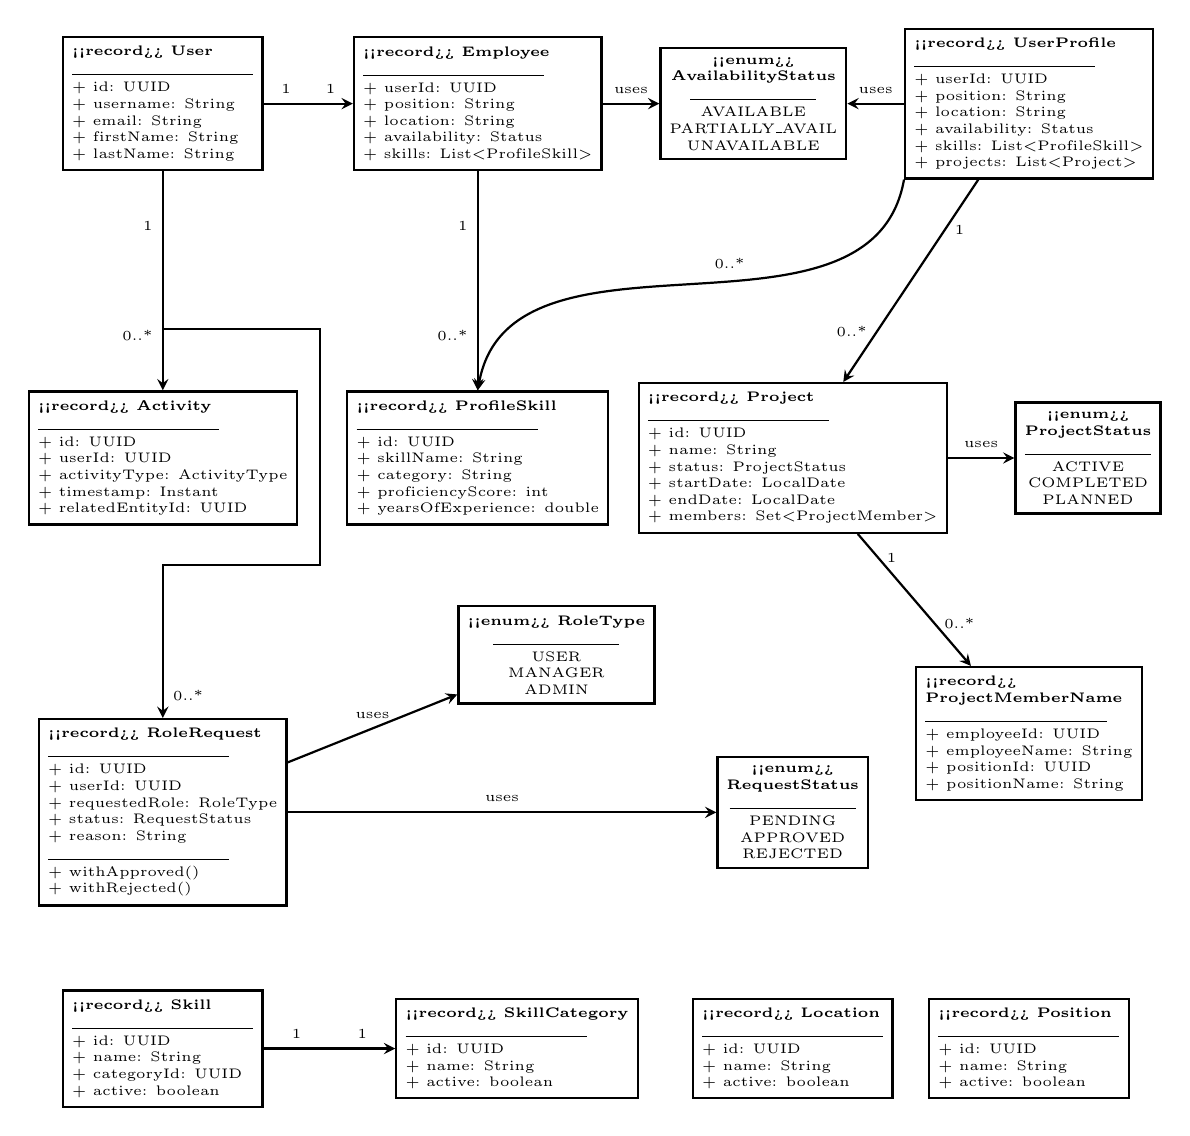
\begin{tikzpicture}[
    class/.style={rectangle, draw=black, thick, minimum width=2.5cm, minimum height=0.7cm, align=left, font=\tiny},
    enum/.style={rectangle, draw=black, thick, minimum width=1.8cm, minimum height=0.5cm, align=center, font=\tiny},
    arrow/.style={->,>=stealth,thick}
]

% ============== ROW 1: USER, EMPLOYEE, AVAILABILITYSTATUS, USERPROFILE ==============
\node[class] (user) at (0,0) {
    \textbf{<<record>> User}\\[1pt]
    \rule{2.3cm}{0.3pt}\\
    + id: UUID\\
    + username: String\\
    + email: String\\
    + firstName: String\\
    + lastName: String
};

\node[class] (employee) at (4,0) {
    \textbf{<<record>> Employee}\\[1pt]
    \rule{2.3cm}{0.3pt}\\
    + userId: UUID\\
    + position: String\\
    + location: String\\
    + availability: Status\\
    + skills: List<ProfileSkill>
};

\node[enum] (availStatus) at (7.5,0) {
    \textbf{<<enum>>}\\
    \textbf{AvailabilityStatus}\\[1pt]
    \rule{1.6cm}{0.3pt}\\
    AVAILABLE\\
    PARTIALLY\_AVAIL\\
    UNAVAILABLE
};

\node[class] (userProfile) at (11,0) {
    \textbf{<<record>> UserProfile}\\[1pt]
    \rule{2.3cm}{0.3pt}\\
    + userId: UUID\\
    + position: String\\
    + location: String\\
    + availability: Status\\
    + skills: List<ProfileSkill>\\
    + projects: List<Project>
};

% ============== ROW 2: ACTIVITY, PROFILESKILL, PROJECT, PROJECTSTATUS, PROJECTMEMBER ==============
\node[class] (activity) at (0,-4.5) {
    \textbf{<<record>> Activity}\\[1pt]
    \rule{2.3cm}{0.3pt}\\
    + id: UUID\\
    + userId: UUID\\
    + activityType: ActivityType\\
    + timestamp: Instant\\
    + relatedEntityId: UUID
};

\node[class] (profileSkill) at (4,-4.5) {
    \textbf{<<record>> ProfileSkill}\\[1pt]
    \rule{2.3cm}{0.3pt}\\
    + id: UUID\\
    + skillName: String\\
    + category: String\\
    + proficiencyScore: int\\
    + yearsOfExperience: double
};

\node[class] (project) at (8,-4.5) {
    \textbf{<<record>> Project}\\[1pt]
    \rule{2.3cm}{0.3pt}\\
    + id: UUID\\
    + name: String\\
    + status: ProjectStatus\\
    + startDate: LocalDate\\
    + endDate: LocalDate\\
    + members: Set<ProjectMember>
};

\node[enum] (projStatus) at (11.75,-4.5) {
    \textbf{<<enum>>}\\
    \textbf{ProjectStatus}\\[1pt]
    \rule{1.6cm}{0.3pt}\\
    ACTIVE\\
    COMPLETED\\
    PLANNED
};

\node[class] (projMember) at (11,-8) {
    \textbf{<<record>>}\\
    \textbf{ProjectMemberName}\\[1pt]
    \rule{2.3cm}{0.3pt}\\
    + employeeId: UUID\\
    + employeeName: String\\
    + positionId: UUID\\
    + positionName: String
};

% ============== ROW 3: ROLEREQUEST, ROLETYPE, REQUESTSTATUS ==============
\node[class] (roleReq) at (0,-9) {
    \textbf{<<record>> RoleRequest}\\[1pt]
    \rule{2.3cm}{0.3pt}\\
    + id: UUID\\
    + userId: UUID\\
    + requestedRole: RoleType\\
    + status: RequestStatus\\
    + reason: String\\[1pt]
    \rule{2.3cm}{0.3pt}\\
    + withApproved()\\
    + withRejected()
};

\node[enum] (roleType) at (5,-7) {
    \textbf{<<enum>> RoleType}\\[1pt]
    \rule{1.6cm}{0.3pt}\\
    USER\\
    MANAGER\\
    ADMIN
};

\node[enum] (reqStatus) at (8,-9) {
    \textbf{<<enum>>}\\
    \textbf{RequestStatus}\\[1pt]
    \rule{1.6cm}{0.3pt}\\
    PENDING\\
    APPROVED\\
    REJECTED
};

% ============== ROW 4: SKILL, SKILLCATEGORY, LOCATION, POSITION ==============
\node[class] (skill) at (0,-12) {
    \textbf{<<record>> Skill}\\[1pt]
    \rule{2.3cm}{0.3pt}\\
    + id: UUID\\
    + name: String\\
    + categoryId: UUID\\
    + active: boolean
};

\node[class] (skillCat) at (4.5,-12) {
    \textbf{<<record>> SkillCategory}\\[1pt]
    \rule{2.3cm}{0.3pt}\\
    + id: UUID\\
    + name: String\\
    + active: boolean
};

\node[class] (location) at (8,-12) {
    \textbf{<<record>> Location}\\[1pt]
    \rule{2.3cm}{0.3pt}\\
    + id: UUID\\
    + name: String\\
    + active: boolean
};

\node[class] (position) at (11,-12) {
    \textbf{<<record>> Position}\\[1pt]
    \rule{2.3cm}{0.3pt}\\
    + id: UUID\\
    + name: String\\
    + active: boolean
};

% ============== RELATIONSHIPS ==============

% User -> Employee
\draw[arrow] (user) -- (employee) node[near start,above,font=\tiny] {1} node[near end,above,font=\tiny] {1};

% Employee -> AvailabilityStatus
\draw[arrow] (employee) -- (availStatus) node[midway,above,font=\tiny] {uses};

% UserProfile -> AvailabilityStatus
\draw[arrow] (userProfile.west) -- (availStatus.east) node[midway,above,font=\tiny] {uses};

% User -> Activity (direkt vertikal!)
\draw[arrow] (user) -- (activity) node[near start,left,font=\tiny] {1} node[near end,left,font=\tiny] {0..*};

% Employee -> ProfileSkill
\draw[arrow] (employee) -- (profileSkill) node[near start,left,font=\tiny] {1} node[near end,left,font=\tiny] {0..*};

% UserProfile -> ProfileSkill
\draw[arrow,out=260,in=80] 
  (userProfile.south west) 
    to node[pos=0.4, left, font=\tiny, xshift=2pt, yshift=6pt] {0..*}
  (profileSkill.north);

% UserProfile -> Project
\draw[arrow] (userProfile) -- (project) node[near start,right,font=\tiny] {1} node[near end,left,font=\tiny] {0..*};

% Project -> ProjectStatus
\draw[arrow] (project) -- (projStatus) node[midway,above,font=\tiny] {uses};

% Project -> ProjectMember
\draw[arrow] 
  (project) -- (projMember)
    node[near start, above, font=\tiny, xshift=2pt, yshift=-2pt] {1}
    node[near end,   above, font=\tiny, xshift=6pt, yshift=-2pt] {0..*};

% Skill -> SkillCategory
\draw[arrow] (skill) -- (skillCat) node[near start,above,font=\tiny] {1} node[near end,above,font=\tiny] {1};

% User -> RoleRequest
\draw[arrow] 
    (user.south)
        -- ++(0,-2)
        -- ++(2,0)
        -- ++(0,-3)
        -- ++(-2,0)
        -- (roleReq.north)
        node[pos=0.85,right,font=\tiny] {0..*};

% RoleRequest -> RoleType
\draw[arrow] (roleReq) -- (roleType) node[midway,above,font=\tiny] {uses};

% RoleRequest -> RequestStatus
\draw[arrow] (roleReq.east) -- (reqStatus.west) node[midway,above,font=\tiny] {uses};

\end{tikzpicture}
\caption{Skill Management System: Domain Model - Kernentitäten}
\label{fig:domain_model_core}
\end{figure}

Das Klassendiagramm umfasst die gesamte Domain-Schicht mit zwölf Records 
(\textit{User, Employee, UserProfile, Activity, ProfileSkill, Project, 
ProjectMemberName, RoleRequest, Skill, SkillCategory, Location, Position}) 
sowie vier Enums (\textit{AvailabilityStatus, ProjectStatus, RoleType, RequestStatus}). 
Die wichtigsten Relationen sind u.\,a.\ \textbf{User 1:1 Employee}, 
\textbf{Employee 1:0..* ProfileSkill}, \textbf{Project 1:0..* ProjectMemberName} 
sowie weitere Verknüpfungen zwischen Skills, Kategorien, Position und Location.

Alle Domain-Objekte sind als immutable Java-Records implementiert; Enums werden über 
\textit{uses}-Beziehungen eingebunden und stellen typsichere Status- und Rollenwerte bereit. 
\textit{RoleRequest} ergänzt dies um Methoden für Statuswechsel 
(z.\,B.\ \texttt{withApproved()}, \texttt{withRejected()}).

Die Struktur folgt der Hexagonal Architecture und trennt Domain-Logik klar von 
Infrastrukturkomponenten (siehe Kapitel~3.3.1).

\subsection{Zustandsdiagramm}

\subsubsection{Rollenanfrage-Workflow}

Abbildung~\ref{fig:role_request_state} zeigt den Zustandsübergang für Self-Service Rollenanfragen:

\begin{figure}[H]
\centering
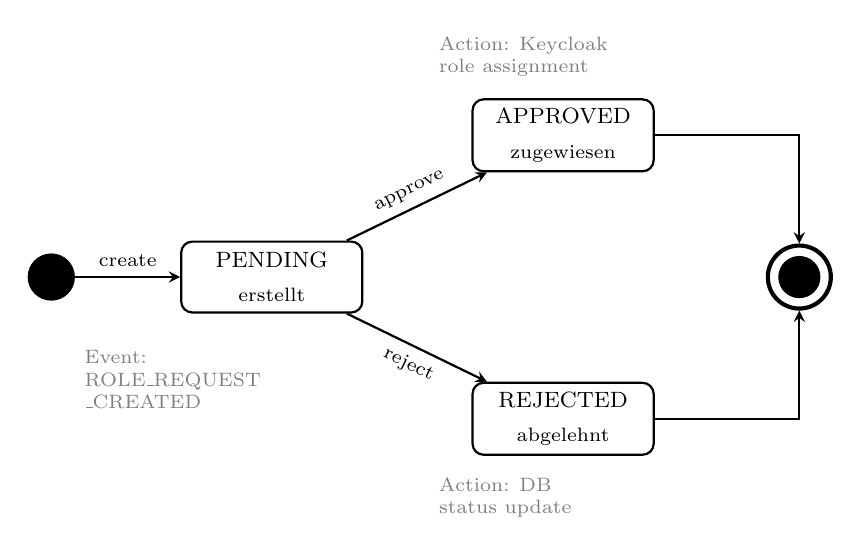
\begin{tikzpicture}[
    state/.style={rectangle, rounded corners, draw=black, thick, minimum width=2.3cm, minimum height=0.9cm, align=center, font=\footnotesize},
    initial/.style={circle, fill=black, minimum size=0.6cm},
    final/.style={circle, draw=black, line width=1.5pt, minimum size=0.8cm,
                  path picture={\draw[line width=1pt, fill=black] 
                  (path picture bounding box.center) circle (0.25cm);}},
    arrow/.style={->,>=stealth,thick}
]

% States
\node[initial] (init) at (0,0) {};
\node[state] (pending) at (2.8,0) {PENDING\\[3pt]{\scriptsize erstellt}};
\node[state] (approved) at (6.5,1.8) {APPROVED\\[3pt]{\scriptsize zugewiesen}};
\node[state] (rejected) at (6.5,-1.8) {REJECTED\\[3pt]{\scriptsize abgelehnt}};
\node[final] (end) at (9.5,0) {};

% Transitions
\draw[arrow] (init) -- (pending) node[midway,above,font=\scriptsize] {create};
\draw[arrow] (pending) -- (approved) node[midway,above,sloped,font=\scriptsize] {approve};
\draw[arrow] (pending) -- (rejected) node[midway,below,sloped,font=\scriptsize] {reject};
\draw[arrow] (approved) -| (end);
\draw[arrow] (rejected) -| (end);

% Events/Actions - outside flow
\node[font=\scriptsize, text=gray, align=left, anchor=west] at (0.3,-1.3) {
    Event:\\
    ROLE\_REQUEST\\
    \_CREATED
};
\node[font=\scriptsize, text=gray, align=left, anchor=west] at (4.8,2.8) {
    Action: Keycloak\\
    role assignment
};
\node[font=\scriptsize, text=gray, align=left, anchor=west] at (4.8,-2.8) {
    Action: DB\\
    status update
};

\end{tikzpicture}
\caption{Zustandsdiagramm: Rollenanfrage-Workflow (Self-Service Pattern)}
\label{fig:role_request_state}
\end{figure}

Der Rollenanfrage-Workflow ermöglicht Self-Service-Rollenverwaltung:
\begin{enumerate}[noitemsep]
    \item \textbf{PENDING}: User erstellt Anfrage für MANAGER-Rolle (V14 Migration)
    \item \textbf{APPROVED}: Admin genehmigt → Backend weist Rolle in Keycloak zu → Status-Update in DB → Activity-Log-Eintrag
    \item \textbf{REJECTED}: Admin lehnt ab → Status-Update in DB → Activity-Log-Eintrag
\end{enumerate}

Das Zustandsdiagramm dokumentiert den Self-Service-Ansatz für Rechteverwaltung (siehe Kapitel 3.4.3).

% ==========================================
% A.3 QUALITÄTSSICHERUNG & CI/CD
% ==========================================

\section{Qualitätssicherung \& CI/CD}

\subsection{Code-Qualitätsmetriken}

\begin{table}[H]
\centering
\footnotesize
\rowcolors{2}{EDAGDunkelgrau!10}{white}
\begin{tabularx}{\textwidth}{|p{3.5cm}|p{2.5cm}|p{2.5cm}|X|}
\hline
\rowcolor{EDAGDunkelgrau!10}
\textbf{Metrik} & \textbf{Backend} & \textbf{Frontend} & \textbf{Bewertung} \\
\hline
Lines of Code & 7.800+ & 10.500+ & Vollständige Implementierung \\
\hline
Maintainability Rating & A & A & Hohe Wartbarkeit, klar strukturiert \\
\hline
Security Rating & A & A & Keine Security Hotspots \\
\hline
Reliability Rating & A & A & Keine kritischen Bugs \\
\hline
Test Coverage & 0\% & 0\% & Keine automatisierten Tests \\
\hline
Duplications & < 1\% & < 2\% & Minimale Code-Redundanz \\
\hline
\end{tabularx}
\caption{SonarQube Code-Qualitätsmetriken (Stand: Build \#15)}
\label{tab:sonarqube_metrics_detail}
\end{table}

\subsection{CI/CD und Quality Assurance}

\subsubsection{Commit-Historie und Conventional Commits}

\begin{figure}[H]
\centering
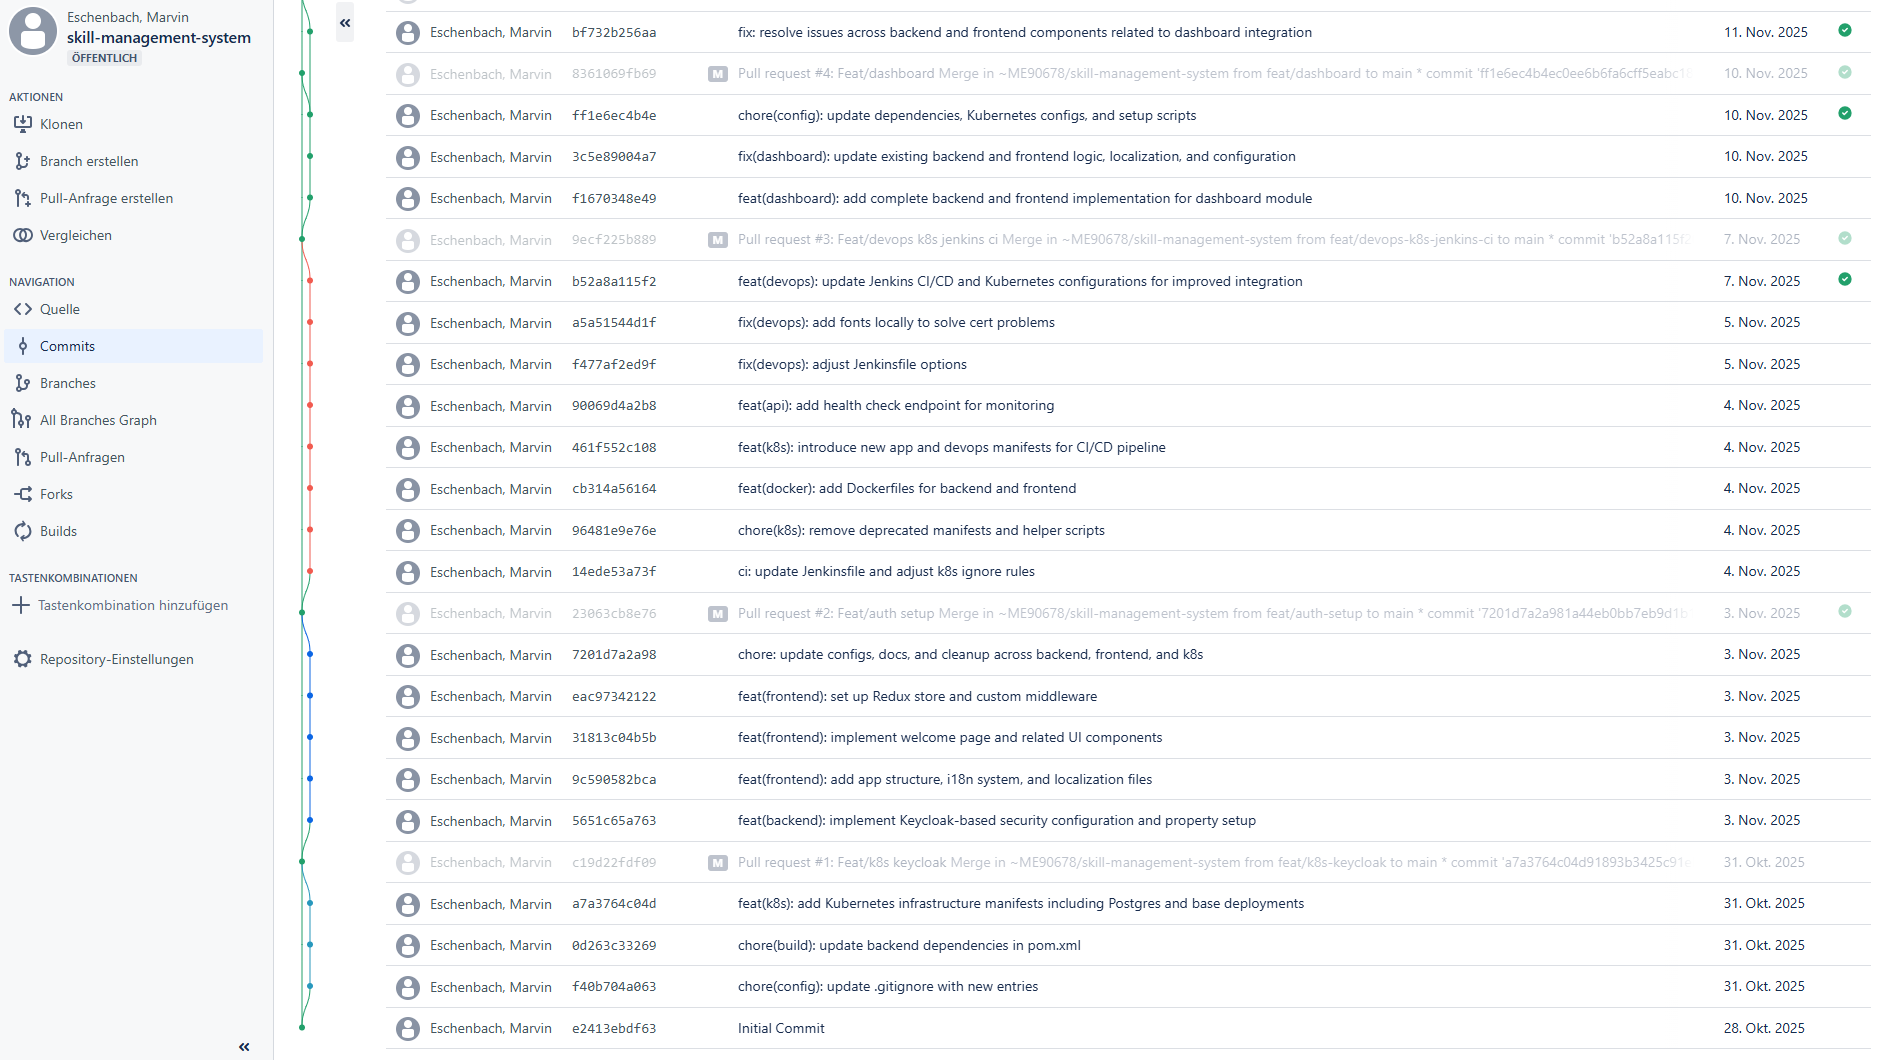
\includegraphics[width=0.95\textwidth]{references/commits.png}
\caption{Commit-Historie mit Conventional Commits und Commit Lint}
\label{fig:commits}
\end{figure}

Abbildung~\ref{fig:commits} zeigt die strukturierte Commit-Historie nach Conventional Commits-Standard mit Commit Lint-Validierung. Die Commit-Messages folgen dem Format \texttt{type(scope): description} und ermöglichen automatisches Changelog-Generation und semantische Versionierung.

\subsubsection{SonarQube Code-Analyse}

\paragraph{Backend Quality Gate}

\begin{figure}[H]
\centering
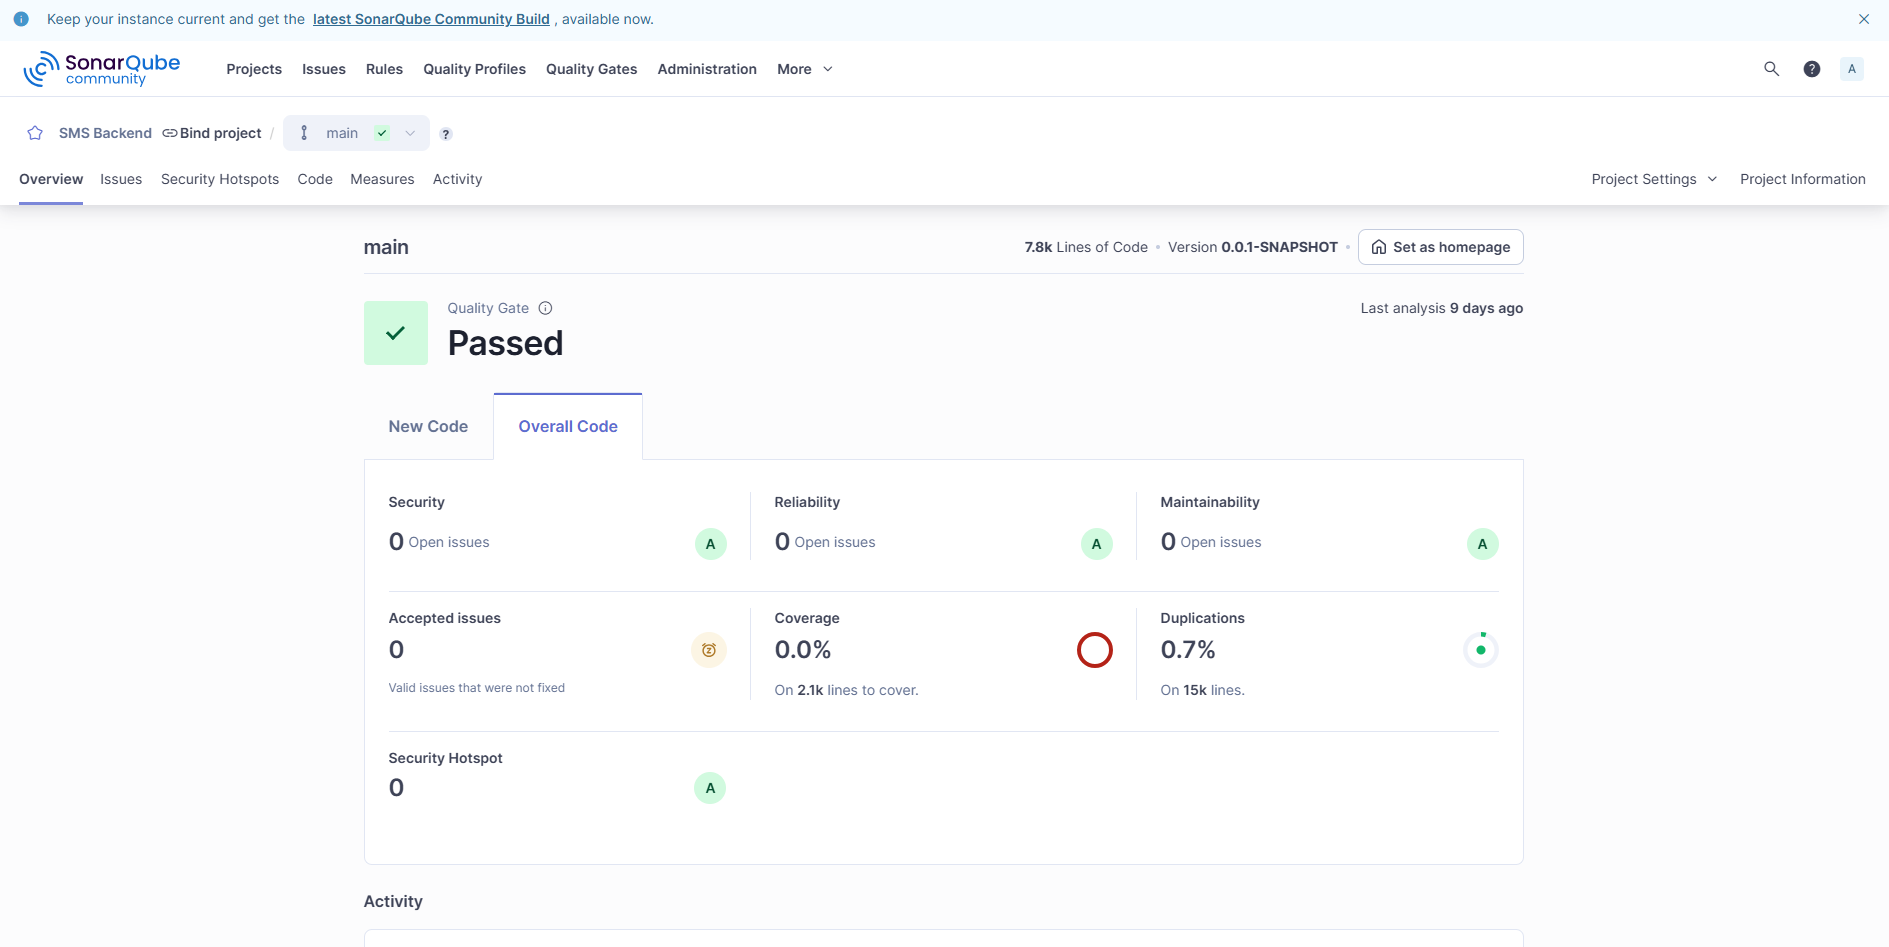
\includegraphics[width=0.95\textwidth]{references/sonar-backend.png}
\caption{SonarQube Analyse -- Backend (SMS Backend, Branch: main)}
\label{fig:sonarqube_backend}
\end{figure}

Abbildung~\ref{fig:sonarqube_backend} zeigt die SonarQube-Analyse des Backend-Projekts mit Quality Gate \textit{Passed}. Die Metriken umfassen 7.800+ Lines of Code, 0 Open Issues in allen Kategorien (Security, Reliability, Maintainability jeweils Rating A), 0.7\% Duplications und 15k Lines to Cover (bei 0\% Test Coverage).

\paragraph{Frontend Quality Gate}

\begin{figure}[H]
\centering
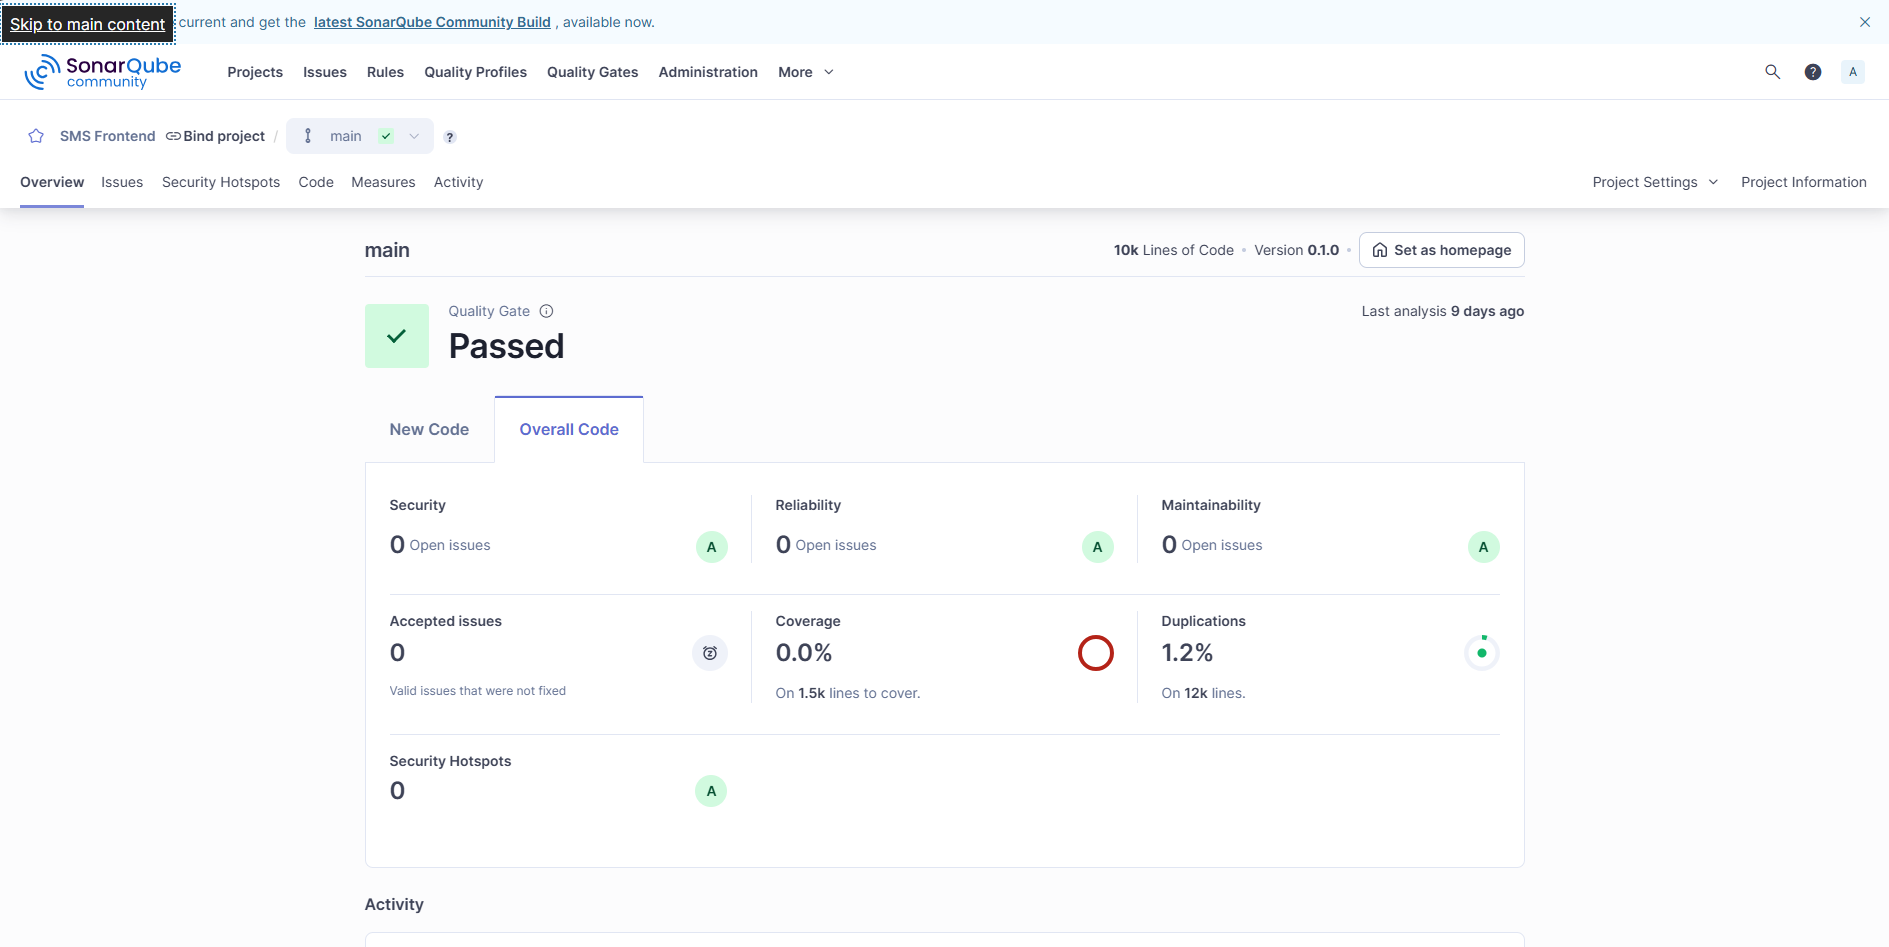
\includegraphics[width=0.95\textwidth]{references/sonar-frontend.png}
\caption{SonarQube Analyse -- Frontend (SMS Frontend, Branch: main)}
\label{fig:sonarqube_frontend}
\end{figure}

Abbildung~\ref{fig:sonarqube_frontend} zeigt die SonarQube-Analyse des Frontend-Projekts mit Quality Gate \textit{Passed}. Die Metriken umfassen 10.500+ Lines of Code, 0 Open Issues (Security/Reliability/Maintainability jeweils Rating A), 1.2\% Duplications und 12k Lines to Cover.

\subsubsection{Jenkins CI/CD Pipeline}

\begin{figure}[H]
\centering
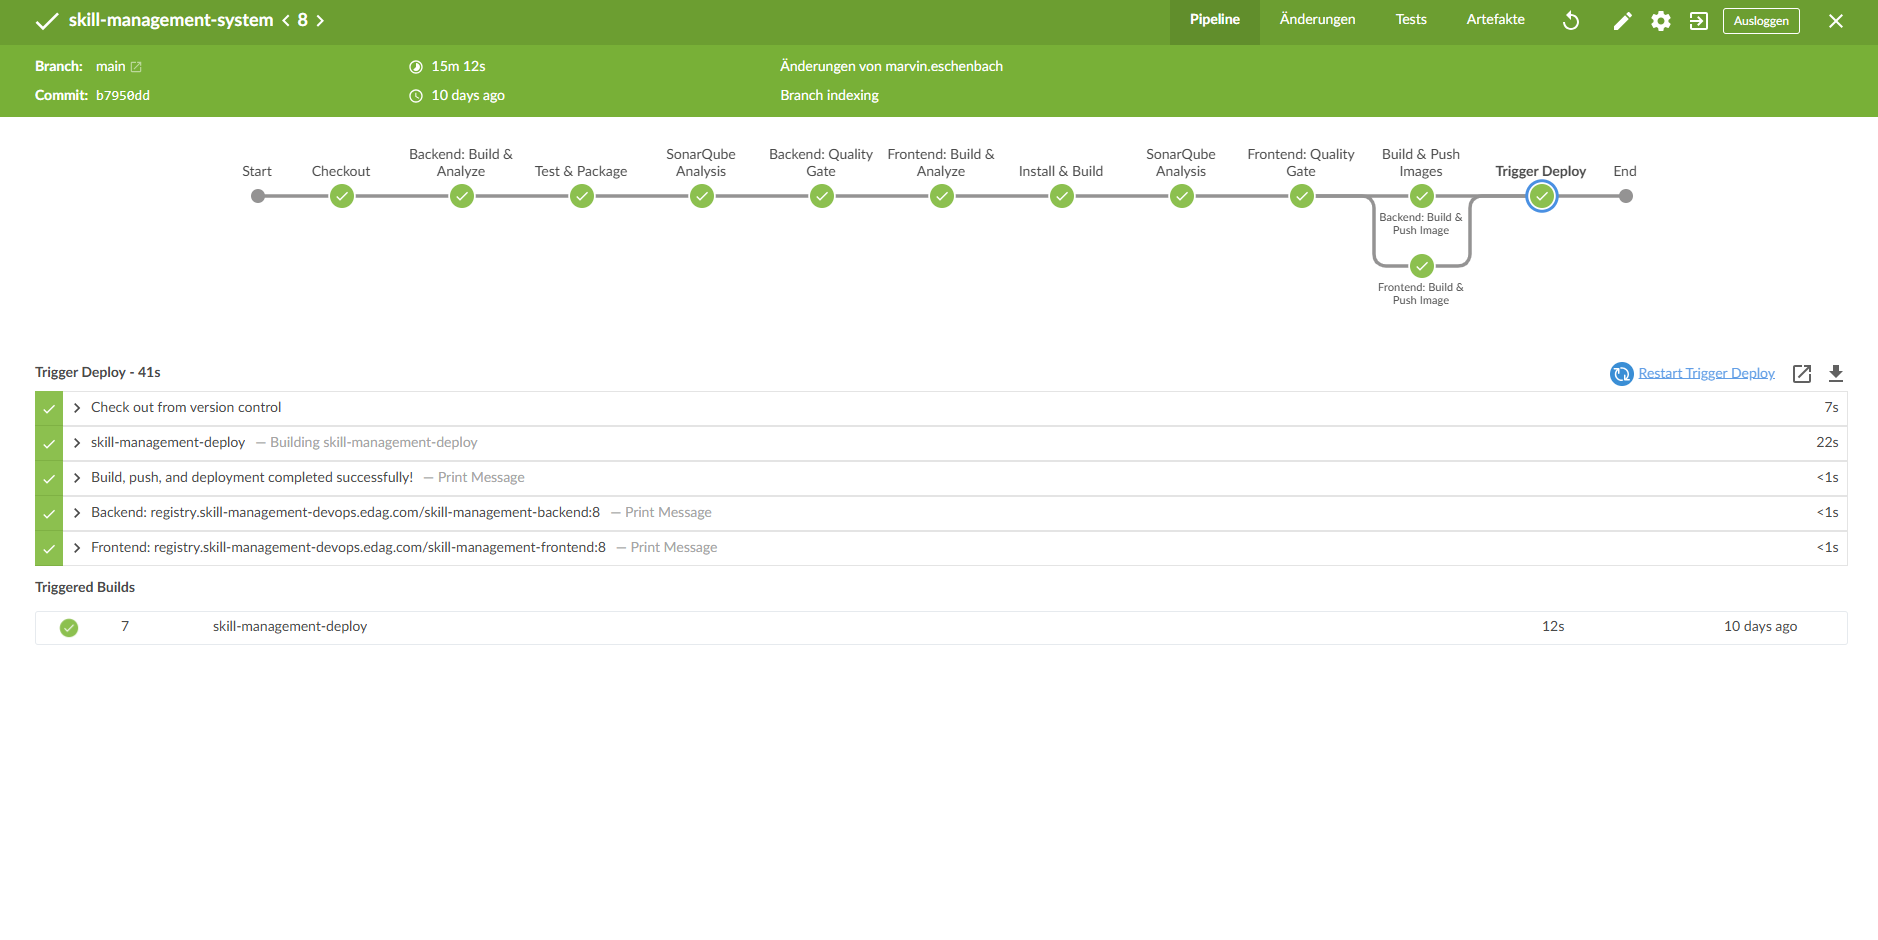
\includegraphics[width=0.95\textwidth]{references/pipeline.png}
\caption{Jenkins Declarative Pipeline -- Build \#7 (Trigger Deploy Stage)}
\label{fig:jenkins_pipeline}
\end{figure}

Abbildung~\ref{fig:jenkins_pipeline} zeigt die vollständige Jenkins Pipeline-Ausführung mit allen Stages: Checkout (7s), Backend Build \& Analyze (22s), Frontend Build \& Analyze (Build \& Push Images parallel: Backend 12s, Frontend <1s), Trigger Deploy (41s). Die Gesamtlaufzeit betrug 15 Minuten 12 Sekunden. Die Pipeline-Visualisierung zeigt den erfolgreichen Deployment-Prozess vom Branch \texttt{main} mit automatischer Image-Erstellung und Kubernetes-Deployment.

\subsubsection{Jenkinsfile Deklaration}

\begin{lstlisting}[language=bash, caption=Jenkins Declarative Pipeline -- Jenkinsfile, label=lst:jenkinsfile]
pipeline {
  agent none
  options {
    disableConcurrentBuilds()
    timeout(time: 1, unit: 'HOURS')
  }
  environment {
    REGISTRY_EXTERNAL = 'registry.skill-management-devops.edag.com'
    BACKEND_IMAGE_EXTERNAL = "\${REGISTRY_EXTERNAL}/skill-management-backend"
    FRONTEND_IMAGE_EXTERNAL = "\${REGISTRY_EXTERNAL}/skill-management-frontend"
  }
  stages {
    stage('Checkout') {
      agent { label 'universal' }
      steps { checkout scm }
    }
    stage('Backend: Build & Analyze') {
      agent { label 'backend' }
      stages {
        stage('Test & Package') {
          steps {
            container('maven') {
              sh '''#!/bin/bash
                cd backend
                ./mvnw -B clean test package
              '''
            }
          }
        }
        stage('SonarQube Analysis') {
          steps {
            container('maven') {
              withSonarQubeEnv('SonarQube') {
                sh '''cd backend
                  ./mvnw sonar:sonar \\
                    -Dsonar.projectKey=sms-backend
                '''
              }
            }
          }
        }
      }
    }
    stage('Backend: Quality Gate') {
      agent { label 'universal' }
      steps {
        timeout(time: 10, unit: 'MINUTES') {
          waitForQualityGate abortPipeline: true
        }
      }
    }
    // Frontend stages analog zu Backend
    stage('Build & Push Images') {
      when { branch 'main' }
      parallel {
        stage('Backend: Build & Push Image') {
          agent { label 'backend' }
          steps {
            container('docker') {
              script {
                docker.withRegistry(
                  "https://\${REGISTRY_EXTERNAL}", 'docker-registry') {
                  dir('backend') {
                    def img = docker.build(
                      "\${BACKEND_IMAGE_EXTERNAL}:\${BUILD_NUMBER}")
                    img.push()
                    img.push('latest')
                  }
                }
              }
            }
          }
        }
        // Frontend parallel
      }
    }
    stage('Trigger Deploy') {
      when { branch 'main' }
      agent { label 'universal' }
      steps {
        script { build job: 'skill-management-deploy' }
      }
    }
  }
}
\end{lstlisting}

Die Jenkinsfile-Konfiguration (Listing~\ref{lst:jenkinsfile}) definiert eine mehrstufige Pipeline mit Kubernetes-Agents für unterschiedliche Build-Environments (Backend: Maven, Frontend: Node.js, Docker: Image-Builds). Quality Gates stoppen die Pipeline bei SonarQube-Violations. Branch \texttt{main} triggert automatisch Docker-Image-Builds und Deployment.

\subsubsection{Lighthouse Performance Audit}

\begin{figure}[H]
\centering
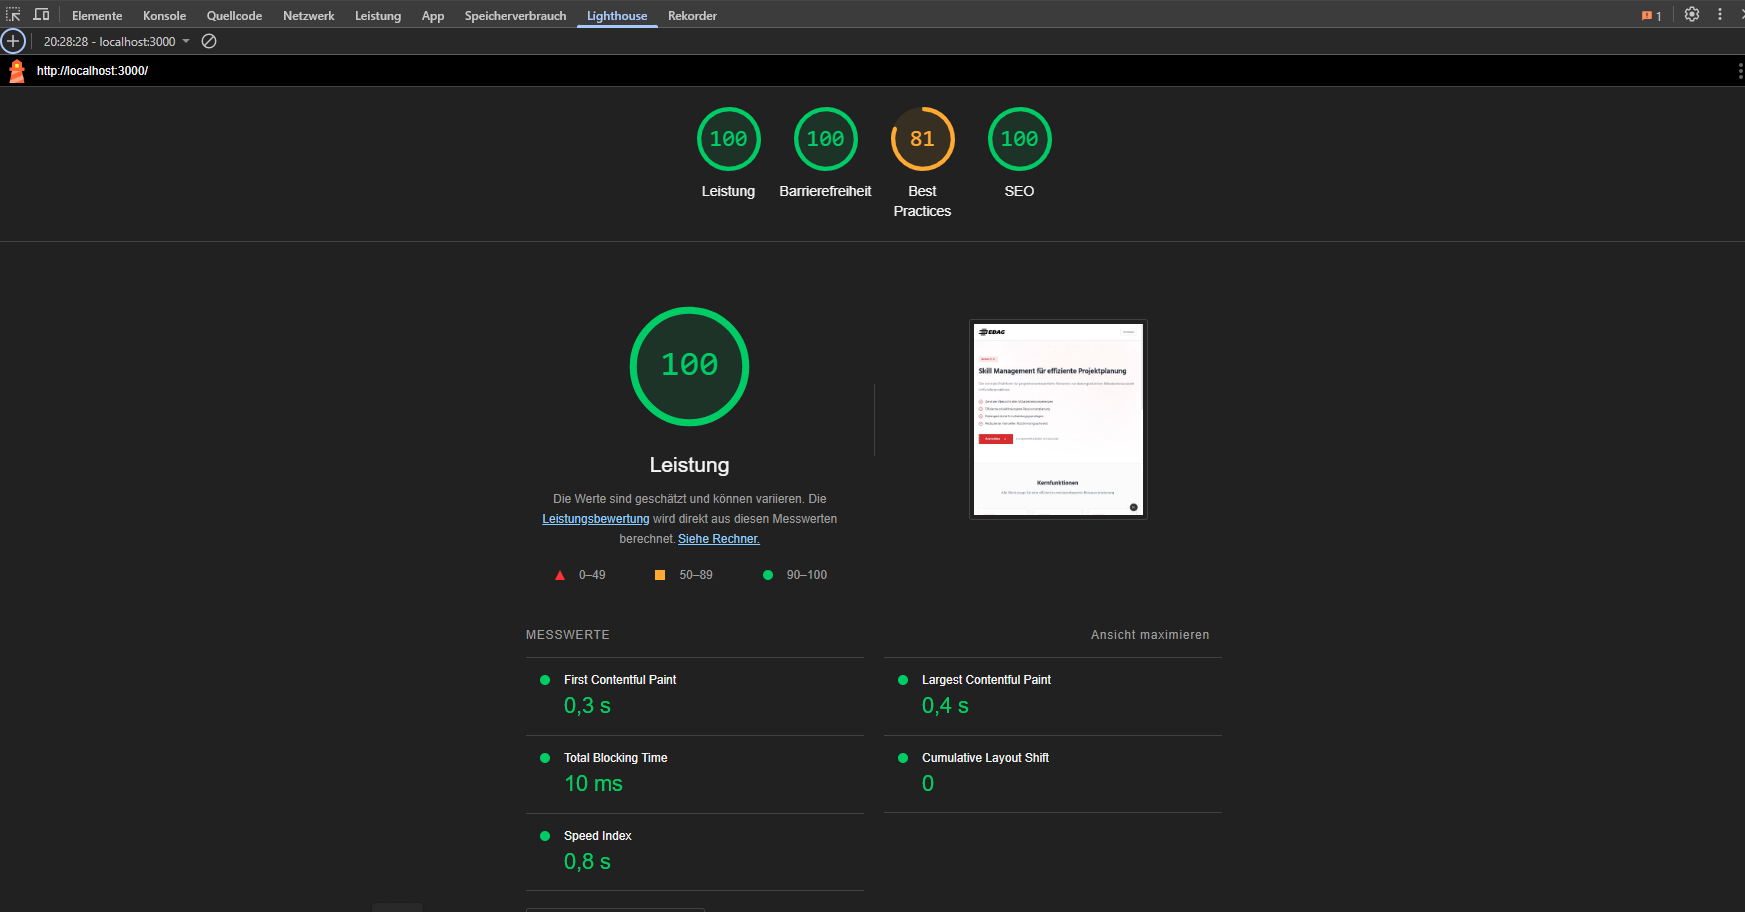
\includegraphics[width=0.90\textwidth]{references/lighthouse-welcome.png}
\caption{Google Lighthouse Audit -- Welcome Screen (Performance: 100, Best Practices: 81)}
\label{fig:lighthouse_welcome}
\end{figure}

Abbildung~\ref{fig:lighthouse_welcome} zeigt das Lighthouse-Audit\cite{lighthouse_docs} der Welcome-Seite mit exzellenten Werten: Performance 100/100 (First Contentful Paint 0.3s, Largest Contentful Paint 0.4s, Speed Index 0.8s), Accessibility 100/100, Best Practices 81/100, SEO 100/100. Die Messwerte bestätigen die Performance-Anforderungen aus Kapitel~\ref{sec:nicht_funktionale_anforderungen}.

% ==========================================
% A.4 DEPLOYMENT & KONFIGURATION
% ==========================================

\section{Deployment \& Konfiguration}

\subsection{ER-Datenmodell}
\label{sec:er_model}

\begin{figure}[H]
\centering
\begin{tikzpicture}[
    scale=1.0,
    every node/.style={transform shape},
    entity/.style={rectangle, draw, minimum width=2.5cm, minimum height=0.8cm, font=\small, align=center},
    attribute/.style={ellipse, draw, minimum width=1.5cm, minimum height=0.6cm, font=\tiny, align=center},
    key/.style={ellipse, draw, minimum width=1.5cm, minimum height=0.6cm, font=\tiny, align=center, font=\tiny\bfseries},
    relation/.style={diamond, draw, minimum width=1.8cm, minimum height=1cm, font=\scriptsize, align=center, aspect=2},
    line/.style={-}
]

% Entitäten - Optimierte Positionierung
\node[entity] (user) at (0,8) {\textbf{users}};
\node[entity] (profile) at (6,8) {\textbf{employee\_profiles}};
\node[entity] (skill) at (10,8) {\textbf{skills}};
\node[entity] (category) at (10,2) {\textbf{skill\_categories}};
\node[entity] (project) at (3,5) {\textbf{projects}};
\node[entity] (stats) at (0,3.5) {\textbf{user\_statistics}};

% Beziehungen (Rauten)
\node[relation] (r1) at (3,8) {has};
\node[relation] (r2) at (8.5,6.5) {possesses};
\node[relation] (r3) at (12,4) {belongs\\to};
\node[relation] (r4) at (1.5,6.5) {owns};
\node[relation] (r5) at (6,4) {contains};
\node[relation] (r6) at (0,5.5) {tracks};

% Primärschlüssel (PK)
\node[key] (user_id) at (-1,7.1) {\underline{id}};
\node[key] (profile_id) at (5,7) {\underline{user\_id}};
\node[key] (skill_id) at (12.2,8) {\underline{id}};
\node[key] (cat_id) at (12.5,2) {\underline{id}};
\node[key] (proj_id) at (2.5,4) {\underline{id}};
\node[key] (stats_id) at (0,2.5) {\underline{user\_id}};

% Fremdschlüssel (FK)
\node[attribute] (skill_cat_fk) at (12,7) {category\_id};
\node[attribute] (proj_created_fk) at (3.5,6) {created\_by\\\_user\_id};

% Attribute employee_skills (m:n)
\node[key] (es_emp) at (7.5,4.9) {\underline{employee\_id}};
\node[key] (es_skill) at (10.5,4.9) {\underline{skill\_id}};
\node[attribute] (es_id) at (9,5.5) {id};

% Attribute project_members (m:n)
\node[key] (pm_proj) at (4.5,3) {\underline{project\_id}};
\node[key] (pm_emp) at (8,3) {\underline{employee\_id}};
\node[attribute] (pm_id) at (6,2.2) {id};

% Verbindungen Entitäten zu Attributen
\draw[line] (user) -- (user_id);
\draw[line] (profile) -- (profile_id);
\draw[line] (skill) -- (skill_id);
\draw[line] (skill) -- (skill_cat_fk);
\draw[line] (category) -- (cat_id);
\draw[line] (project) -- (proj_id);
\draw[line] (project) -- (proj_created_fk);
\draw[line] (stats) -- (stats_id);

% Verbindungen m:n-Beziehungen zu Attributen
\draw[line] (r2) -- (es_emp);
\draw[line] (r2) -- (es_skill);
\draw[line] (r2) -- (es_id);
\draw[line] (r5) -- (pm_proj);
\draw[line] (r5) -- (pm_emp);
\draw[line] (r5) -- (pm_id);

% Beziehungen mit Kardinalitäten
\draw[line] (user) -- node[above, font=\small] {1} (r1);
\draw[line] (r1) -- node[above, font=\small] {1} (profile);

\draw[line] (profile) -- node[above left, font=\small] {n} (r2);
\draw[line] (r2) -- node[above right, font=\small] {m} (skill);

\draw[line] (skill) -- node[right, font=\small] {n} (r3);
\draw[line] (r3) -- node[right, font=\small] {1} (category);

\draw[line] (user) -- node[left, font=\small] {1} (r4);
\draw[line] (r4) -- node[left, font=\small] {n} (project);

\draw[line] (project) -- node[above, font=\small] {n} (r5);
\draw[line] (r5) -- node[below right, font=\small] {m} (profile);

\draw[line] (user) -- node[left, font=\small] {1} (r6);
\draw[line] (r6) -- node[left, font=\small] {1} (stats);

\end{tikzpicture}
\caption{Entity-Relationship-Diagramm nach UML-Standard (Kernentitäten)}
\label{fig:erd}
\end{figure}

\subsubsection{Datenbankmodell}

Abbildung~\ref{fig:db_screenshot} zeigt die tatsächliche Datenbankstruktur mit allen 15 Tabellen (14 Anwendungstabellen + \texttt{flyway\_schema\_history}), ihren Spalten, Datentypen und Constraints.

\begin{figure}[H]
\centering
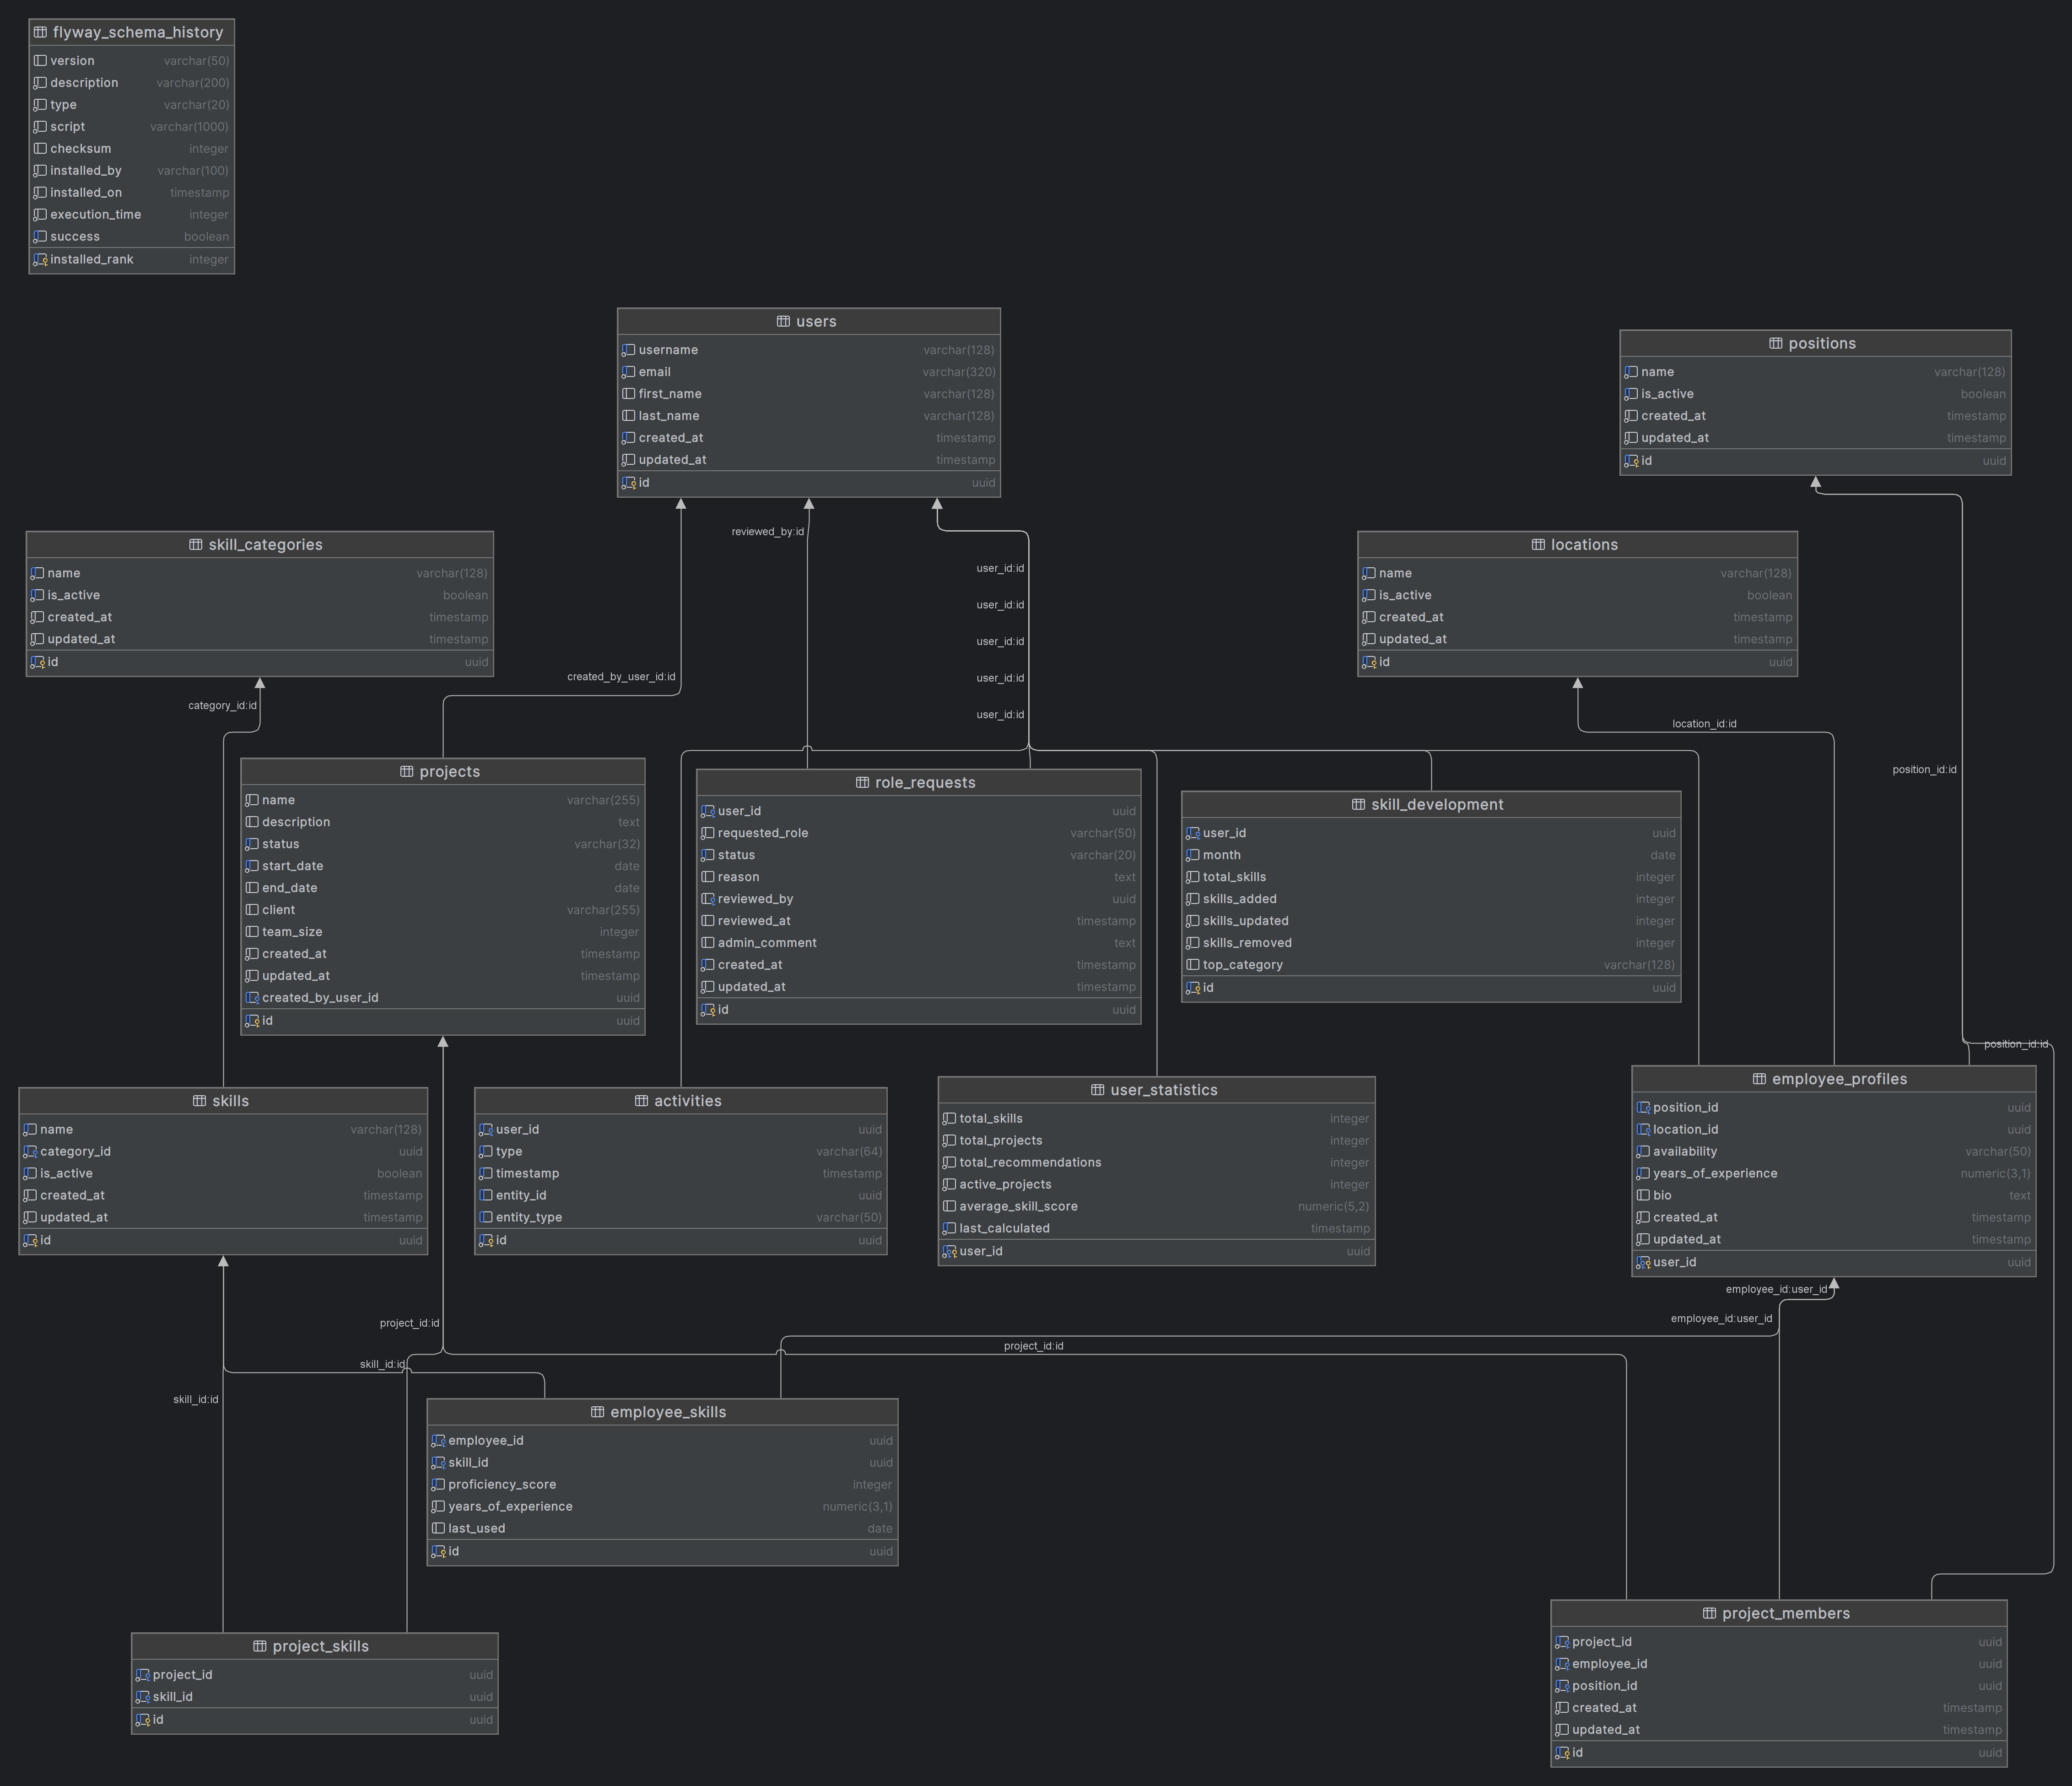
\includegraphics[width=0.95\textwidth]{references/skillmanagement@localhost.png}
\caption{Datenbank-Schema: Vollständige Tabellenstruktur mit 15 Tabellen}
\label{fig:db_screenshot}
\end{figure}

\subsection{Datenbank-Migrationen}
\label{sec:db_migrations}

Die 15 Flyway-Migrationsskripte dokumentieren die vollständige Datenbank-Evolution von Basis-Tabellen über automatisierte Trigger bis zu umfassenden Analytics. Die versionierte Schema-Migration gewährleistet reproduzierbare Deployments und nachvollziehbare Änderungen.

\subsubsection{Migrations-Übersicht}

\begin{table}[H]
\centering
\footnotesize
\rowcolors{2}{EDAGDunkelgrau!10}{white}
\begin{tabularx}{\textwidth}{|l|l|X|r|}
\hline
\rowcolor{EDAGDunkelgrau!10}
\textbf{Nr.} & \textbf{Kategorie} & \textbf{Beschreibung} & \textbf{LOC} \\
\hline
V1 & Schema & users, positions, locations, skill\_categories, skills & 92 \\
\hline
V2 & Schema & employee\_profiles, employee\_skills (Junction) & 56 \\
\hline
V3 & Schema & projects, project\_skills, project\_positions & 143 \\
\hline
V4 & Analytics & user\_statistics, skill\_development, activities & 102 \\
\hline
V5 & Trigger & Automatische updated\_at-Timestamps (7 Tabellen) & 48 \\
\hline
V6 & Trigger & Echtzeit-Aggregation: total\_skills, avg\_score, project\_counts & 131 \\
\hline
V7 & Trigger & Audit-Trail: SKILL\_ADDED, PROJECT\_CREATED, PROFILE\_UPDATED & 134 \\
\hline
V8 & Trigger & Monatliche Skill-Entwicklung Snapshots & 177 \\
\hline
V9 & Daten & 200+ Skills, 55+ Positionen, 30 Standorte & 379 \\
\hline
V10 & Trigger & Auto-Erstellung employee\_profiles bei User-Insert & 47 \\
\hline
V11 & Refactoring & project\_members n:m-Tabelle (eliminiert Redundanz) & 278 \\
\hline
V12 & Trigger & Automatische Team-Size-Berechnung & 36 \\
\hline
V13 & Refactoring & Entfernung team\_size CHECK-Constraint & 7 \\
\hline
V14 & Schema & role\_requests (Self-Service Rollenanfragen) & 38 \\
\hline
V15 & Trigger & 30+ Event-Typen: ROLE\_REQUEST\_APPROVED, PROJECT\_MEMBER\_ADDED & 358 \\
\hline
\rowcolor{EDAGDunkelgrau!30}
\textbf{Gesamt} & \textbf{15 Dateien} & \textbf{Vollständig versioniertes Datenbankschema} & \textbf{2.026} \\
\hline
\end{tabularx}
\caption{Vollständige Übersicht aller Flyway-Datenbank-Migrationen}
\label{tab:db_migrations}
\end{table}

\paragraph{Beispiel-Listings}

Die folgenden Auszüge zeigen exemplarisch die Struktur der ersten zwei Migrationen. Alle weiteren 13 Migrationen folgen dem gleichen Schema mit vollständiger Dokumentation durch SQL-Kommentare.

\subparagraph{V1: Basis-Tabellen (Auszug)}\mbox{}\vspace{4pt}

\begin{lstlisting}[language=SQL, basicstyle=\scriptsize\ttfamily, frame=single]
-- V1__create_base_tables.sql
CREATE EXTENSION IF NOT EXISTS pg_trgm; -- Full-text search

CREATE TABLE users (
    id UUID PRIMARY KEY DEFAULT gen_random_uuid(),
    username VARCHAR(128) NOT NULL UNIQUE,
    email VARCHAR(320) NOT NULL UNIQUE,
    first_name VARCHAR(128),
    last_name VARCHAR(128),
    created_at TIMESTAMP NOT NULL DEFAULT CURRENT_TIMESTAMP
);

CREATE TABLE skills (
    id UUID PRIMARY KEY DEFAULT gen_random_uuid(),
    name VARCHAR(128) NOT NULL UNIQUE,
    category_id UUID NOT NULL,
    CONSTRAINT fk_skills_category FOREIGN KEY (category_id)
        REFERENCES skill_categories(id) ON DELETE RESTRICT
);
\end{lstlisting}

\subparagraph{V2: Employee Skills Junction-Tabelle (Auszug)}\mbox{}\vspace{4pt}

\begin{lstlisting}[language=SQL, basicstyle=\scriptsize\ttfamily, frame=single]
-- V2__create_employee_profiles.sql
CREATE TABLE employee_skills (
    id UUID PRIMARY KEY DEFAULT gen_random_uuid(),
    employee_id UUID NOT NULL,
    skill_id UUID NOT NULL,
    proficiency_score INTEGER NOT NULL,
    CONSTRAINT fk_employee_skill_employee FOREIGN KEY (employee_id)
        REFERENCES employee_profiles(user_id) ON DELETE CASCADE,
    CONSTRAINT chk_proficiency_score CHECK 
        (proficiency_score >= 0 AND proficiency_score <= 100)
);
\end{lstlisting}

\vspace{1em}

\noindent\textbf{Repository-Pfad:} Alle 15 vollständigen SQL-Migrationsskripte (2.026 LOC) sind verfügbar unter:\\ 
\texttt{backend/src/main/resources/db/migration/V*.sql}

\subsection{Kubernetes Ingress-Konfiguration}

\begin{table}[H]
\centering
\footnotesize
\rowcolors{2}{EDAGDunkelgrau!10}{white}
\begin{tabularx}{\textwidth}{|p{4.5cm}|p{3cm}|X|}
\hline
\rowcolor{EDAGDunkelgrau!10}
\textbf{Hostname} & \textbf{Service} & \textbf{Beschreibung} \\
\hline
keycloak.dev.local & keycloak:8080 & Identity Provider (Dev) \\
\hline
skill-management.edag.com & frontend:3000 & Next.js Frontend (Prod) \\
\hline
api.skill-management.edag.com & backend:8080 & Spring Boot Backend (Prod) \\
\hline
keycloak.skill-management.edag.com & keycloak:8080 & Keycloak IAM (Prod) \\
\hline
jenkins.devops.local & jenkins:8080 & CI/CD Pipeline \\
\hline
sonarqube.devops.local & sonarqube:9000 & Code-Qualität \\
\hline
registry.devops.local & docker-registry:5000 & Docker Registry \\
\hline
\end{tabularx}
\caption{Traefik Ingress-Konfiguration für alle Environments}
\label{tab:ingress_config}
\end{table}

% ==========================================
% A.5 DOKUMENTATION
% ==========================================

\section{Dokumentation}

\subsection{UI-Screenshots}
\label{sec:ui_screenshots}

\subsubsection{Authentifizierung und Onboarding}

\begin{figure}[H]
\centering
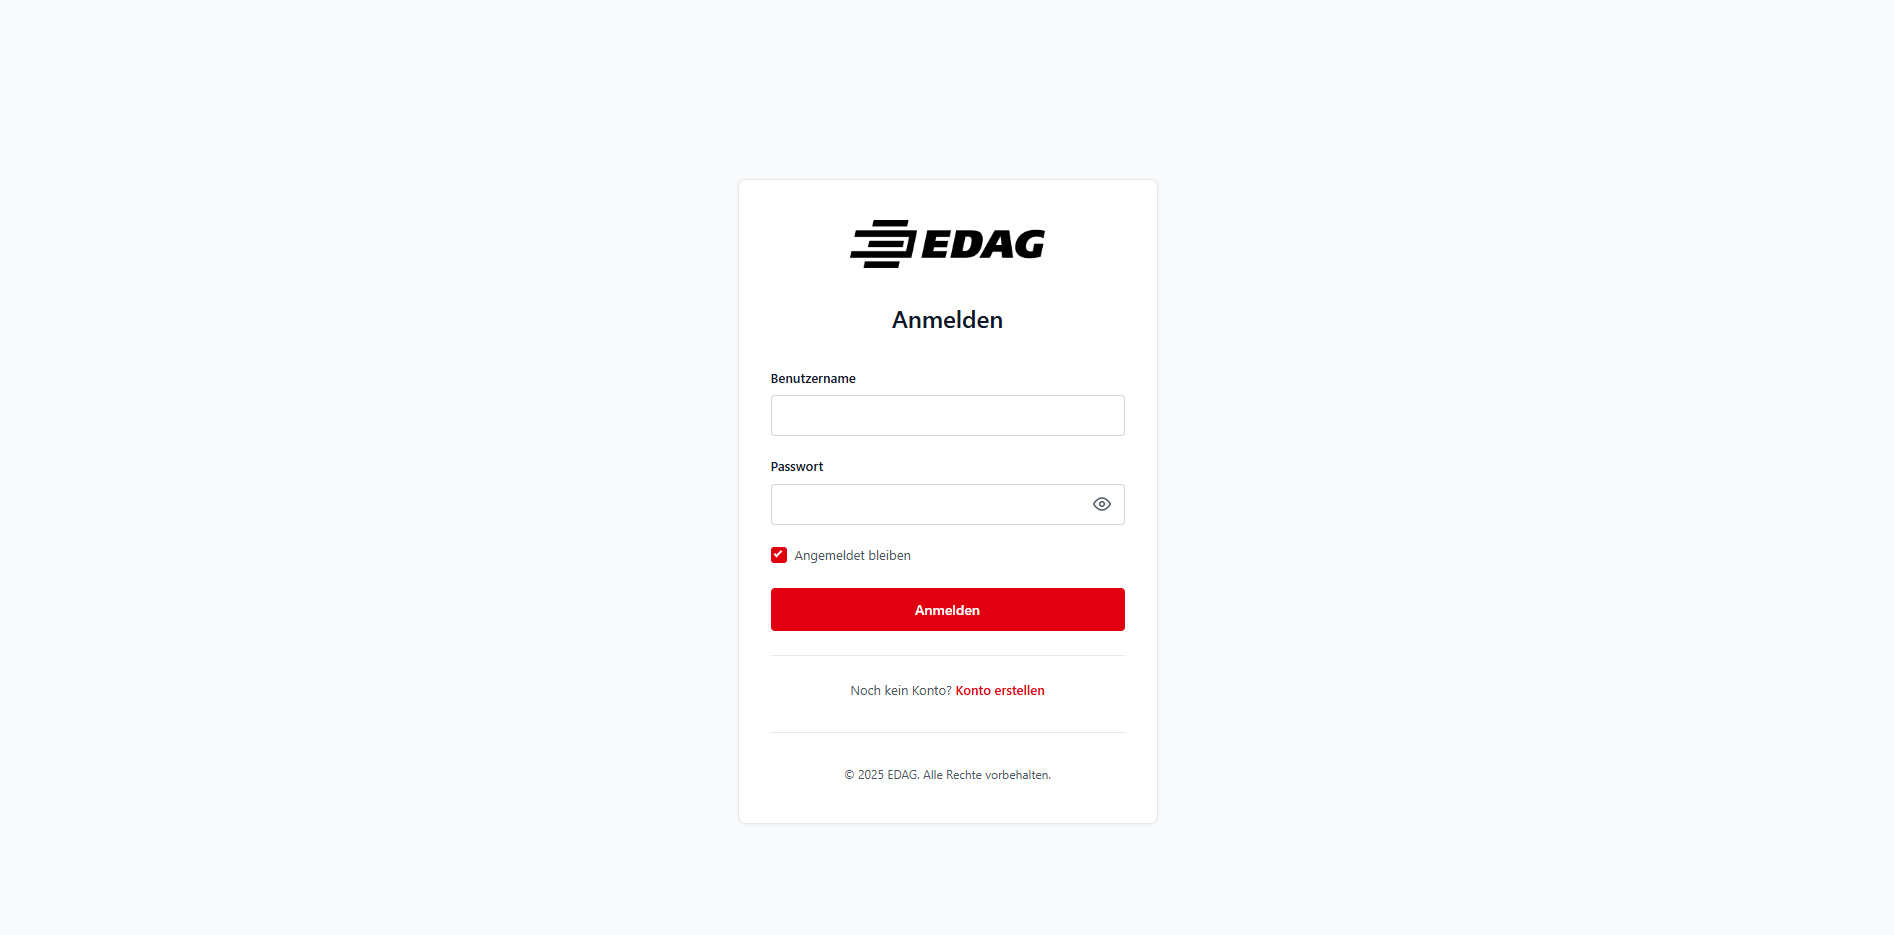
\includegraphics[width=0.9\textwidth]{references/ui-login-1.png}
\caption{Login-Seite mit Keycloak OAuth2/OIDC-Integration}
\label{fig:ui_login_1}
\end{figure}

\begin{figure}[H]
\centering
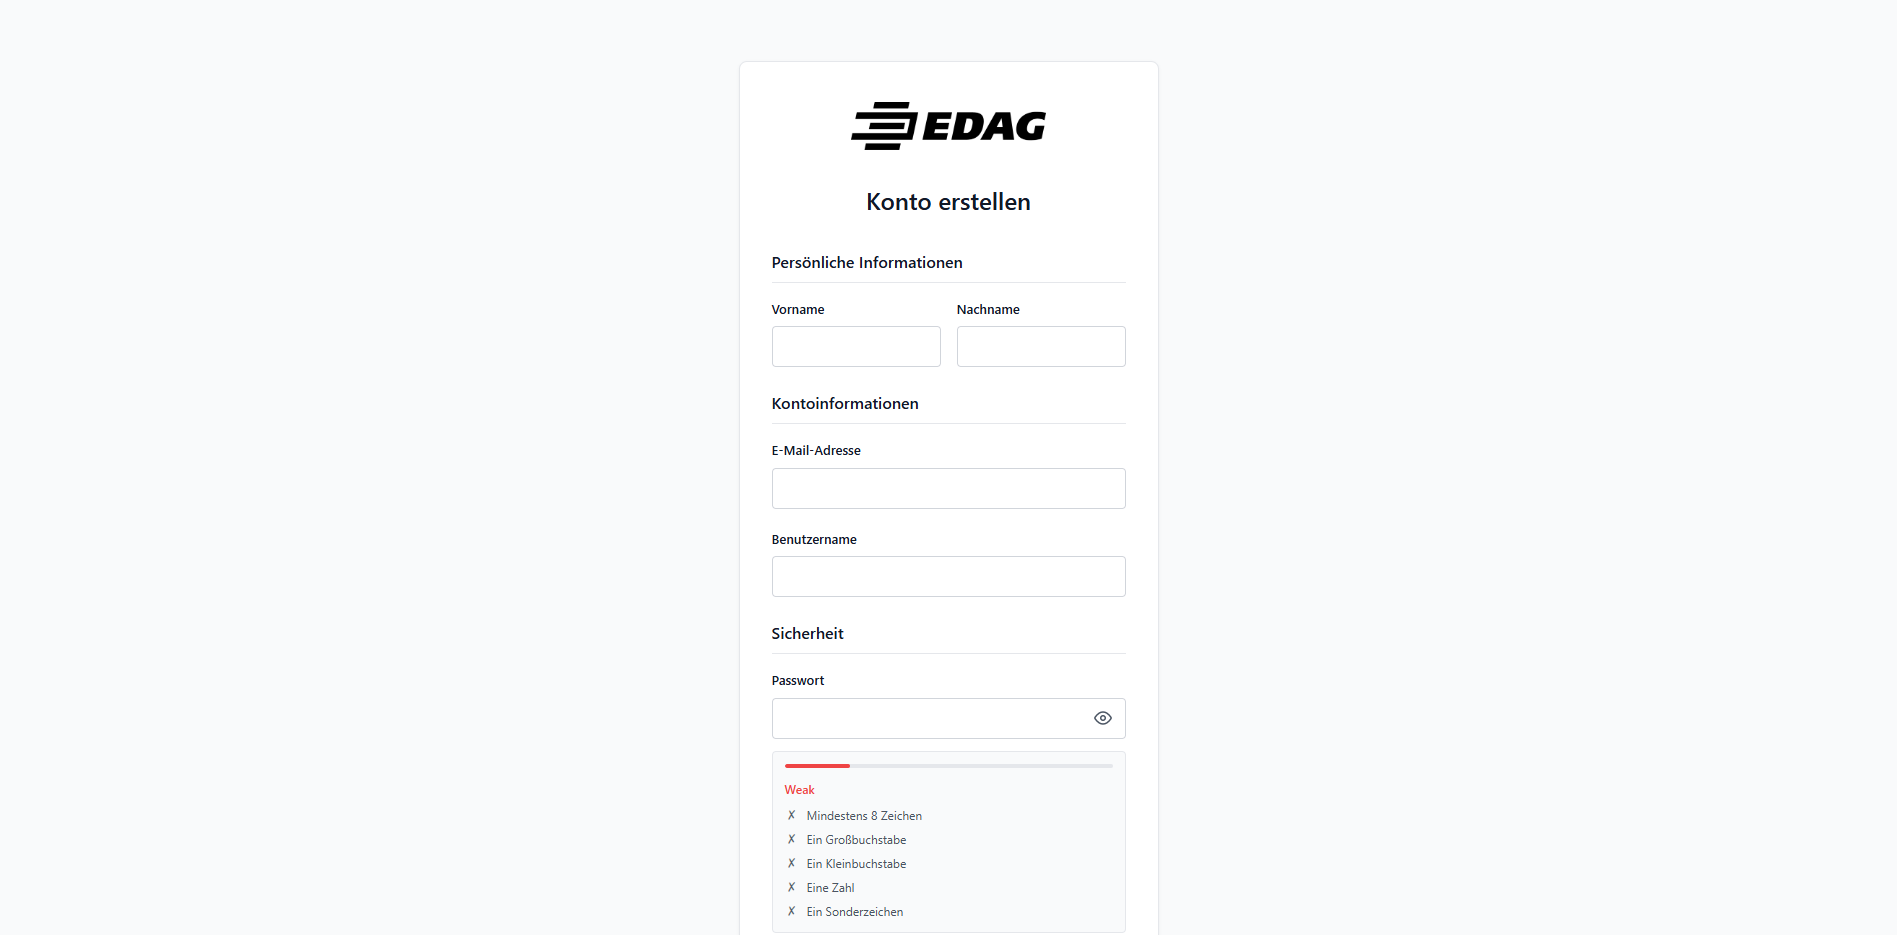
\includegraphics[width=0.9\textwidth]{references/ui-login-2.png}
\caption{Keycloak-Authentifizierungsmaske}
\label{fig:ui_login_2}
\end{figure}

\begin{figure}[H]
\centering
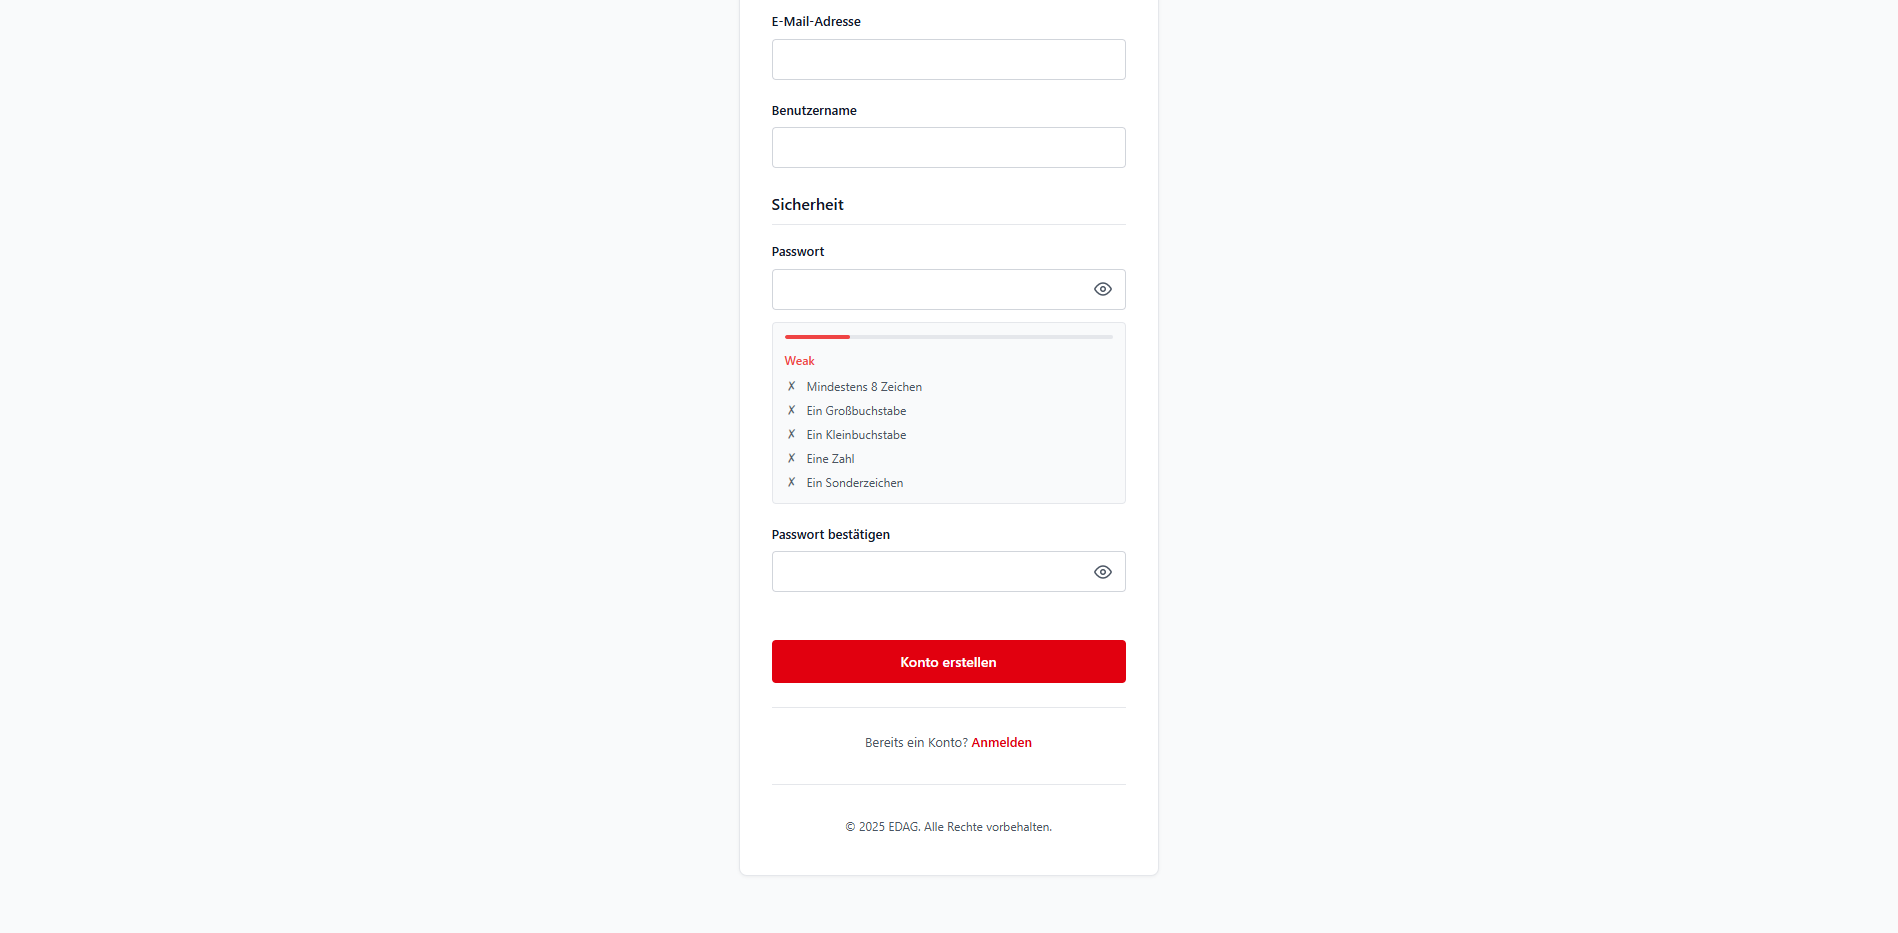
\includegraphics[width=0.9\textwidth]{references/ui-login-3.png}
\caption{Login-Erfolgsmeldung und Weiterleitung}
\label{fig:ui_login_3}
\end{figure}

\begin{figure}[H]
\centering
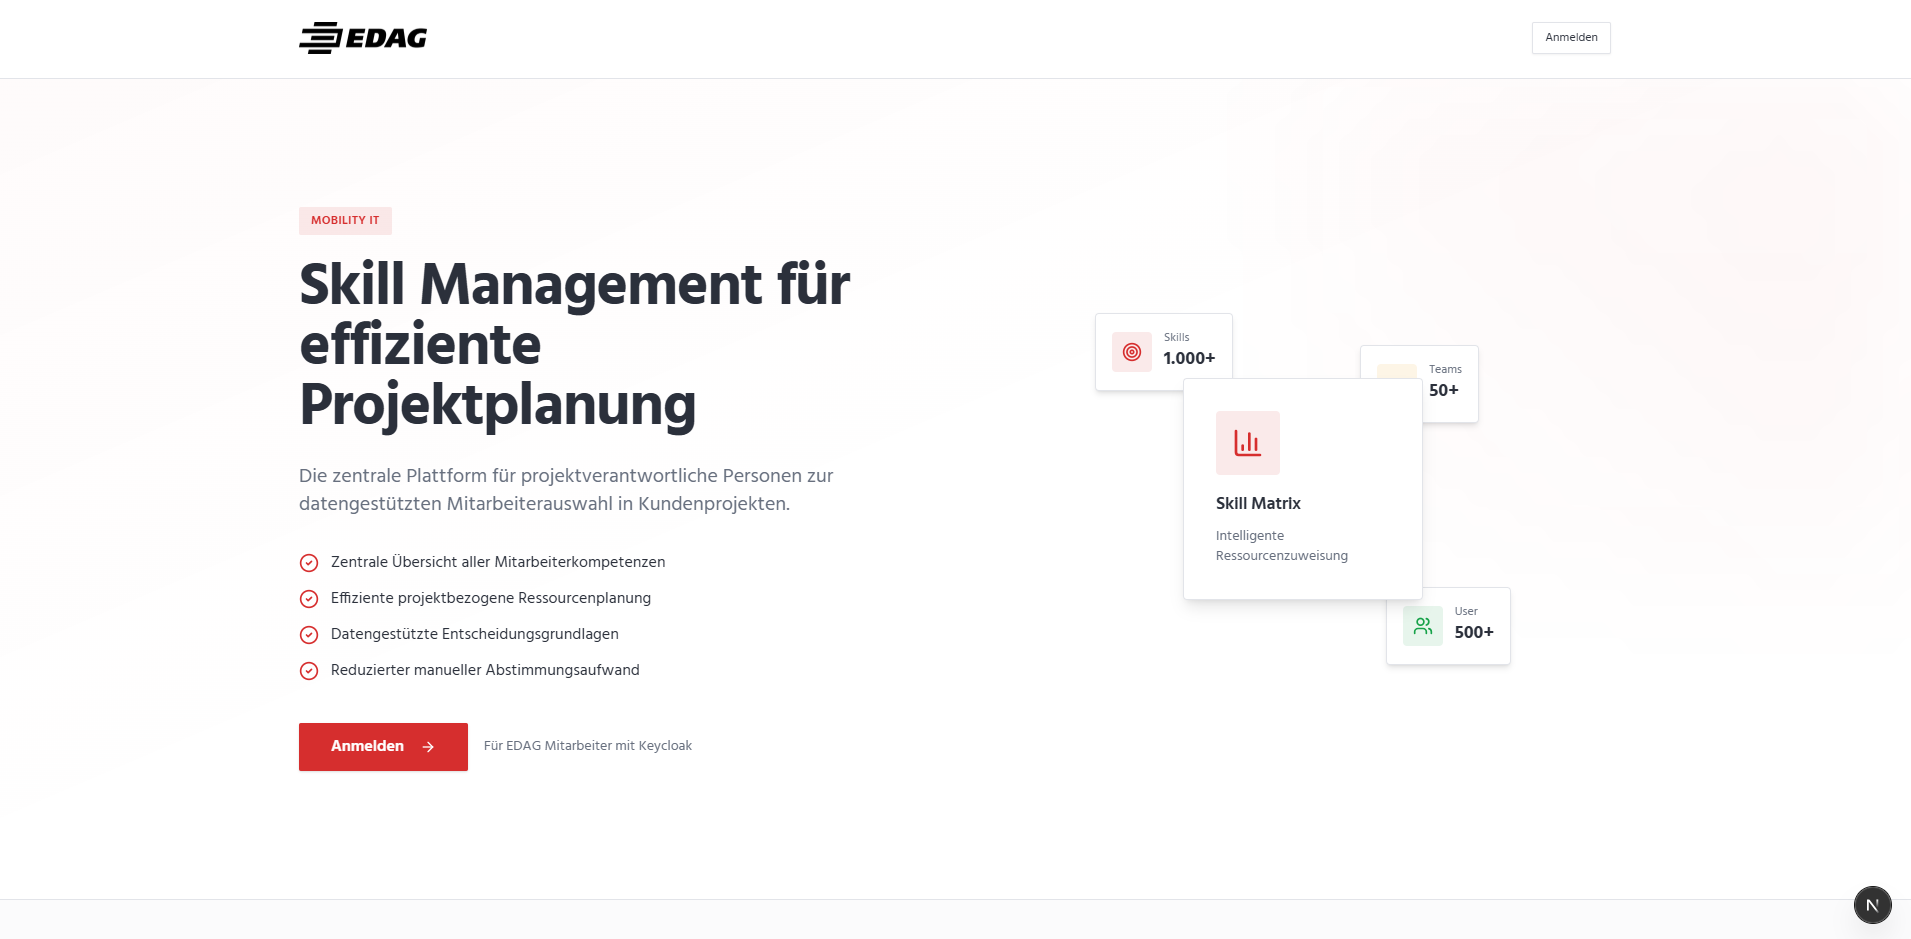
\includegraphics[width=0.9\textwidth]{references/ui-welcome-1.png}
\caption{Welcome-Seite: Erste Schritte nach Registrierung}
\label{fig:ui_welcome_1}
\end{figure}

\begin{figure}[H]
\centering
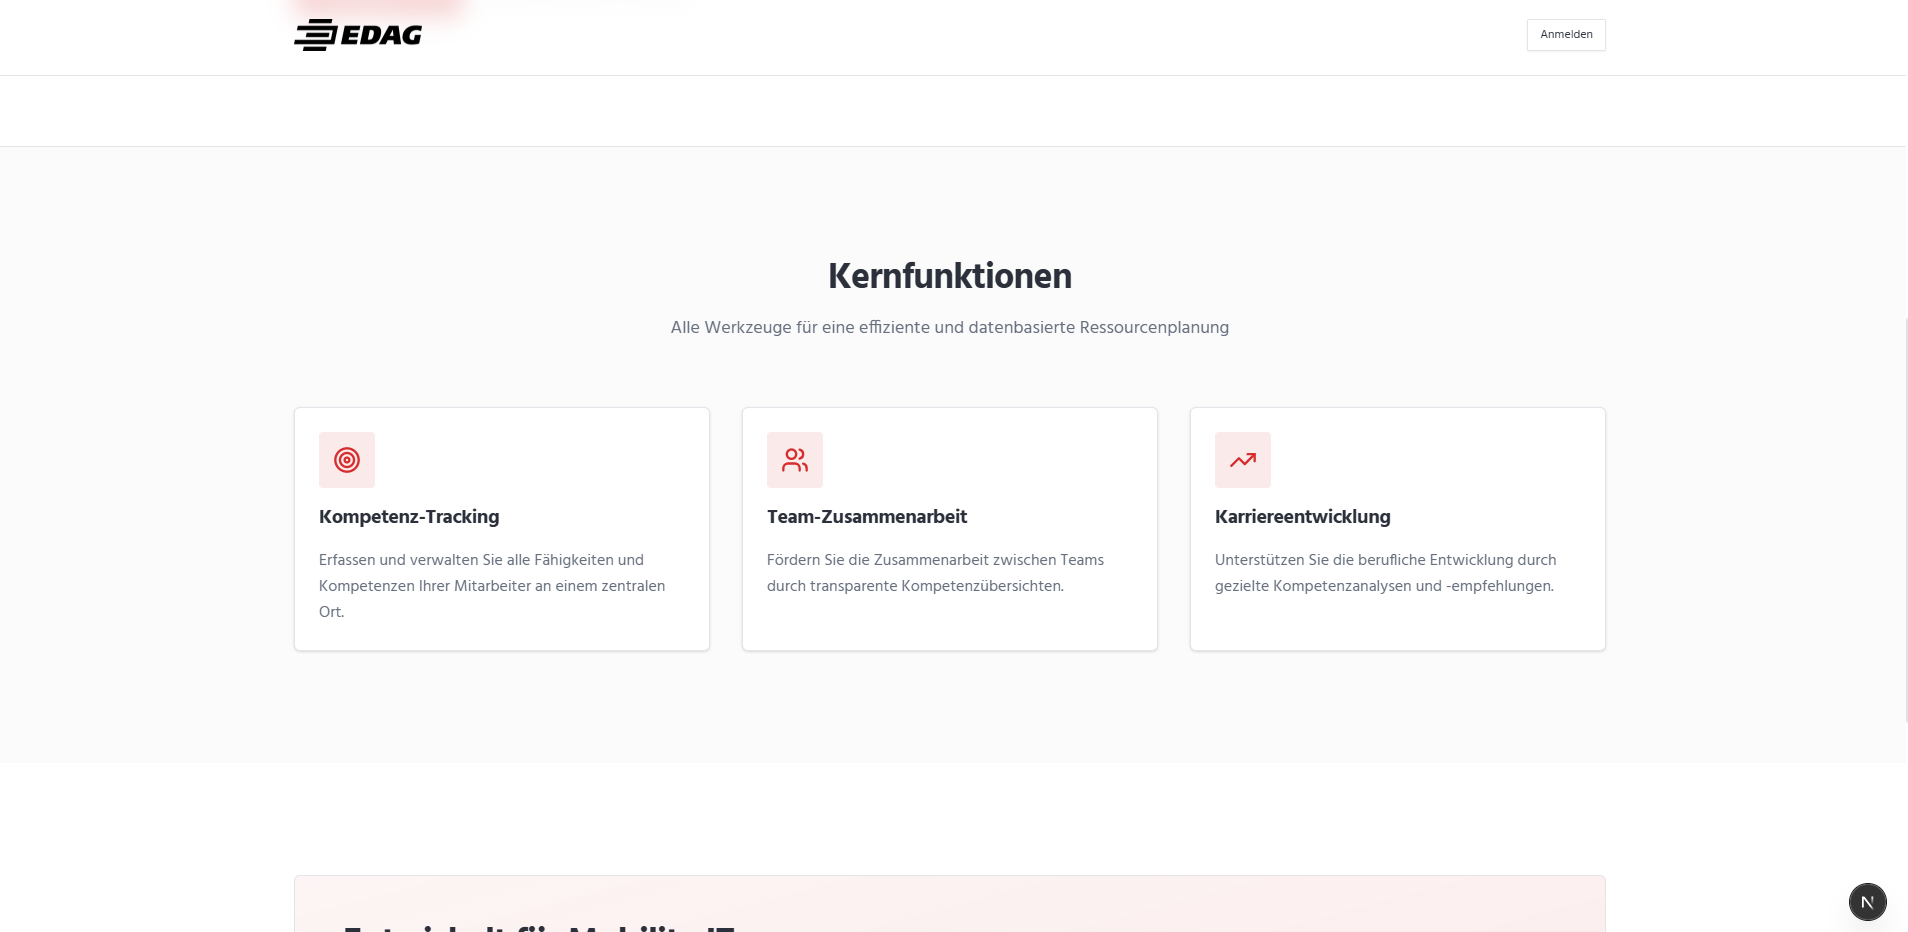
\includegraphics[width=0.9\textwidth]{references/ui-welcome-2.png}
\caption{Welcome-Seite: Profilkonfiguration}
\label{fig:ui_welcome_2}
\end{figure}

\begin{figure}[H]
\centering
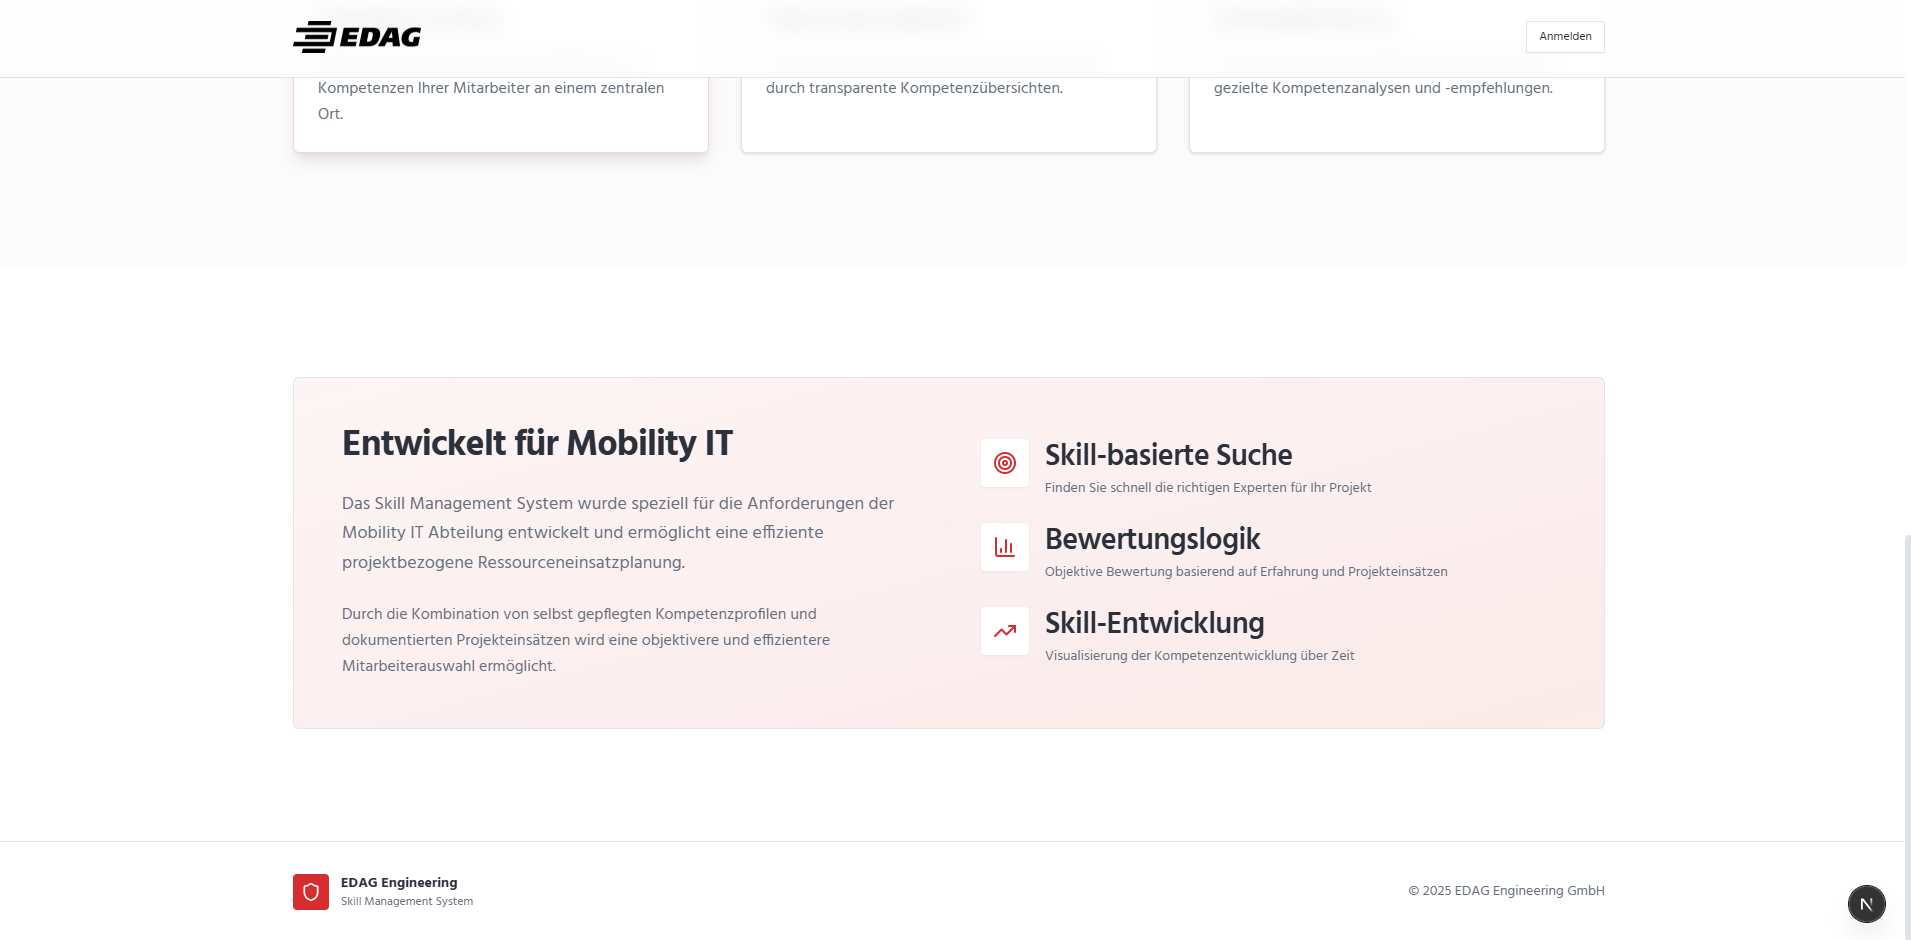
\includegraphics[width=0.9\textwidth]{references/ui-welcome-3.png}
\caption{Welcome-Seite: Skill-Auswahl}
\label{fig:ui_welcome_3}
\end{figure}

\subsubsection{Dashboard und Home}

\begin{figure}[H]
\centering
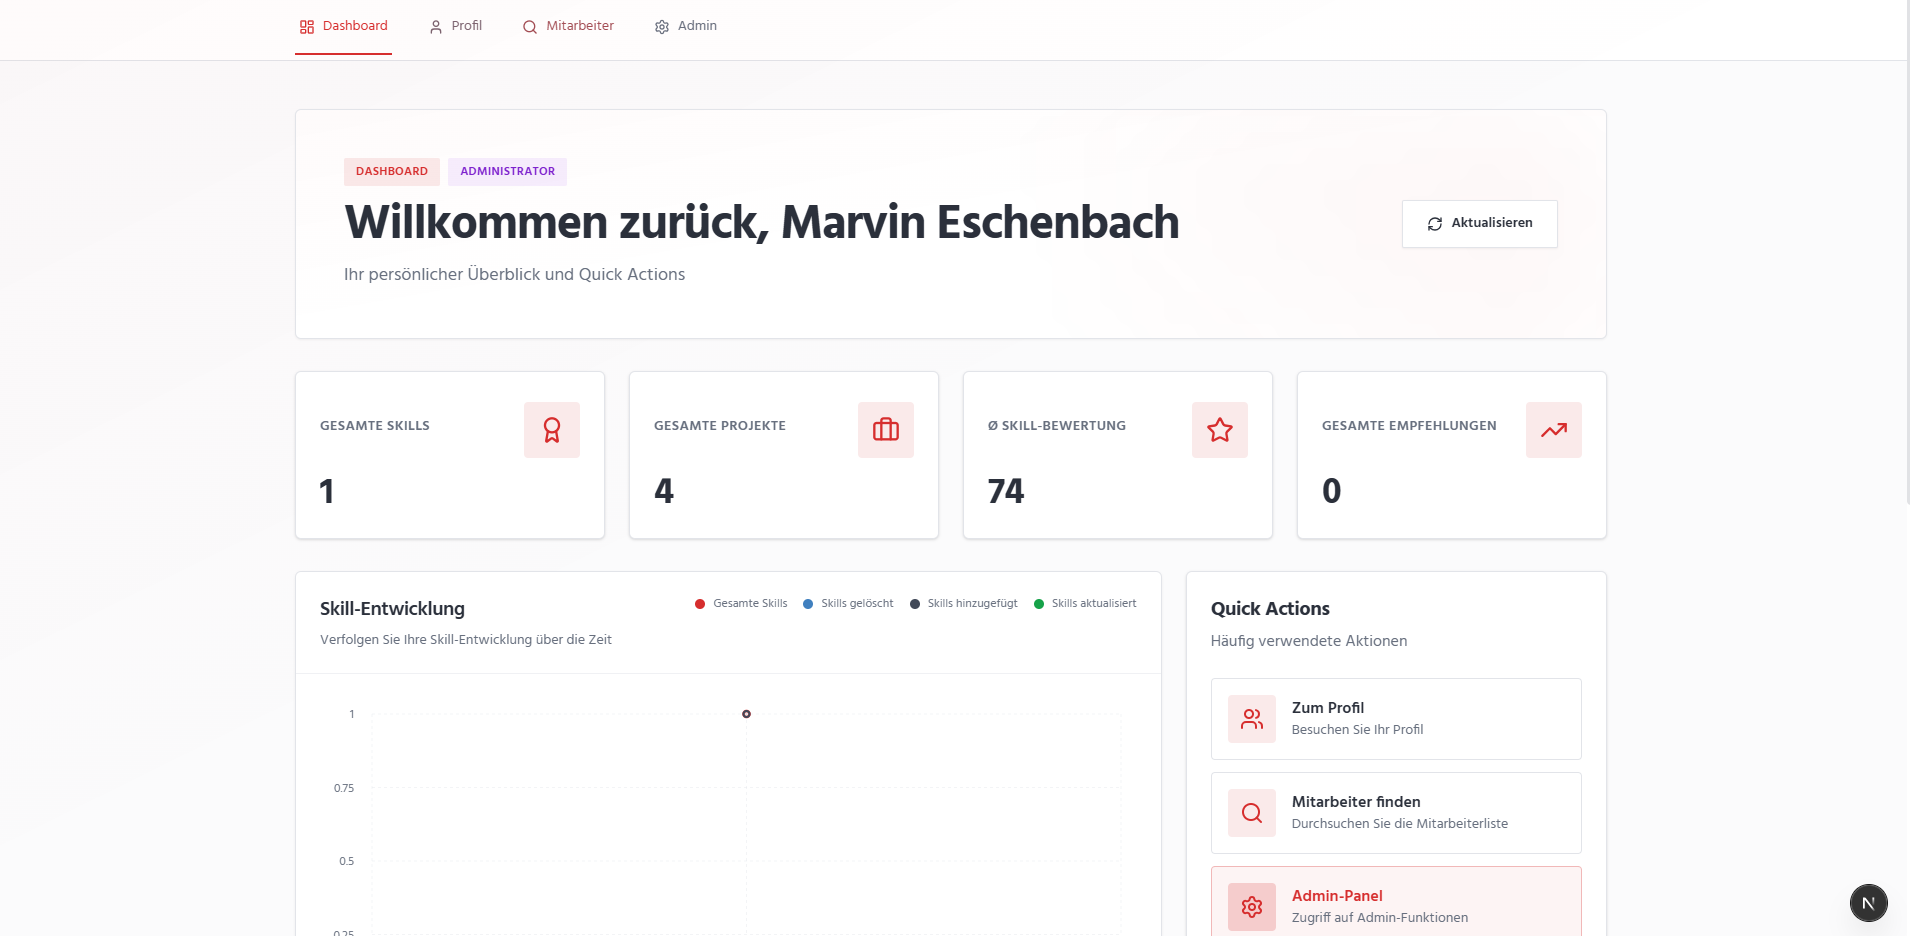
\includegraphics[width=\textwidth]{references/ui-home-1.png}
\caption{Dashboard-Übersicht mit personalisierten Kennzahlen}
\label{fig:ui_home_1}
\end{figure}

\begin{figure}[H]
\centering
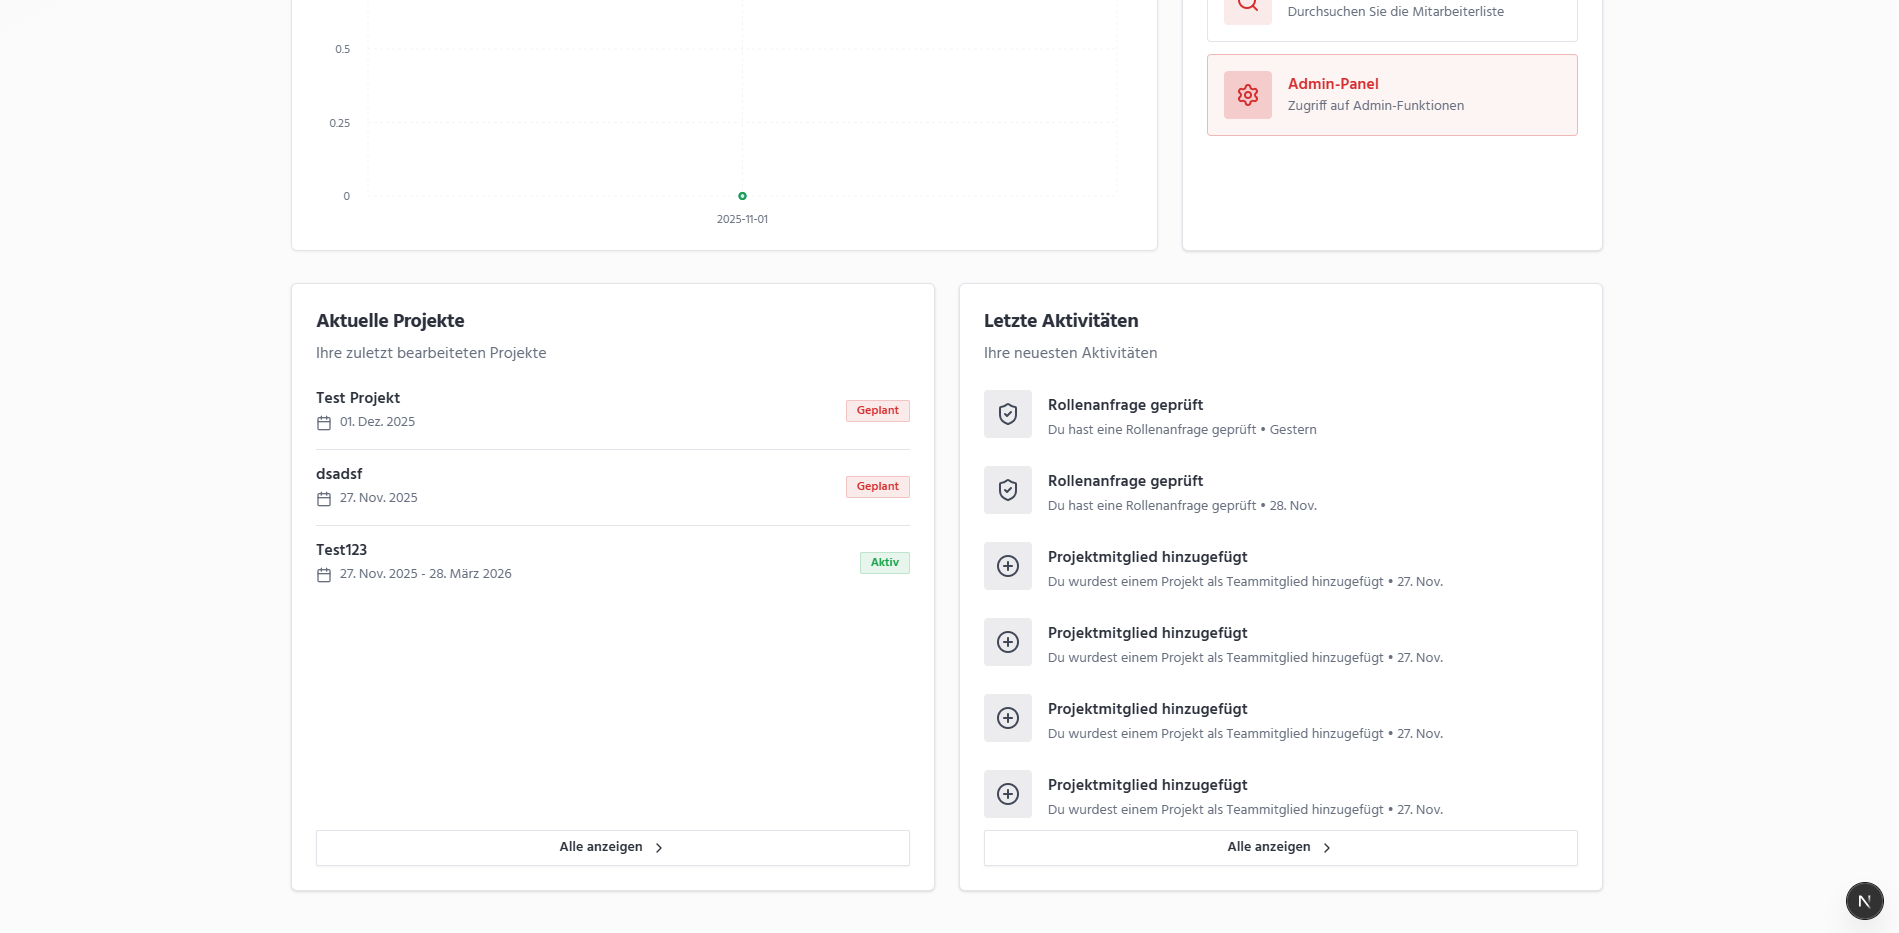
\includegraphics[width=\textwidth]{references/ui-home-2.png}
\caption{Dashboard mit Skill-Entwicklungstrends}
\label{fig:ui_home_2}
\end{figure}

\subsubsection{Profilverwaltung}

\begin{figure}[H]
\centering
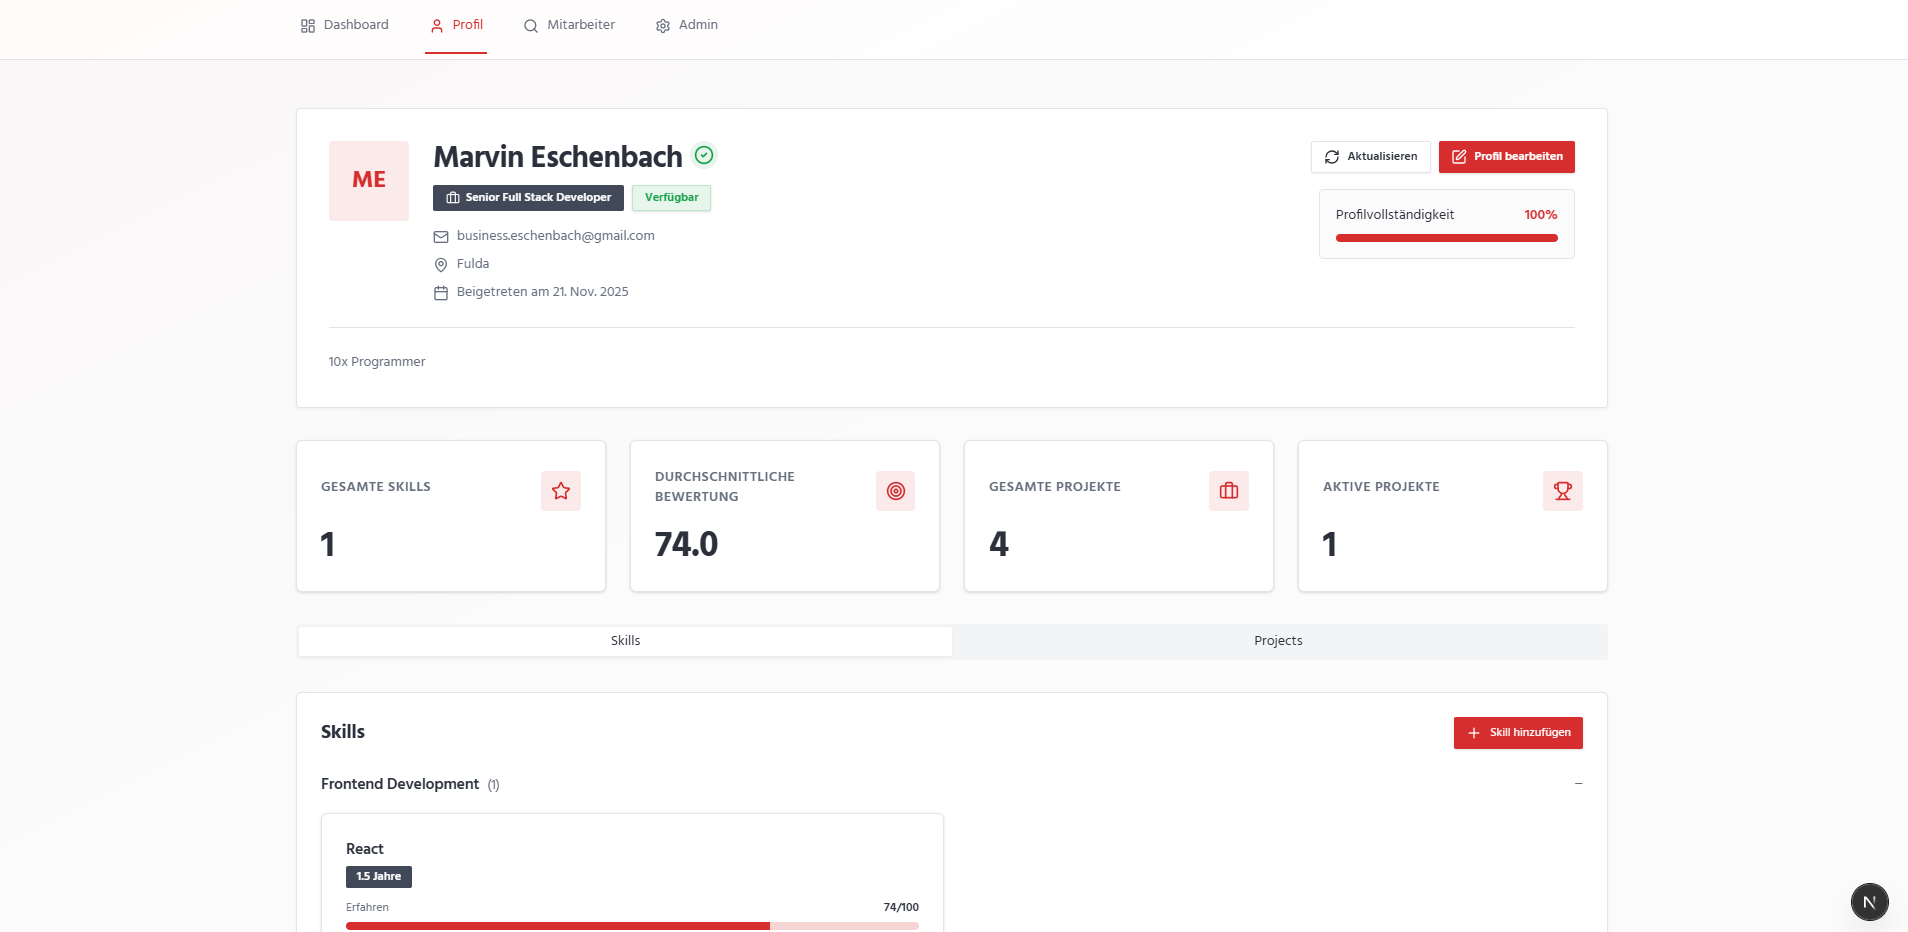
\includegraphics[width=\textwidth]{references/ui-profile-1.png}
\caption{Profil-Bearbeitung: Persönliche Daten und Skills}
\label{fig:ui_profile_1}
\end{figure}

\begin{figure}[H]
\centering
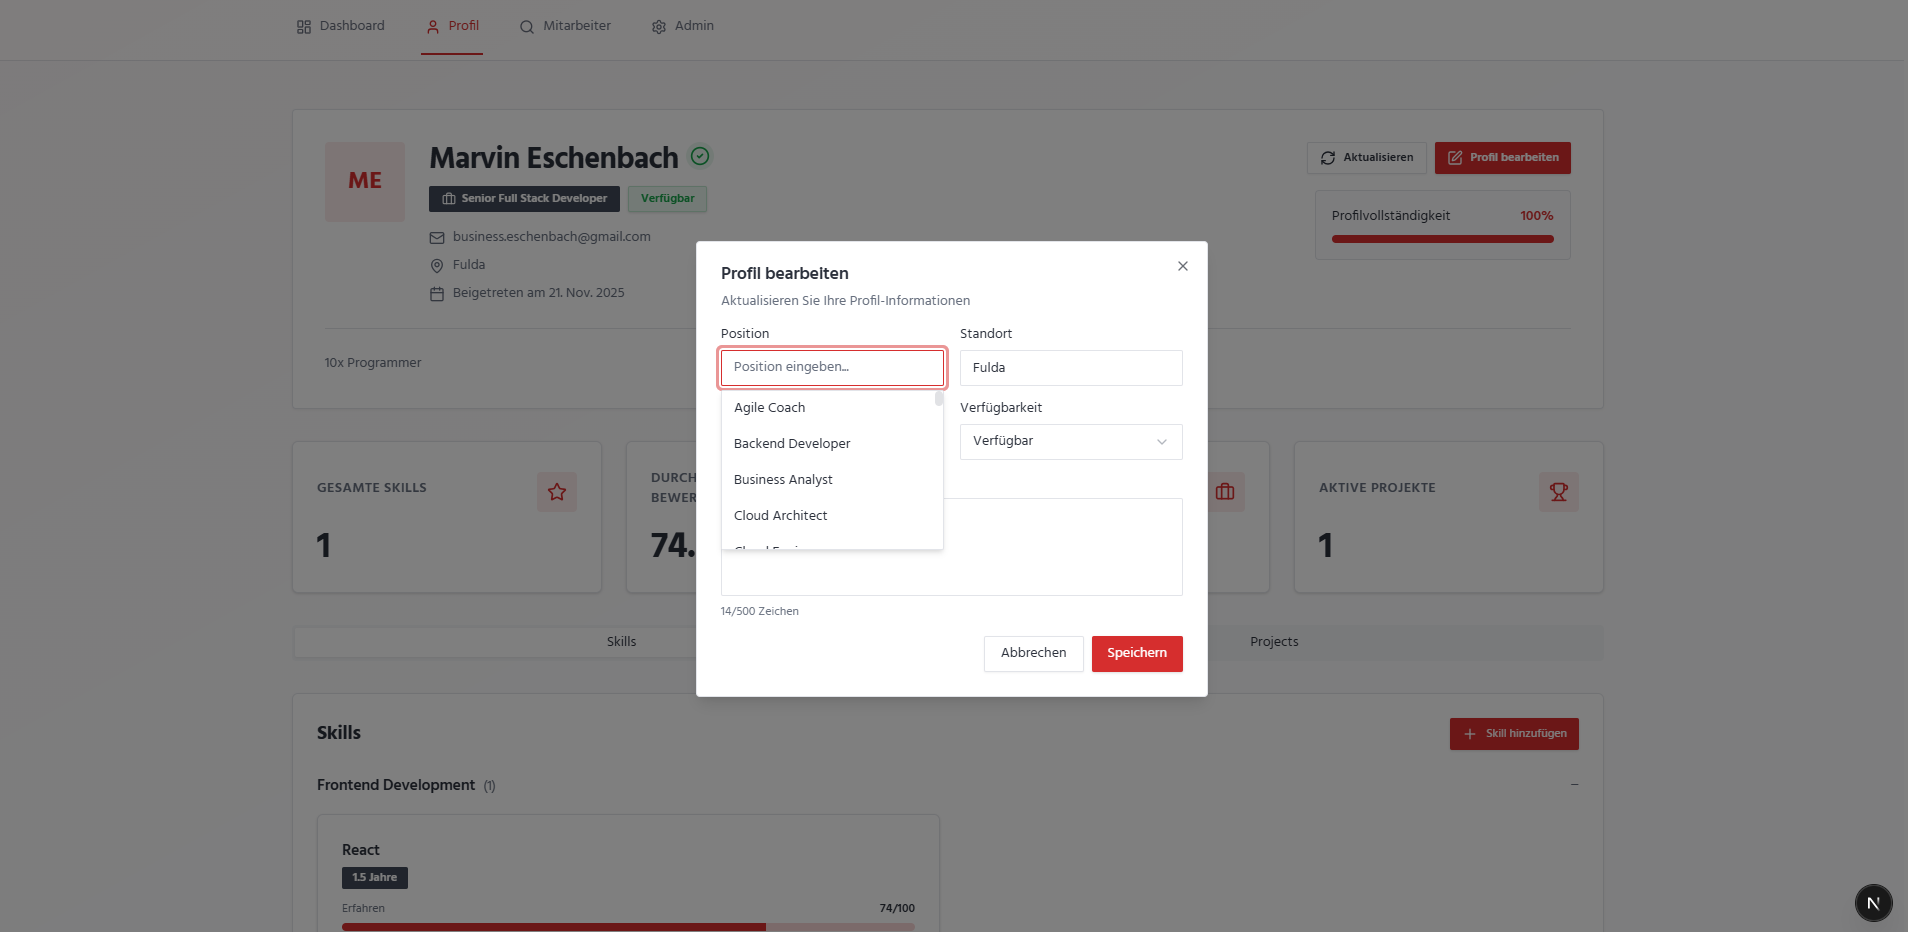
\includegraphics[width=\textwidth]{references/ui-profile-2.png}
\caption{Profil-Ansicht: Skill-Matrix mit Proficiency-Scores}
\label{fig:ui_profile_2}
\end{figure}

\subsubsection{Mitarbeiter- und Projektsuche}

\begin{figure}[H]
\centering
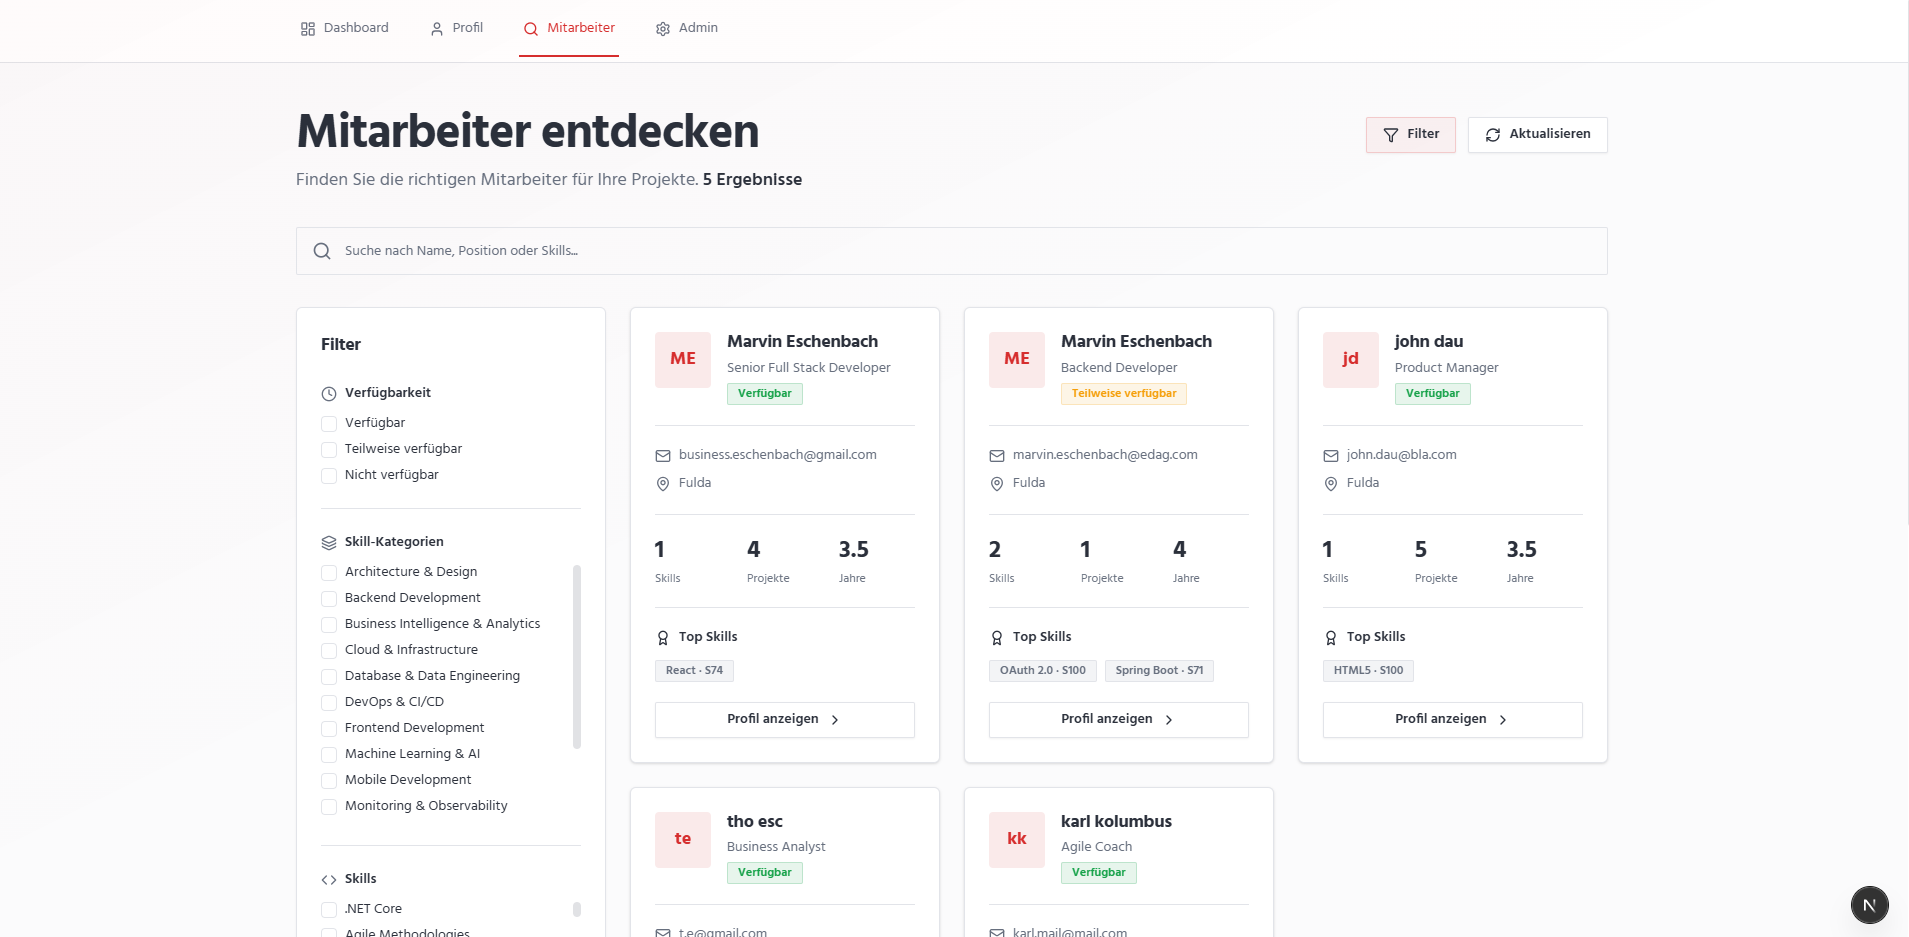
\includegraphics[width=\textwidth]{references/ui-employee-1.png}
\caption{Mitarbeitersuche mit Skill-basierten Filtern}
\label{fig:ui_employee_1}
\end{figure}

\begin{figure}[H]
\centering
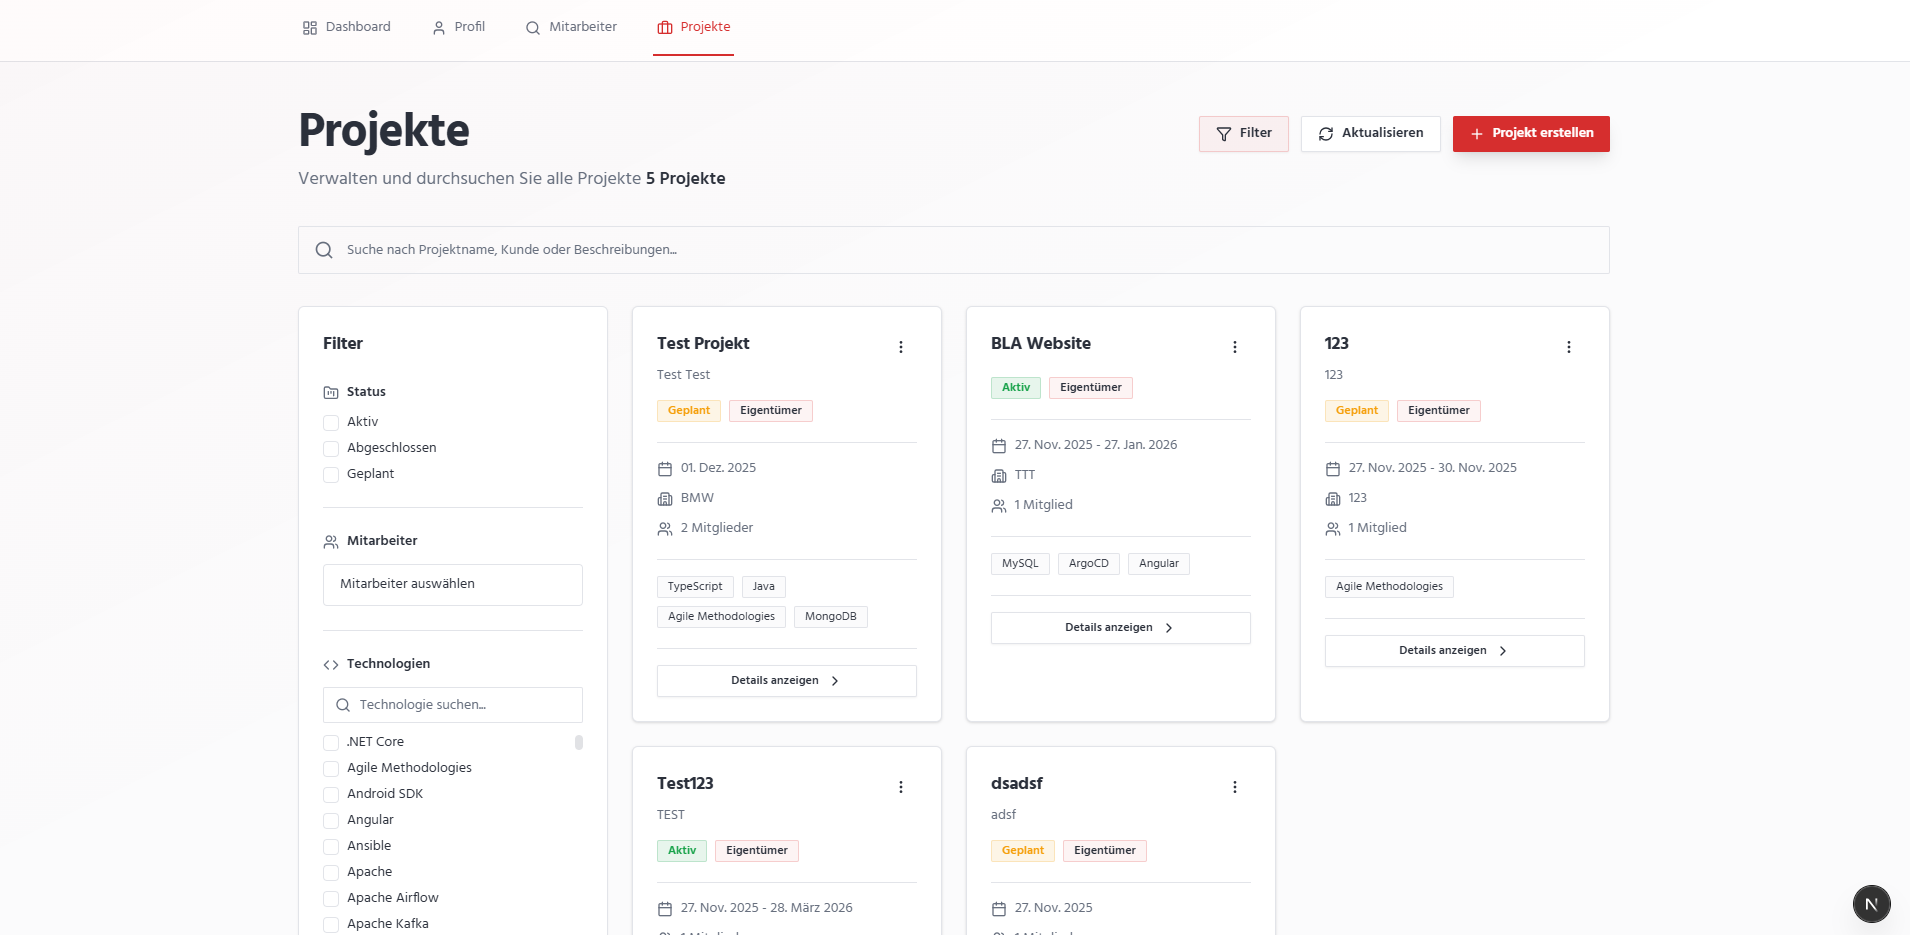
\includegraphics[width=\textwidth]{references/ui-projects-1.png}
\caption{Projektübersicht mit Status-Filter}
\label{fig:ui_projects_1}
\end{figure}

\begin{figure}[H]
\centering
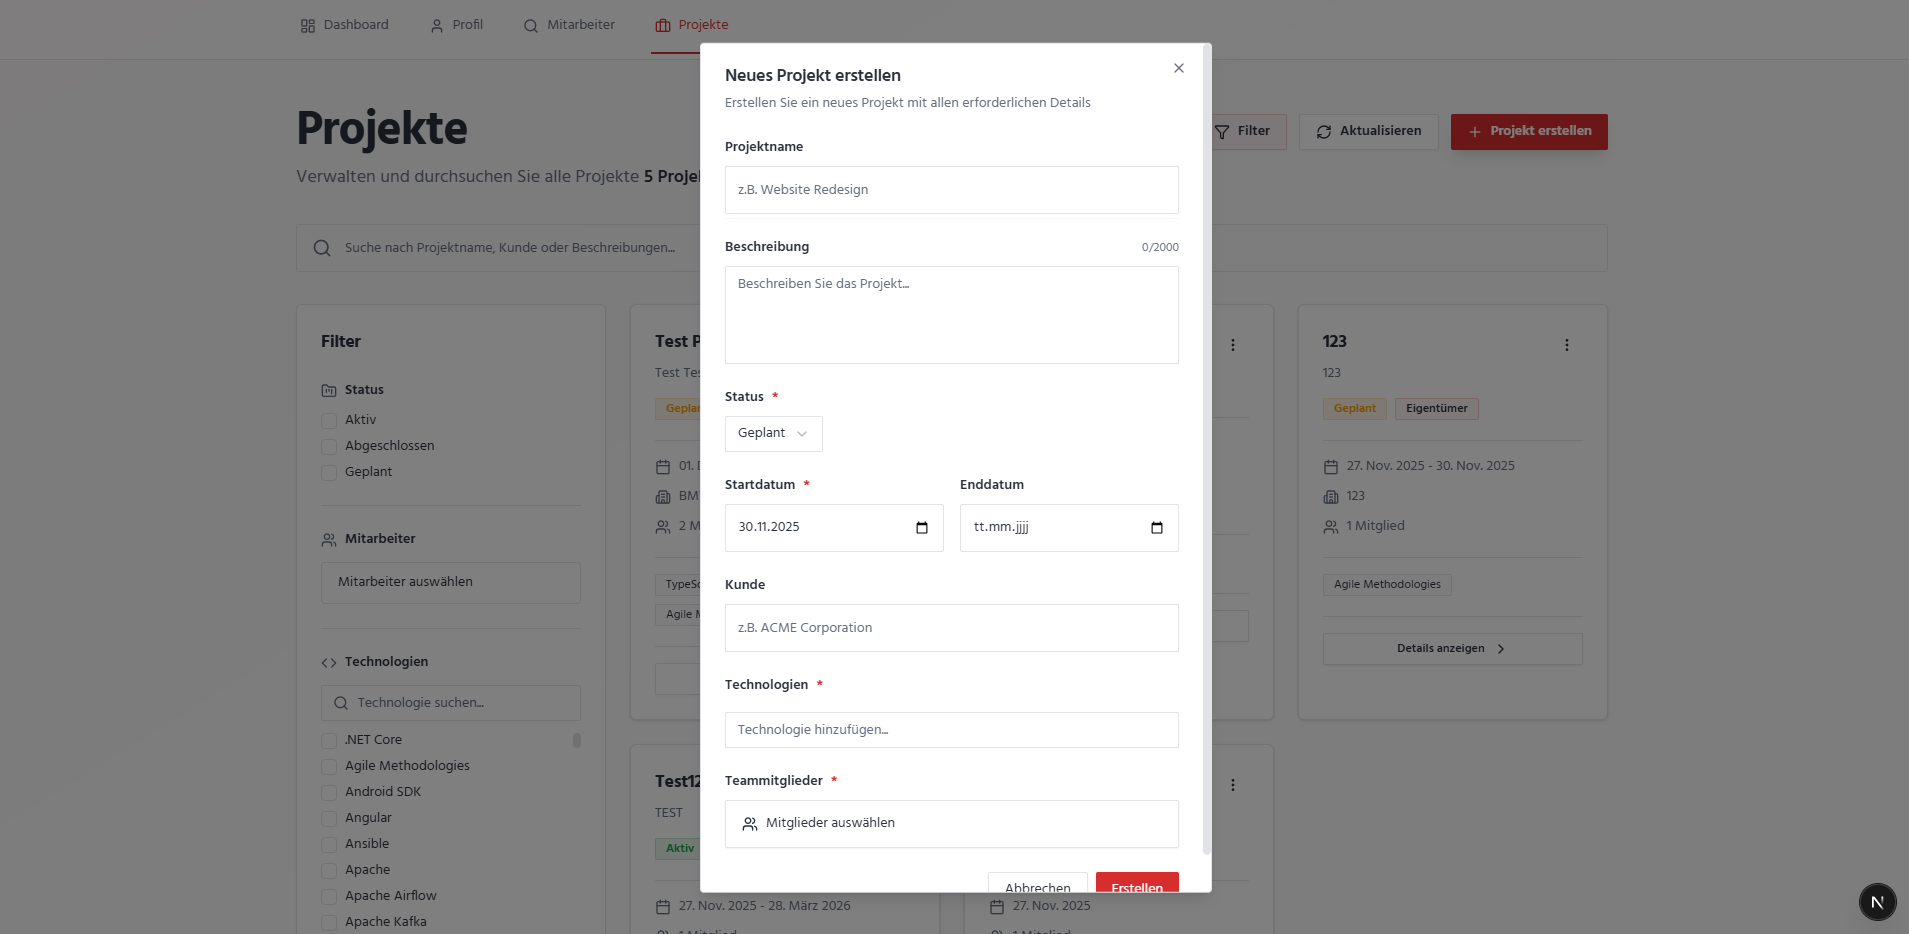
\includegraphics[width=\textwidth]{references/ui-projects-2.png}
\caption{Projekt-Detailansicht mit Team-Zusammensetzung}
\label{fig:ui_projects_2}
\end{figure}

\begin{figure}[H]
\centering
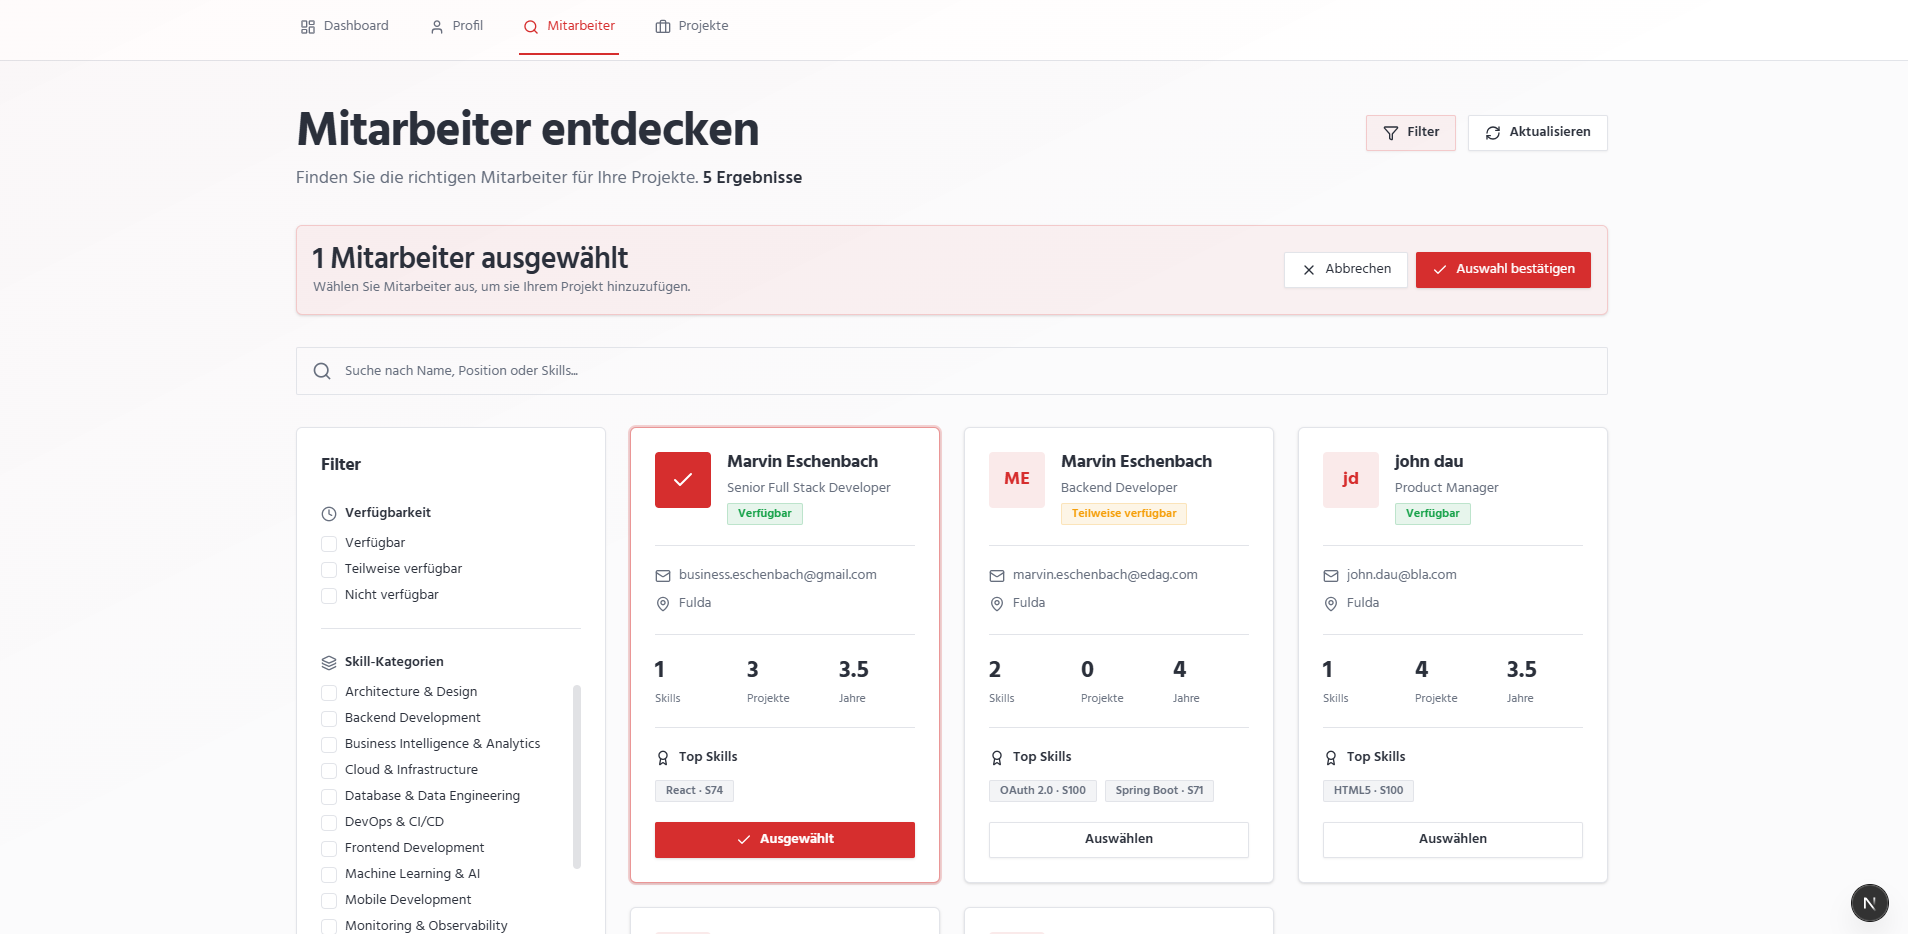
\includegraphics[width=\textwidth]{references/ui-projects-3.png}
\caption{Projekt-Erstellung: Formular für neue Projekte}
\label{fig:ui_projects_3}
\end{figure}

\begin{figure}[H]
\centering
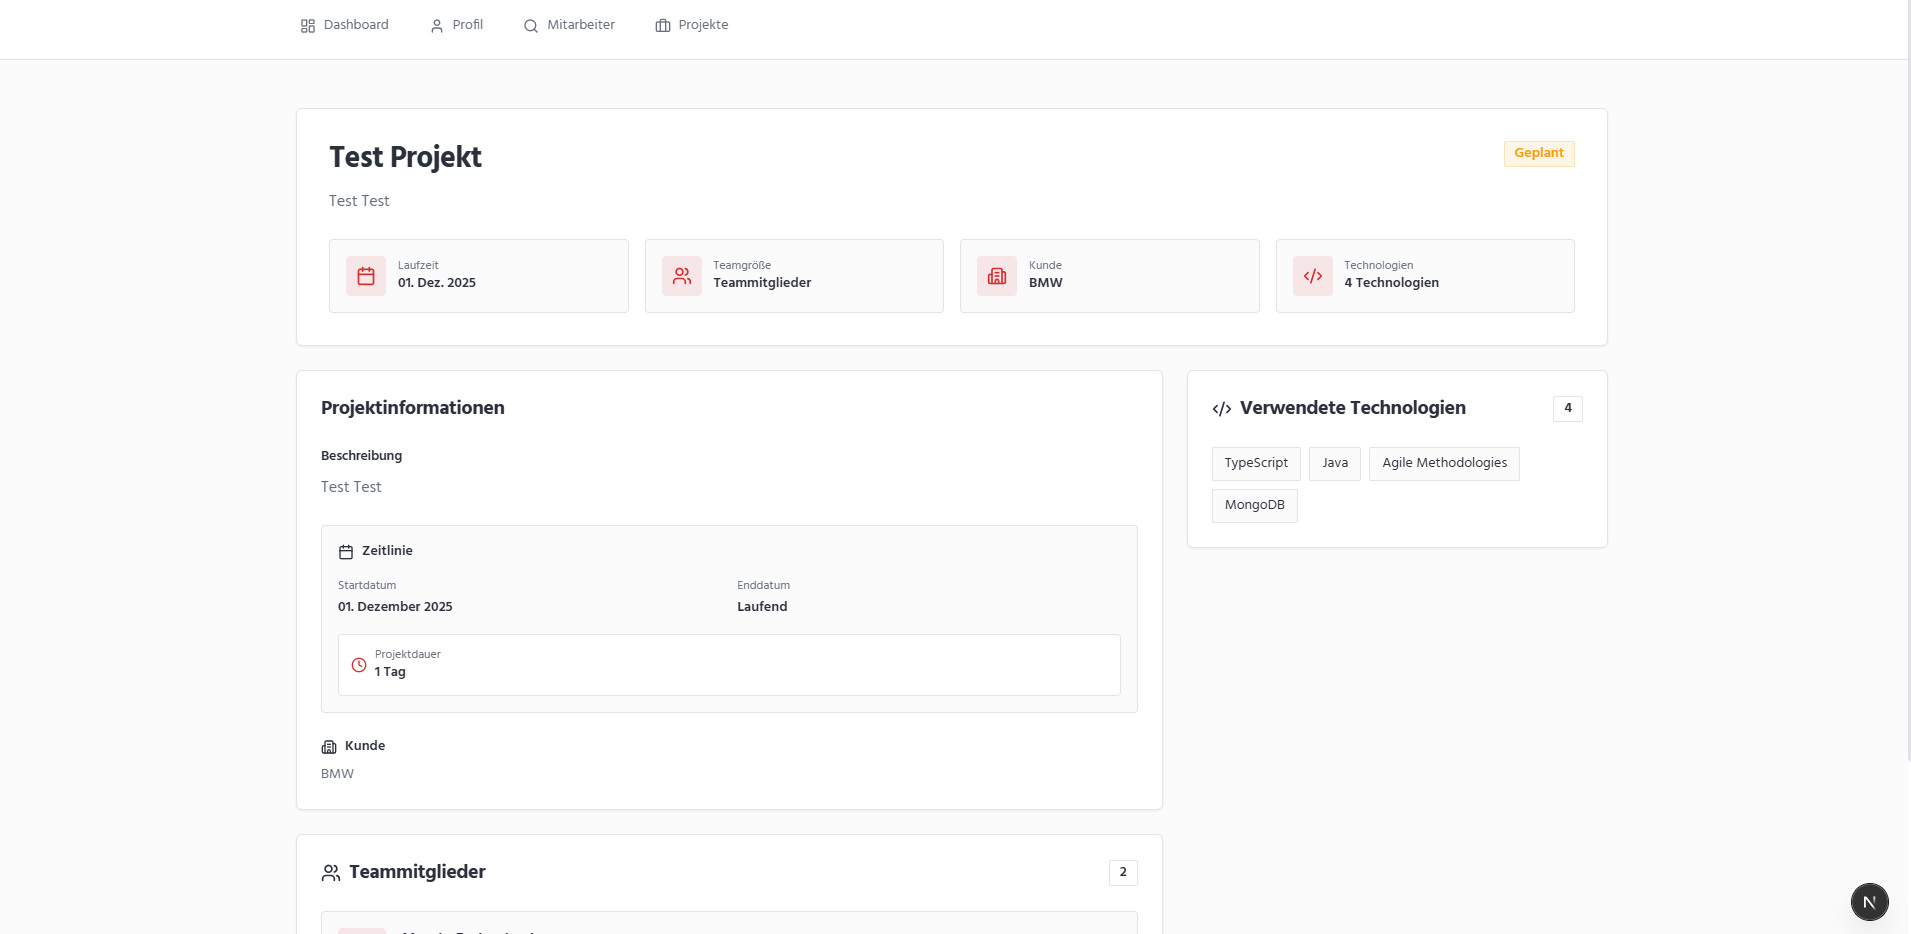
\includegraphics[width=\textwidth]{references/ui-projects-4.png}
\caption{Projekt-Team-Management: Mitglieder hinzufügen}
\label{fig:ui_projects_4}
\end{figure}

\subsubsection{Administrationsoberfläche}

\begin{figure}[H]
\centering
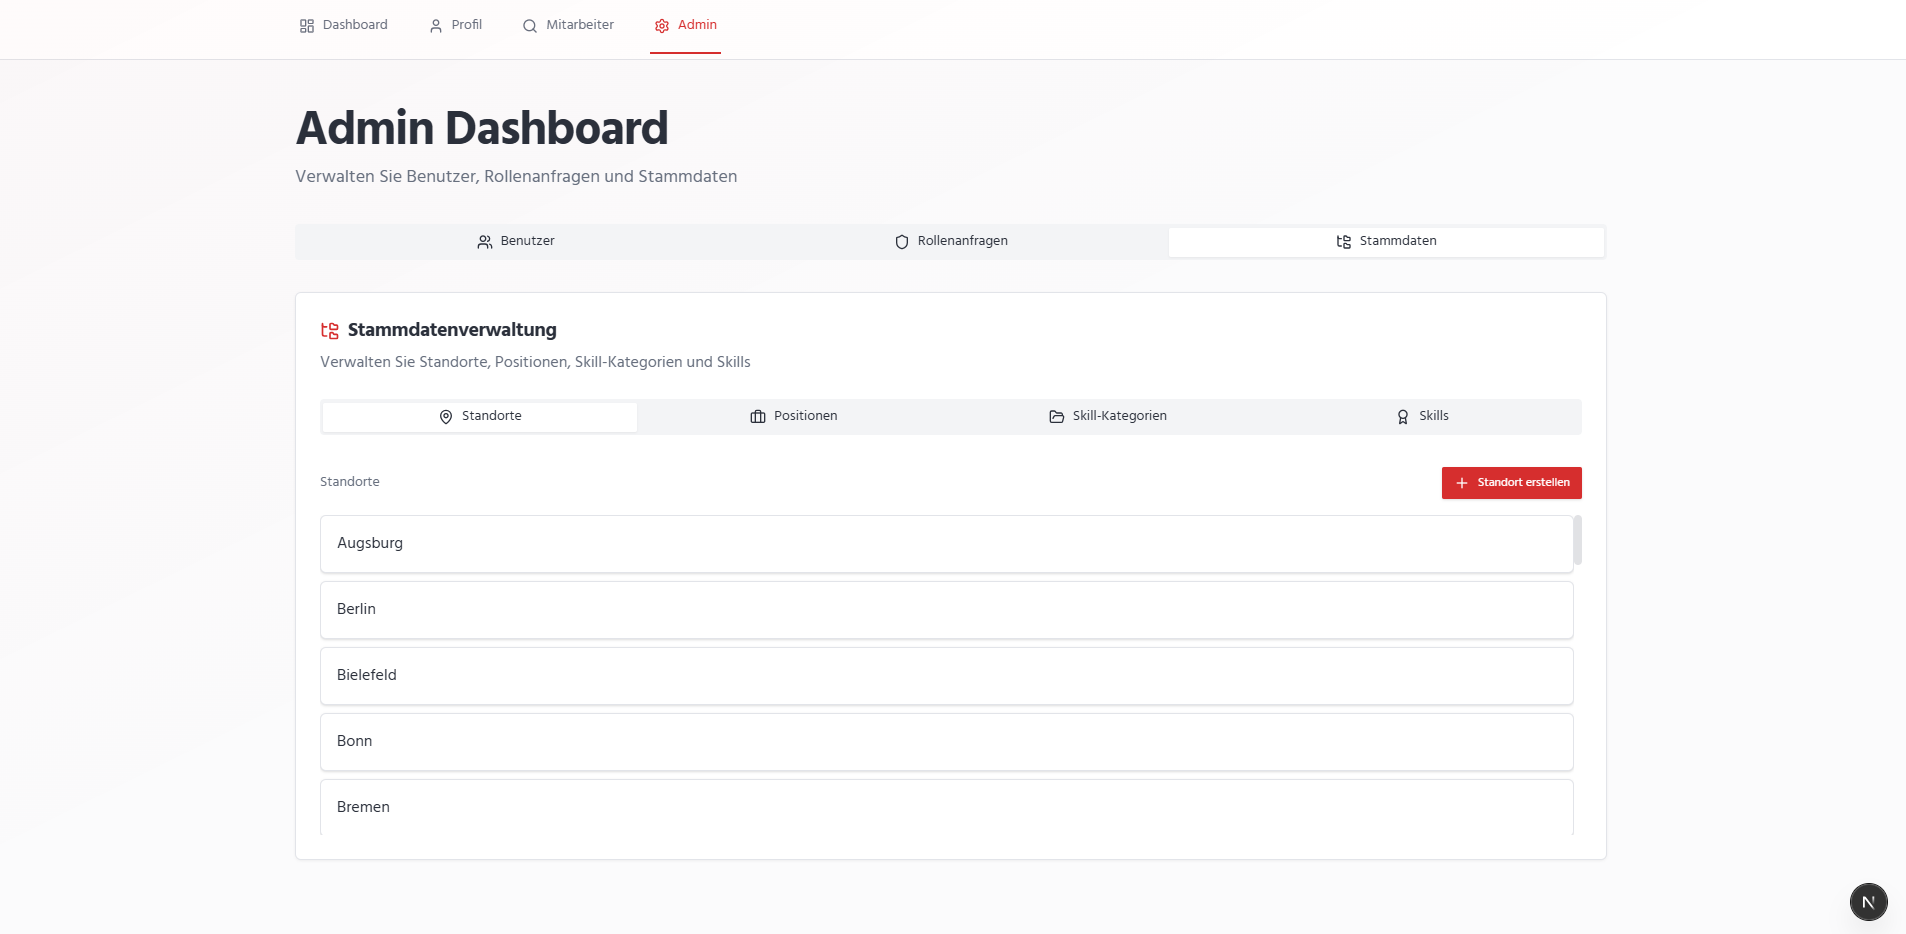
\includegraphics[width=\textwidth]{references/ui-admin-1.png}
\caption{Admin-Dashboard: Systemstatistiken und Benutzeraktivitäten}
\label{fig:ui_admin_1}
\end{figure}

\begin{figure}[H]
\centering
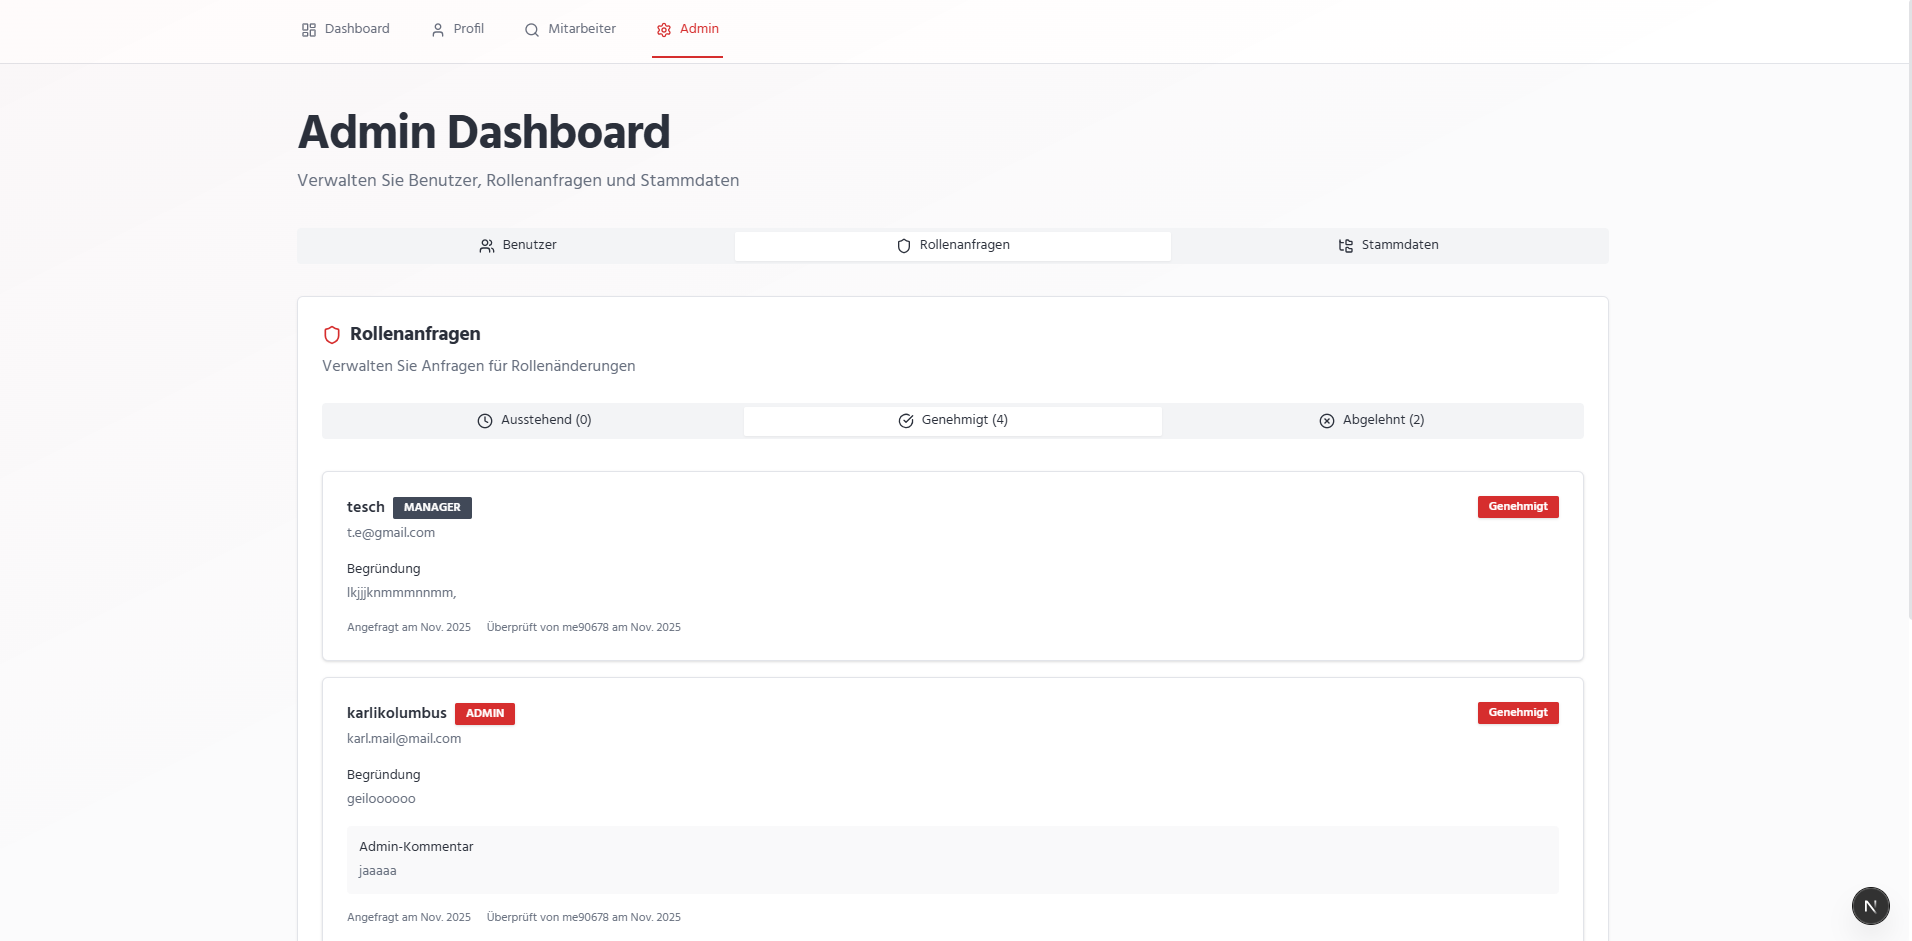
\includegraphics[width=\textwidth]{references/ui-admin-2.png}
\caption{Admin-Panel: Rollenanfragen-Verwaltung}
\label{fig:ui_admin_2}
\end{figure}

\subsubsection{UI-Mockup (Planungsphase)}

\begin{figure}[H]
\centering
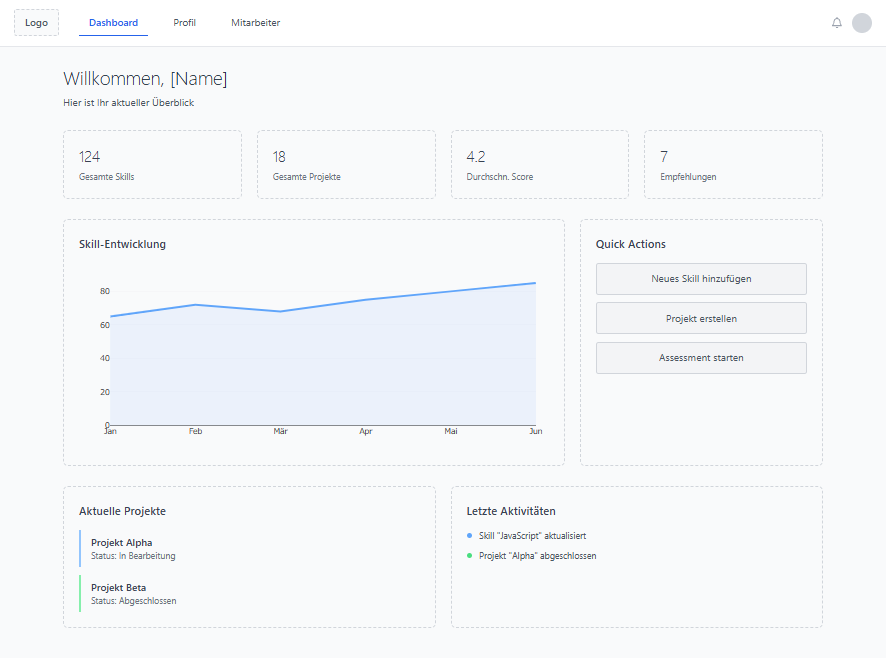
\includegraphics[width=\textwidth]{references/mockup-dashboard.png}
\caption{Initiales UI-Mockup aus der Planungsphase}
\label{fig:mockup_dashboard}
\end{figure}

\subsection{Use Cases}

\subsubsection{Übersicht der 15 implementierten Use Cases}

\begin{table}[H]
\centering
\footnotesize
\rowcolors{2}{EDAGDunkelgrau!10}{white}
\begin{tabularx}{\textwidth}{|l|X|p{2cm}|}
\hline
\rowcolor{EDAGDunkelgrau!10}
\textbf{Nr.} & \textbf{Use Case} & \textbf{Rolle} \\
\hline
UC-01 & Login über Keycloak OAuth2/OIDC & Alle \\
\hline
UC-02 & Eigenes Profil anzeigen und bearbeiten & USER \\
\hline
UC-03 & Skills hinzufügen/bearbeiten mit Proficiency Score & USER \\
\hline
UC-04 & Dashboard mit Skill-Entwicklung anzeigen & USER \\
\hline
UC-05 & Activity Feed anzeigen & USER \\
\hline
UC-06 & Mitarbeiter suchen (Multi-Filter) & USER \\
\hline
UC-07 & Projekte suchen & USER \\
\hline
UC-08 & Projekt anlegen mit Mitarbeiterauswahl & MANAGER \\
\hline
UC-09 & Projekt bearbeiten/Teammitglieder ändern & MANAGER \\
\hline
UC-10 & Projektdetails anzeigen & MANAGER \\
\hline
UC-11 & Rollenanfrage stellen (USER→MANAGER) & USER \\
\hline
UC-12 & Rollenanfrage genehmigen/ablehnen & ADMIN \\
\hline
UC-13 & Benutzerverwaltung (Rollenzuweisung) & ADMIN \\
\hline
UC-14 & Stammdaten verwalten (Skills, Kategorien) & ADMIN \\
\hline
UC-15 & Standorte verwalten & ADMIN \\
\hline
\end{tabularx}
\caption{Übersicht der 15 implementierten Use Cases}
\label{tab:use_cases}
\end{table}

\subsection{Benutzer- und Entwicklerdokumentation}

\begin{figure}[H]
\centering
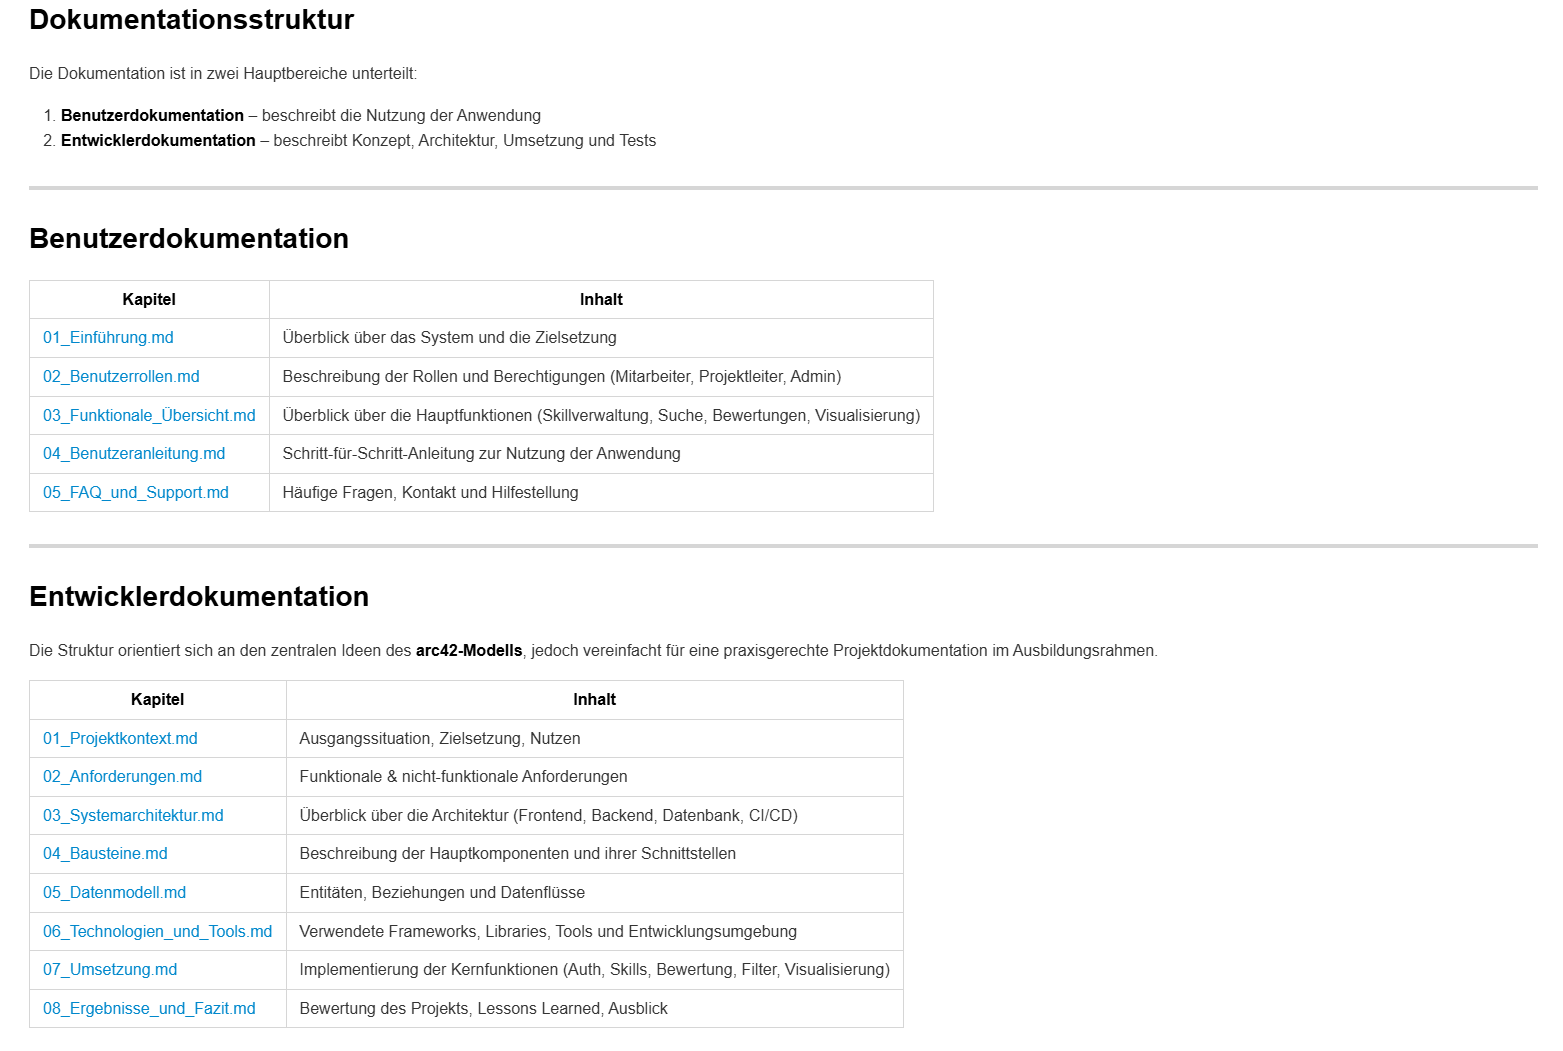
\includegraphics[width=\textwidth]{references/doc-1.png}
\caption{Benutzer- und Entwicklerdokumentation: Deckblatt der Benutzerdokumentation}
\label{fig:doc_user_guide}
\end{figure}

\begin{figure}[H]
\centering
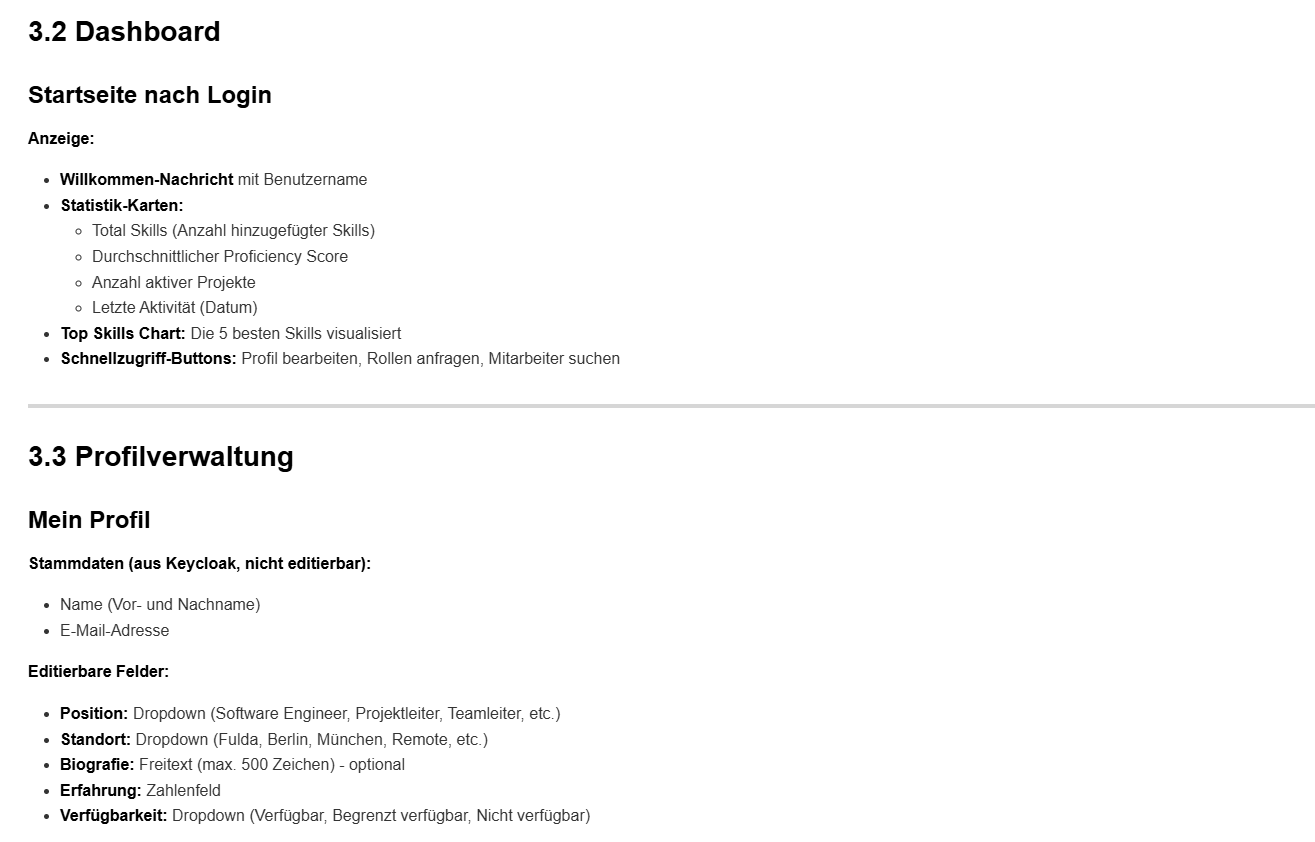
\includegraphics[width=\textwidth]{references/doc-2.png}
\caption{Benutzer- und Entwicklerdokumentation: Auszug aus der funktionalen Übersicht (Kapitel 3)}
\label{fig:doc_functional_overview}
\end{figure}

\begin{figure}[H]
\centering
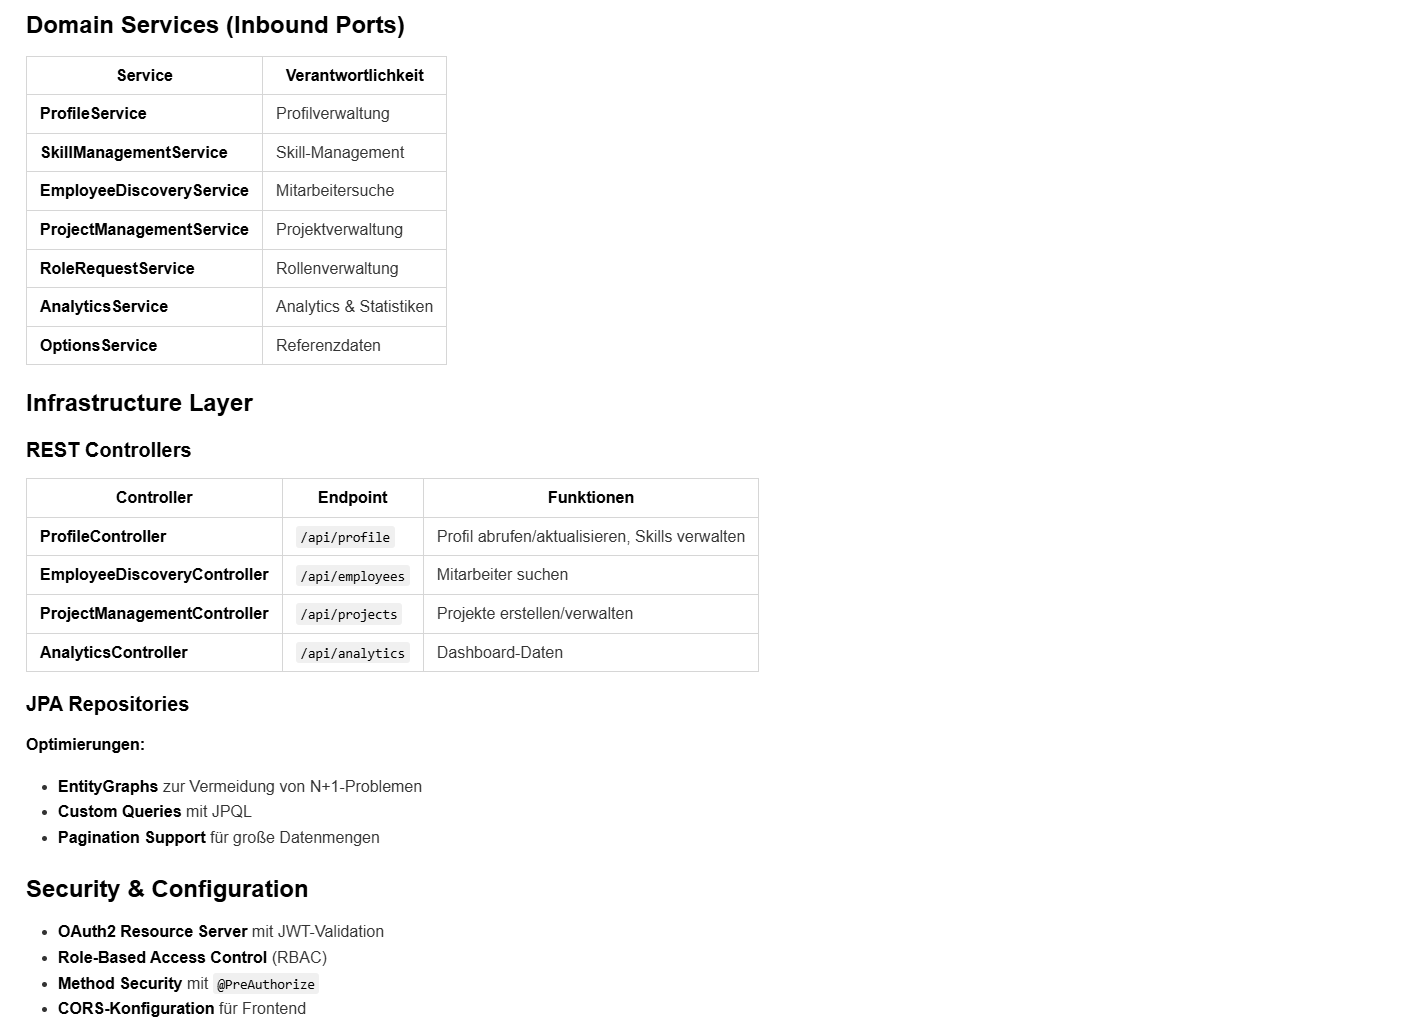
\includegraphics[width=\textwidth]{references/doc-3.png}
\caption{Benutzer- und Entwicklerdokumentation: Auszug aus der Architekturübersicht (Kapitel 4 - Bausteine)}
\label{fig:doc_architecture_blocks}
\end{figure}

Die Abbildungen~\ref{fig:doc_user_guide} bis~\ref{fig:doc_architecture_blocks} zeigen exemplarische Auszüge aus der erstellten Benutzer- und Entwicklerdokumentation, die eine umfassende Beschreibung aller Systemfunktionen, der technischen Architektur und der Deployment-Prozesse enthält.

\subsection{API-Dokumentation}
\label{sec:api_documentation}

Die REST-API des Skill Management Systems folgt RESTful-Prinzipien und ist vollständig mit OpenAPI 3.0 dokumentiert. Die API umfasst 7 Hauptbereiche mit insgesamt über 30 Endpunkten für Profilverwaltung, Mitarbeitersuche, Projektmanagement, Administration und Analytics.

\begin{figure}[H]
\centering
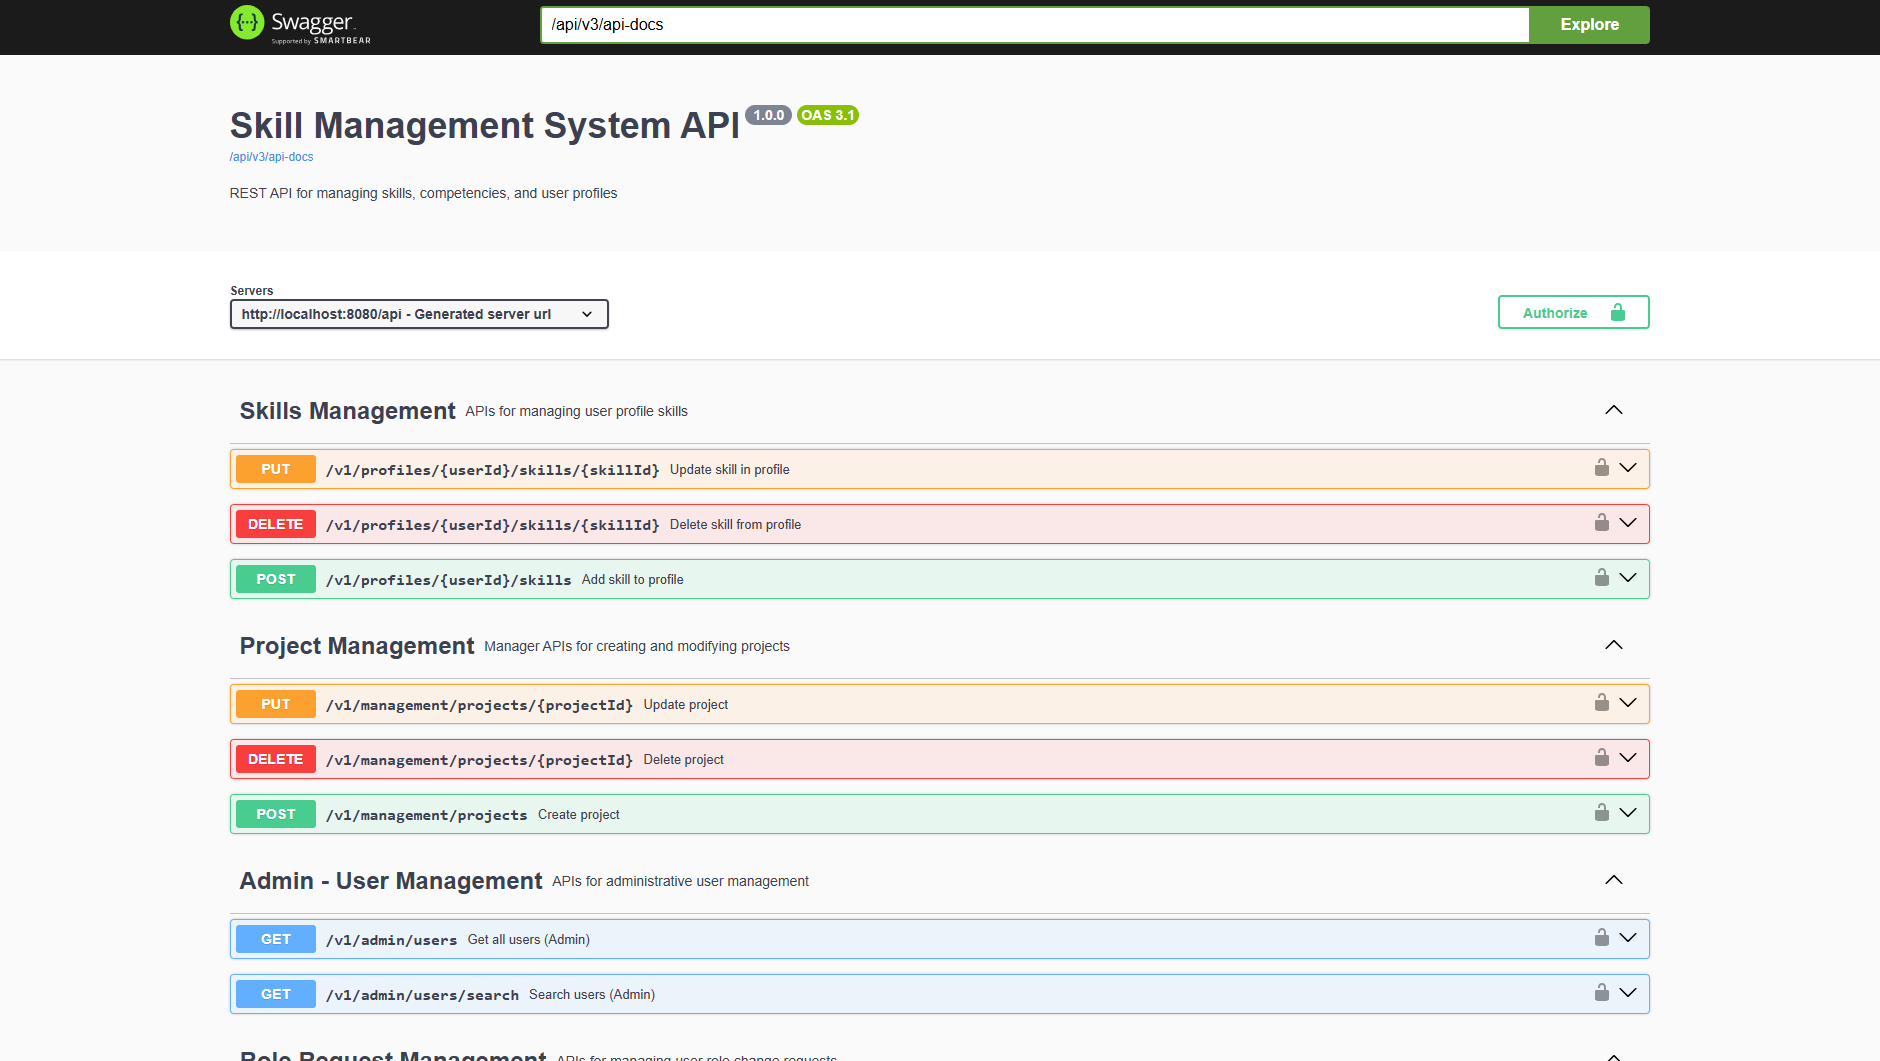
\includegraphics[width=\textwidth]{references/schnittstellen-doku-1.png}
\caption{API-Dokumentation: Übersicht der verfügbaren Endpunkte gruppiert nach Funktionsbereichen}
\label{fig:api_documentation}
\end{figure}

\subsubsection{Vollständige API-Endpunkt-Übersicht}

Die folgende Tabelle listet alle implementierten API-Endpunkte mit HTTP-Methode, Pfad, Beschreibung und erforderlicher Rolle auf:

\begin{table}[H]
\centering
\tiny
\rowcolors{2}{EDAGDunkelgrau!10}{white}
\begin{tabularx}{\textwidth}{|l|l|X|l|}
\hline
\rowcolor{EDAGDunkelgrau!30}
\textbf{Methode} & \textbf{Endpunkt} & \textbf{Beschreibung} & \textbf{Rolle} \\
\hline
\multicolumn{4}{|l|}{\cellcolor{EDAGDunkelgrau!10}\textbf{Skills Management}} \\
\hline
PUT & /v1/profiles/\{userId\}/skills/\{skillId\} & Update skill in profile & USER \\
\hline
DELETE & /v1/profiles/\{userId\}/skills/\{skillId\} & Delete skill from profile & USER \\
\hline
POST & /v1/profiles/\{userId\}/skills & Add skill to profile & USER \\
\hline

\multicolumn{4}{|l|}{\cellcolor{EDAGDunkelgrau!10}\textbf{Project Management}} \\
\hline
PUT & /v1/management/projects/\{projectId\} & Update project & MANAGER \\
\hline
DELETE & /v1/management/projects/\{projectId\} & Delete project & MANAGER \\
\hline
POST & /v1/management/projects & Create project & MANAGER \\
\hline

\multicolumn{4}{|l|}{\cellcolor{EDAGDunkelgrau!10}\textbf{Admin - User Management}} \\
\hline
GET & /v1/admin/users & Get all users (Admin) & ADMIN \\
\hline
GET & /v1/admin/users/search & Search users (Admin) & ADMIN \\
\hline

\multicolumn{4}{|l|}{\cellcolor{EDAGDunkelgrau!10}\textbf{Role Request Management}} \\
\hline
GET & /v1/role-requests & Get role requests by status & USER \\
\hline
POST & /v1/role-requests & Create role request & USER \\
\hline
POST & /v1/role-requests/\{requestId\}/reject & Reject role request & ADMIN \\
\hline
POST & /v1/role-requests/\{requestId\}/approve & Approve role request & ADMIN \\
\hline
GET & /v1/role-requests/me & Get my role requests & USER \\
\hline
DELETE & /v1/role-requests/\{requestId\} & Cancel role request & USER \\
\hline

\multicolumn{4}{|l|}{\cellcolor{EDAGDunkelgrau!10}\textbf{Profile Management}} \\
\hline
GET & /v1/profiles/\{userId\} & Get user profile & USER \\
\hline
PUT & /v1/profiles/\{userId\} & Update user profile & USER \\
\hline

\multicolumn{4}{|l|}{\cellcolor{EDAGDunkelgrau!10}\textbf{Employee Discovery}} \\
\hline
GET & /v1/employees/\{userId\} & Get employee by ID & USER \\
\hline
GET & /v1/employees/search & Search employees & USER \\
\hline
GET & /v1/employees/filter-options & Get filter options & USER \\
\hline

\multicolumn{4}{|l|}{\cellcolor{EDAGDunkelgrau!10}\textbf{Projects}} \\
\hline
GET & /v1/projects/\{projectId\} & Get project by ID & USER \\
\hline
GET & /v1/projects/users/\{userId\} & Get user projects & USER \\
\hline
GET & /v1/projects/search & Search manager's projects & MANAGER \\
\hline
GET & /v1/projects/filter-options & Get project filter options & USER \\
\hline

\multicolumn{4}{|l|}{\cellcolor{EDAGDunkelgrau!10}\textbf{Analytics \& Activities}} \\
\hline
GET & /v1/analytics/users/\{userId\}/statistics & Get user statistics & USER \\
\hline
GET & /v1/analytics/users/\{userId\}/skill-trends & Get skill development trends & USER \\
\hline
GET & /v1/analytics/users/\{userId\}/activities & Get recent activities & USER \\
\hline

\multicolumn{4}{|l|}{\cellcolor{EDAGDunkelgrau!10}\textbf{Reference Data Options}} \\
\hline
GET & /v1/options/skills & Get all available skills & USER \\
\hline
POST & /v1/options/skills & Create skill (Admin) & ADMIN \\
\hline
GET & /v1/options/skill-categories & Get skill categories & USER \\
\hline
POST & /v1/options/skill-categories & Create skill category (Admin) & ADMIN \\
\hline
GET & /v1/options/positions & Get available positions & USER \\
\hline
POST & /v1/options/positions & Create position (Admin) & ADMIN \\
\hline
GET & /v1/options/locations & Get available locations & USER \\
\hline
POST & /v1/options/locations & Create location (Admin) & ADMIN \\
\hline
GET & /v1/options/skills/category/\{categoryId\} & Get available skills by category & USER \\
\hline
\end{tabularx}
\caption{Vollständige REST-API-Endpunkt-Übersicht des Skill Management Systems}
\label{tab:api_endpoints}
\end{table}

\textbf{Authentifizierung:} Alle Endpunkte erfordern einen gültigen JWT Access Token im Authorization-Header (\texttt{Bearer <token>}). Die Token-Validierung erfolgt via Keycloak Token Introspection (siehe Sequenzdiagramm in Abbildung~\ref{fig:auth_sequence}).
